%
% Optical Design Chapter
%
% Author:
% Version:
%
%
% Optical Design Chapter
%
% Author:
% Version:
%

\FloatBarrier
\subsection{Executive Summary}
%\emph{Responsible:   WP3 coordinator, A. Freise   \\}

The optical design of the Einstein Telescope refers to the design of
the laser interferometer, the core instrument in which the
effect of a passing gravitational wave is
transformed into a read-out signal, measuring the changes 
in the distance between suspended mirrors using ultra-stable
laser beams. The amplitude of this signal
scales at first linearly with the light power stored in the  
interferometer arms. This led to the development of long-baseline
detectors utilising high-power lasers. The interferometers of 
first generation GW detectors were already extremely sensitive 
to arm length changes (and thus to gravitational waves). Their sensitivity
over a wide frequency range was limited not by technical inaccuracies 
but by intrinsic noise of their fundamental parts, such as the quantum
fluctuation of the laser light. The optical design efforts since then
have focused on developing and implementing advanced
optical technologies to reduce the impact of these noise sources 
on the read-out signal.

Gravitational waves exist in two distinct polarisations. To capture the
full signal a GW observatory should be able to detect both polarisations at
all times. This can be achieved by employing multiple co-located
detectors. The optimal footprint of the observatory will depend on the
geographical details of the yet unknown location. It is possible to
position three detectors in a triangle as shown in Figure~\ref{fig:ET_full_triangle}.
Such a triangular shape represents the minimal topological solution and
has been chosen as the baseline geometry for ET.
\begin{figure}[h]
	\centering
		\includegraphics[width=0.6\textwidth]{Sec_Optics/ET_full_april2011.pdf}
	\caption{Schematic full view of the optical layout of the ET
    Observatory. 
 the full instrument consists of 3 pairs of km-scale
    interferometers positioned such that they form a triangular
    shape. Each interferometer pair represents one wide-band detector,
    in which one interferometer is optimised for gravitational waves
    at low frequencies (LF) and the other for high frequencies (HF).
Please note that this graphic is not too scale and does not show the exact position of the
optical components. Instead, it provides an overview of the general shape and
complexity of the optical layout of the main interferometers.
}
	\label{fig:ET_full_triangle}
\end{figure}

The core interferometers of the Einstein Telescope will be advanced
Michelson interferometers
with an arm length of 10\,km, a length which was a given input
parameters for the optical design. Some technologies for noise
reduction are not necessarily compatible with each other. Therefore
the optical design includes two parallel, 10\,km long interferometers per detector,
one interferometer being optimised for low-frequency (LF) gravitational
waves, the other covering the high frequency (HF) part of the spectrum; 
this approach has been called `xylophone' design.
The main characteristics of the two interferometer types are:
\begin{itemize}
\item the \textbf{HF} interferometer is a room temperature
  interferometer with very high laser power and fused silica test
  masses similar to Advanced
  detectors, but using an alternative laser beam shape,
the Laguerre-Gauss LG33 mode.
\item the \textbf{LF} interferometer is a cryogenic
  interferometer with medium laser power, using silicon test
  masses and a laser system with a 1550\,nm wavelength.
\end{itemize}

One of the main noise sources to suppress by means of optical
design is the quantum noise of the light.
A detailed study of newly proposed schemes for quantum
noise reduction, such as speed meters or optical bars has been
undertaken and two interesting candidates have been identified:
the ET baseline design will make use of dual-recycled Michelson
interferometers, very similar to those planned for Advanced LIGO, with
the additional injection of frequency-dependent squeezed light 
into the dark port. In parallel, we will continue to study speed-meter
like configurations, in particular those based on the Sagnac topology.

The choice of using Michelson interferometers (with recycling techniques) has the
great advantage that much of the research and development towards
the Advanced detectors can be applied directly. In particular, for the
conceptual designs of auxiliary systems such as input-output optics, 
the interferometer control or the thermal control of the
interferometer mirrors, we can adapt the current state of the art
with only small envisaged changes.

\vspace{5mm}
A summary of all the optical parameters of the Einstein Telescope
baseline design is given in the table below:
\begin{longtable}{p{5.5cm} *{2}{p{5cm}}}
	%%% HEADER, repeats on every page
	&	 \textbf{ET-HF}   	&	 \textbf{ET-LF} 	\\
\noalign{\smallskip}\hline\hline\noalign{\smallskip}
\endhead

%%% generic parameters for the whole itf
Approximate frequency range	&	10--$10^4$\,Hz 	&	1--250\,Hz	\\
Detection scheme	&	DC readout	& DC readout	\\
Input power (after IMC) 	&	500\,W 	&	3\,W 	\\
Laser wavelength 	&	1064\,nm 	&	1550\,nm 	\\
Beam shape 	&	LG$_{33}$	&	TEM$_{00}$	\\

%%% ARM CAVITIES
\noalign{\smallskip}\hline\noalign{\smallskip}					
\multicolumn{3}{c}{\textit{ARM CAVITIES}}	\\				
\noalign{\smallskip}\hline\noalign{\smallskip}					

Arm length 	&	10\,km	&	10\,km 	\\
Opening angle	&	$60\,^\circ$	&	$60\,^\circ$	\\
Arm power 	&	3\,MW 	&	18\,kW	\\
Temperature 	&	290\,K 	&	10\,K  	\\
Mirror material 	&	fused silica 	&	silicon  	\\
Mirror diameter	&	62\,cm	&	>45\,cm	\\
Mirror thickness 	&	30\,cm	&	about 50\,cm	\\
Mirror mass	&	200\,kg 	&	211\,kg 	\\
Beam radius (at mirror)	&	7.2\,cm 	&	9.0\,cm	\\
Beam waist (symmetric cavity)	&	2.51\,cm	&	2.9\,cm	\\
RoC (symmetric cavity)	&	5690\,m	&	5580\,m	\\
%Rayleigh range (symmetric cavity)	&	1860\,m	&	1700\,m	\\
Scatter loss per surface 	&	37.5\,ppm 	&	37.5\,ppm 	\\
Finesse	&	880		&	880		\\
Reflective coating ITM	&	tantala/silica	&	tantala/silica	\\
	& 	8 $\lambda/4$ doublets	&	9 $\lambda/4$ doublets	\\
Reflective coating ETM	&	tantala/silica	&	tantala/silica	\\
	&	17 $\lambda/4$ doublets	&	18 $\lambda/4$ doublets	\\
Transmission ITM	&	7000\,ppm	&	7000\,ppm	\\
Transmission ETM	&	6\,ppm	&	6\,ppm	\\

%%% CENTRAL INTERFEROMETER
\noalign{\smallskip}\hline\noalign{\smallskip}					
\multicolumn{3}{c}{\textit{CENTRAL INTERFEROMETER}}	\\				
\noalign{\smallskip}\hline\noalign{\smallskip}					

SR-phase 	&	tuned (0.0) 	&	detuned (0.6)	\\
Focussing element	&	in or near the ITM 	&	in or near the ITM	\\
                	& 	focal length $= 303$\,m	&	focal length $= 303$\,m	\\
Distance ITM--BS	&	300\,m	&	300\,m	\\
Distance BS--MPR	&	10\,m	&	10\,m	\\
Recycling cavity length	&	310\,m	&	310\,m	\\
Beam size on BS	&	4.7\,mm	&	6\,mm	\\
Beam size on MPR	&	2.7\,mm	&	3.4\,mm	\\
Recycling gain	&	21.6	&	21.6	\\
Recycling cavity free spectral range	&	484\,kHz	&	484\,kHz	\\
%Rayleigh range in central IFO	&	40\,m	&	47.0\,m	\\
Round-trip Guoy phase	&	$10.5\,^\circ$	&	$9.6\,^\circ$	\\
mode separation frequency	&	28\,kHz	&	26\,kHz	\\
Recycling cavity temperature	&	room temperature	&	room temperature	\\
Beam splitter material	&	fused silica	&	fused silica	\\
%Beam splitter diameter	&	?	&	around 50\,cm	\\
%Beam splitter thickness	&	?	&	about 30\,cm	\\
%Beam splitter coating	&	?	&	tantala/silica	\\
%	&	&	3 $\lambda/4$ doublets (upper limit)	\\
Transmission PRM	&	4.6\,\%	&	4.6\,\%	\\
Transmission SRM	&	10\,\% 	&	20\,\% 	\\

%%% FILTER CAVITIES
\noalign{\smallskip}\hline\noalign{\smallskip}					
\multicolumn{3}{c}{\textit{FILTER CAVITIES}}	\\				
\noalign{\smallskip}\hline\noalign{\smallskip}					
Quantum noise suppression 	&	frequency-dependent squeezing	&	frequency-dependent squeezing	\\
Filter cavities 	&	$1 \times 300\,$m  	&	$2 \times 10\,$km	\\
%Squeezing level  	&	refer to~\ref{fig:sqzHF} 	&	refer to Fig.~\ref{fig:sqz} 	\\
Half-bandwidth	&	5.7\,Hz	&	5.7\,Hz and 1.5\,Hz\\
%Resonance frequency	&	?	&	$2\pi\cdot 6.6\,Hz$ / $-2\pi\cdot 25.4\,Hz$	\\
Detuning	&	25.4\,Hz	&	25.4\,Hz and 6.6\,Hz\\
Round-trip loss	&	75\,ppm	&	75\,ppm	\\
%Coupling mirror reflectance	&	?	&	98.8864\% / 99.5323\%	\\
\noalign{\smallskip}\hline\noalign{\smallskip}					

%%% SUSPENSIONS
%\multicolumn{3}{c}{\textit{SUSPENSIONS}}	\\				
%\noalign{\smallskip}\hline\noalign{\smallskip}				
%Seismic isolation 	&	SA, 8\,m tall 	&	mod SA, 17\,m tall 	\\
%Seismic (for $f>1$\,Hz) 	&	$5\cdot 10^{-10}\,{\rm m}/f^2$ 	&	$5\cdot 10^{-10}\,{\rm m}/f^2$  	\\
%Gravity gradient subtraction 	&	none 	&	none 	\\
%\noalign{\smallskip}\hline\noalign{\smallskip}					
%\multicolumn{3}{c}{\textit{INJECTION OPTICS}}	\\				
%\noalign{\smallskip}\hline\noalign{\smallskip}					
%Intensity noise	&	TBD	&	TBD	\\
%Beam jitter noise	&	TBD	&	TBD	\\
%Overall throughput	&	$>50\%$	&	$>50\%$	\\
%IMC cavities	&	$2\times 20$\,m	&	$2\times 20$\,m	\\
%	&	even number of mirrors	&	triangular cavities	\\
%IMC cavities throughput	&	$>80\%$	&	$>80\%$	\\
%IMC mirrors substrate	&	fused silica 	&	?	\\
%IMC coating absorption	&	$<1$\,ppm	&	?	\\
%\noalign{\smallskip}\hline\noalign{\smallskip}					

%%% DETECTION OPTICS
% \multicolumn{3}{c}{\textit{DETECTION OPTICS}}	\\				
% \noalign{\smallskip}\hline\noalign{\smallskip}					
% Detection scheme	&	?	&	?	\\
% \noalign{\smallskip}\hline\noalign{\smallskip}					

\end{longtable}



%%% TODO: add more here, at least covering filter cavities and LG
%%% modes. Could also quickly run through the list of optical 
%%% parameters?





\FloatBarrier
\subsection{Description}
%\emph{Responsible:  WP3 coordinator, A. Freise  \\}

Modern gravitational wave detectors are based on km-scale laser interferometers.
Also the Einstein Telescope is using a sophisticated laser
interferometer
to convert the signal of a passing gravitational wave into a readout
signal that can be processed electronically. The basic
interferometer design is still similar to that of the original
interferometer by Michelson (used more than 100 years ago in the famous Michelson and Morley
experiment to disprove the existence of a so-called aether). However,
to achieve better sensitivities 
the interferometry has been refined and extended continuously, especially during
the last two decades, driven by the gravitational wave community. As a result, modern
interferometers are now able to reach unprecedented sensitives beyond the Standard
Quantum Limit of interferometry. At the same time the optical design
has become a more challenging task. Modern interferometers couple all
involved optical systems into one closely coupled, complex machine. 

The focus of the optical design was to identify and develop an optical layout for the
core interferometer of a third generation detector which includes
advanced optical technologies required to reach the target sensitivity
of the ET detector. The term `optical layout'  includes a number of
layers of complexity in optical design: first of all, the core
interferometer is the part of the detector which converts the
gravitational wave signal into a measurable optical signal. Second,
the core interferometer by design couples all auxiliary subsystems
together. Thus part of the effort in this design study was dedicated to how the
signal and all possible noises couple into the detector output.  And
third the optical layout largely defines the type of instrument,
i.e.\ it defines the shape of the detector, the type of interferometry
used, as well as which advanced optical technologies are included.

In order to achieve the envisaged sensitivity of the Einstein
Telescope, once again the interferometry must be pushed beyond
the state-of the art. For the first time a number of advanced
technologies such as cryogenic mirrors, squeezed light and 
alternative beam shapes are to be combined in one system.
This section describes in detail the design process towards the
optical layout of ET which forms the baseline for the design of the
infrastructure, as well as the mirror suspension systems.
%% --- adf
All the currently active GW detectors are L-shaped, with orthogonal
arms; although this geometry maximises the sensitivity of the single
detector with respect to the arm length, other geometries are
possible. In particular, triangular-shaped detectors have been
proposed in the past; the LISA geometry is also triangular.
 Two L-shaped
detectors, forming a 45 degrees angle, could fully resolve the two
polarisation amplitudes of the incoming wave. Obviously in an
underground site, the realization of this geometry is
difficult, due to the high cost of the infrastructure. If the angle
between the two arms of each
detector is reduced to 60 degrees, three detectors can be accommodated
in a triangular-shaped underground site, minimizing the required
number
of caverns. An
analysis of a triangular-shaped
third generation GW observatory is described in
sections~\ref{sec:georeview}
%and \ref{sec:toporeview} 
with the conclusion that if a site that can
accommodate a triangular observatory is found, 
the triple co-located interferometers will be the best choice and the
triangular shape has been adopted as the baseline for the current
ET design.

Each detector within a triangular observatory can in principle be composed of
one or several interferometers of different topology. It can be shown
that one interferometer per detector is not ideal.
Spanning the wide detection band envisaged for ET is technically
extremely challenging: Different noise types dominate the various
frequency bands and often these noises show opposite response for
changing the involved design parameters. Sometimes the reduction
techniques for different noise types are incompatible. 
A well-known example for a parameter that affects different frequency
regions differently is the correlation of the two quantum noise
components: photon shot noise and photon radiation pressure
noise. In order to improve the shotnoise-limited sensitivity at high
frequencies one needs to increase circulating optical power,
which at the same time increases the radiation pressure noise and therefore worsens
the low frequency sensitivity. Alternatively, lowering the circulating
power reduces the radiation pressure effects and improves the low frequency sensitivity,
while the shotnoise contribution will rise and reduce the high frequency
sensitivity. 
This dilemma can be resolved by following the path of electromagnetic
astronomy, where telescopes are being built for a specific, rather
narrow-banded detection window (visible, infrared etc) and later on
the data from different frequency bands are combined to cover the
desired bandwidth.  Building two interferometers, each optimised
for reducing the noise sources at one specific frequency band, can
form a xylophone observatory providing substantially improved
broadband sensitivity. 
We have developed a
2-band xylophone detector configuration to resolve the high-power
low-temperature problem of a single band ET observatory as described
in section~\ref{sec:optlayout}.  Based on this design envelope of
three xylophone detectors in a triangular setup, a more detailed
design of the optical layout can be performed. 
This formed the basis for the investigation into the required cavern
size and associated infrastructure impact,
see section~\ref{sec:SiteInfra}.

%%% Topology Choice, Quantum noise reduction, Squeezed light
Currently the Michelson interferometer topology is used in
laser-interferometric gravitational wave detectors. However,
alternative topologies, such as the Sagnac interferometer or so-called
`optical bars',  have been suggested and would also fit into a triangular, xylophone based detector. The main
attraction of alternative interferometer topologies is that
they allow the implementation of different quantum noise reduction
schemes. While classical interferometers are limited by the Standard
Quantum Limit, a noise floor composed of photon shotnoise and
radiation pressure effects, clever interferometer designs and the use
of squeezed light allow us to push beyond that limit. A detailed study 
of a wide range of possible quantum noise reduction schemes has
been undertaken and is reported in sections~\ref{sec:qnr} and
\ref{app:QNR}.
As the outcome of this study, taking into account technical considerations, a 
Michelson-based topology with Signal Recycling and squeezed light
injection has been selected for the Einstein Telescope baseline.
The study also showed that Sagnac-based speedmeter topologies are an appealing 
alternative and should be studied further.
The chosen design implements so-called filter cavities to generate the
frequency-dependent squeezed light. During the course of the design
study a lot of original research has been undertaken to derive
requirements for such cavities and their implementation, details
are reported in appendix~\ref{app:filtercavities}.

%%% Details
With the baseline of the optical layout selected, the design progressed
into essential subsystems. The core element of these laser
interferometers are the large principal mirrors of the arm
cavities. The
thermal noise of these mirrors represents one of the main limits to
the achievable sensitivity. Towards the realisation of
second-generation interferometric detectors, a major research effort
is underway to study and improve all aspects of these mirrors,
especially the quality of the dielectric coatings. This work has been
extended here to determine the requirements for the Einstein
Telescope. A further challenge is to identify the best material and
design choices for the cryogenic mirrors to be used in the
low-frequency interferometer. Two solution based on Sapphire and
silicon as mirror bulk material have been
identified and carefully studied in section~\ref{sec:optcomps} alongside
fused-silica mirrors for the high temperature interferometer. This
work is complemented by tables stating the optical, mechanical and thermal 
properties in appendix~\ref{sec:app}.

The following sections~\ref{sec:injection}, \ref{sec:detection}, \ref{sec:control}
and \ref{sec:tcs} provide details about auxiliary optics system, such as the
injection
optics, providing the laser beam to the main interferometer, the
detection system, responsible for converting optical into electrical
signals and the control systems required to maintain a stable
operating position of the entire interferometer. The design of these
systems is a direct application and extension of the work done 
and experience gained with the first and second generation of 
detectors and we expect future changes to these systems based
on the experience gained when the advanced detectors
start operating. 

Building on the detailed baseline design of the optical layout as well as
the main subsystems, section~\ref{sec:opti_costs}  provides a cost
evaluation of the optical
system for the Einstein Telescope. We also provide 
a guide to future R\&D activities by outlining in section~\ref{sec:RD} 
which of the technologies require
major R\&D efforts before they could be incorporated in a technical  
design of the Einstein Telescope.

%%% Alternative technologies

During the course of the design study we have also investigated a
number of new and hypothetical effects or technologies. One 
hypothesis that gained popularity for a while proposes a new kind of
noise originating 
from the holographic principle of unification physics, which can arise in the 
high-precision interferometry \cite{2009_holonoise}. We investigated
this so-called holographic 
noise (cf. Appendix~\ref{app:holo}) and came to the conclusion that it
is so far insufficiently developed and verified from both theoretical
and experimental sides, and we do not expect it to have any impact of
the design of ET. 
Further, a technique proposed to eliminate all types of
noise associated with the motion of test masses is the so-called
\emph{displacement-noise free interferometry}. Also this has been
investigated in Appendix~\ref{app:DFI}, but dismissed as it currently provides no route towards
a realistic experimental implementation. 

\FloatBarrier
\subsection{Review on the geometry of the observatory}\label{sec:georeview}
%\emph{Author(s): \textbf{Andreas Freise}, Stefan Hild} \\

This section briefly reviews the reasoning behind the shape of current gravitational wave detectors and then
discusses alternative geometries which can be of interest for third-generation detectors. We
will use the terminology introduced in the review of a triangular configuration~\cite{Freise2009} and
discriminate between the
\emph{geometry}, \emph{topology} and \emph{configuration} of a detector as follows:
\begin{itemize}
\item The \emph{geometry} describes the position information of one or several interferometers,
defined by the number of interferometers, their location and relative orientation.
\item The \emph{topology} describes the optical system formed by its core elements.
The most common examples are the Michelson, Sagnac and Mach--Zehnder topologies.
\item The \emph{configuration} describes the detail of the optical layout and the set of parameters that
can be changed for a given topology, ranging from the specifications of the optical core
elements to the control systems, including the operation point of the
main interferometer. Also the
addition of optical components to a given topology is often referred to as a change in configuration.
\end{itemize}

\FloatBarrier
\subsubsection{The L-shape}
\label{sec:lshape}
Current gravitational wave detectors represent the most precise instruments for measuring length changes.
They are laser interferometers with km-long arms and are operated differently from many precision
instruments built for measuring an absolute length. Viewed from above
they resemble an L-shape with equal arm length.
This geometric form follows directly from the nature of gravitational
waves: gravitational waves are transverse, quadrupole waves, thus a length change measured along any axis
occurs with opposite sign along the axis orthogonal to the previous one and the direction of propagation.
This key feature allows us to make a differential measurement between two orthogonal interferometer
arms, yielding twice the amplitude of a single arm. More importantly, a differential measurement allows us to
potentially discriminate between gravitational wave signals and those types of noise common to both arms, such as,
for example, laser amplitude noise. To achieve this the interferometer arms generally have to have approximately
the same length. The most simple L-shaped interferometer capable of doing this type
of measurement is the symmetric Michelson interferometer, on whose topology all current interferometric detectors
are based.

The long arm length of the detectors represents the simplest way to increase the signal-to-noise ratio
in the detector because for wavelength larger than the detector
dimensions, the `tidal' effect of the gravitational wave increases with the base length over which the
measurement is taken. In contrast the fundamental noises are connected to the interaction
of light with the optical components or the photo detection and thus do not scale with the length of the interferometer
arms.
We can summarise that for typical ground-based detectors with
sufficiently good vacuum and mirror position control systems, an increase in arm length will increase the
sensitivity of the detector proportionally.


Using the framework developed in~\cite{Jaranowski:1998qm} we can compute the sensitivity of a laser interferometer
with two arms to gravitational waves, taking into account the geometry of the detector, the location of the source and the
changes of both over time. The equations show directly that the arms of the detector do not
have to be perpendicular. A right angle, however, provides the maximum
response of an ideal detector to gravitational waves, which more generally can be written as
\begin{equation}
h(t)=F_{+}(t)h_{+}(t)+F_{\times}(t)h_{\times}(t)=\sin\zeta\,f(t,\psi, \dots)
\end{equation}
with $\zeta$ the opening angle of the interferometer arms, $F_{+}$ and $F_{\times}$ the beam pattern functions
and $f(t,\psi, \dots)$ a function of the remaining parameters describing the geometry (the location of the detector and
of the source in space and time and the wave polarisation angle).

In summary we can say that for a gravitational wave of given direction and polarisation, a properly aligned  symmetric L-shape
is an ideal optical layout for an interferometric
detector; the arms should be as long as possible and the sensitivity is maximised for an opening angle of $90^\circ$.
It should be noted that this does not put severe constraints on the type of interferometer topology used. In fact,
most common interferometer types can be used in a form that features two large symmetric arms in an L-shape
while potential other interferometer arms or sections are shortened such that they can be considered as part of one
corner of the detector.

\FloatBarrier
\begin{figure}[tbh]
\begin{center}
\includegraphics[width=0.7\textwidth,keepaspectratio]{Sec_Optics/TRIMI03}
\caption{{\bf a)} Triangle geometry: three L-shaped detectors with 10\, km arm length
are positioned in a equilateral triangle.
{\bf b)} Four L-shaped detectors at $0^\circ$ and $45^\circ$. The integrated length of all
interferometer arms in both configurations is 60\,km and two interferometer arms can share
the same structure. Note that for avoiding noise correlations between two detectors the
neighbouring interferometer arms would probably be housed in a separate vacuum tubes.}
\label{fig:triangle}
\end{center}
\end{figure}
\subsubsection{The triangle}
At any given moment an L-shaped detector can only detect one linear combination of polarisations of a
gravitational wave. However, for
estimation of source parameters from the measured signal, the full polarisation information is essential.
Thus it is of considerable interest to design a detector that is able to detect both polarisations (and thus the full content)
of a gravitational wave at all times. This can be achieved by combining two co-located
L-shaped detectors which are positioned at $45^\circ$ to each other. % (as shown in Figure~\ref{fig:triangle}).
More than 20 years ago it was recognised that a triangular geometry would provide the same
sensitivity to both polarisations as detectors at $45^\circ$ whilst requiring less enclosed space and fewer
end stations~\cite{Winkler1985}. In particular, the sensitivity of the two geometries shown
in Figure~\ref{fig:triangle} differs only by $6\%$~\cite{Freise2009}. The difference in the sensitivity to
different polarisations between a single L-shape and a triangular geometry can be best illustrated
with a plot of the so-called antenna pattern as shown in Figure~\ref{fig:triangleAP}.


\begin{figure}[t]
\begin{center}
\includegraphics[width=0.9\textwidth, viewport= 50 0 885 370]{Sec_Optics/ap_mi_trimi.pdf}
\caption{The response of a detector to a linear polarised gravitational wave
as a function of the detector orientation. Both plots show the normalised sensitivity
to a wave travelling along the z-axis. Each data point represents the sensitivity of the
detector for a specific detector orientation defined by the detector normal
passing the respective data point and the origin. The colour
of the data point as well as its distance from the origin indicate the magnitude of the
sensitivity. The left plot depicts the response of a single Michelson, while the right plot
gives the response of a set of three interferometers in a  triangular geometry.
}
\label{fig:triangleAP}
\end{center}
\end{figure}
Using co-located detectors yields another advantage. Both layouts shown in Figure~\ref{fig:triangle} represent
detectors with redundancy. Redundancy here can be understood in relation to the continuous operation of the
detector as an observatory, or as a feature of the data streams generated by the full system. Redundancy in operation
is achieved by having multiple detectors which generate an equal or similar response to gravitational waves.
This is desirable in observatories which are expected to produce a quasi-continuous stream of astrophysically meaningful
data over a substantial amount of time. Typically laser interferometers cannot produce science data during
upgrades and maintenance work. Thus only alternating upgrades and data taking of redundant detectors can
avoid long down-times, for example during detector upgrades.

Such redundancy is obviously provided in the case of the 4 L-shaped  detectors, where two detectors are
always identical but can be operated independently. However, one can easily show that the triangular geometry
provides exactly the same redundancy~\cite{Freise2009}. For example, for three equal L-shaped interferometers
oriented at $0^\circ$, $120^\circ$ and $240^\circ$, one obtains:
\begin{equation}
-h_{0^\circ}= h_{240^\circ}+h_{120^\circ}\,,
\end{equation}
where the sign of the operation is defined by which ports of the interferometers
are used to inject the laser light. Thus the two interferometers at $120^\circ$ and $240^\circ$
create exactly the same response as the one at $0^\circ$. This allows
us to construct
so-called null-streams (or null-data streams)~\cite{GurselTinto1989}. Null-streams are a powerful
data analysis method that allows one to identify noise that is uncorrelated between the
detectors. Even though this does not increase the strain sensitivity of a detector,
it can add significantly to the robustness of the data processing
pipelines and thus to a larger number of detected events.
%lead, for example, to shorter delays between an event and the generation of a trigger for follow-up searches with optical telescopes.
The triangular geometry represents the minimal setup in one plane that can resolve both polarisations
and provides redundancy for the generation of null-streams.

\FloatBarrier
%\subsubsection{Interferometer Topologies }\label{sec:topologies}
To date no laser interferometer topology other than the Michelson has been
used for gravitational wave detection. However, some very advanced
noise reduction techniques proposed for future
detectors are based on topologies of the Sagnac interferometer, the Fox-Smith cavity or the
Mach-Zehnder interferometer~\cite{Chen2003,danilishin2006,Chen06b}.

It is worth noting that a triangular geometry as discussed above
is compatible with different interferometer
topologies. In particular it is possible to use different
topologies while maintaining the {\sf L}-shape of the single
interferometers
as displayed in figure~\ref{Fig:Lshape}.
Therefore, for example, three Sagnac interferometers or three cavities
could be used to form a triangle.
Such detector designs can provide similar benefits as described above for the
triple Michelson geometry so that the triangular geometry is largely independent
of the topology of the individual interferometers.

\longetbox{i}{ibox:topopt}{Different topology options}
{In this box we will list the different main interferometer
topologies that can be used for gravitational-wave detection and
describe their basic optical systems. A full gravitational-wave
detector could actually consist of more than one of those main
interferometers and could also be equipped with additional
techniques in order to achieve a specific susceptibility to the
quantum noise as will be described in Sec.~\ref{sec:qnr}.
Note that in principle, all of the mentioned interferometer
topologies can be fitted into
\begin{figure}[H]
\centering
\includegraphics[width=15cm]{./Sec_Optics/Lshape.pdf}
\caption{Different (basic) topology options: simple Michelson
interferometer topology (left panel); zero-area Sagnac
interferometer topology (midd3le panel); optical bar topology
(right panel)
}\label{Fig:Lshape}
\end{figure}
an L-shape or into another two-arm shape under an arbitrary angle,
as shown in Fig.~\ref{Fig:Lshape}.
\begin{itemize}
\item {\bf Michelson interferometer} (basic): a laser beam is
split at a beam splitter and sent along two perpendicular
interferometer arms (cf.\ left panel of Fig.~\ref{Fig:Lshape}). The
ends of these arms (north and east) are marked by highly
reflective identical end mirrors, which reflect the beams back
into themselves so that they can be recombined at the beam
splitter. Generally, the Michelson interferometer has two outputs,
the south port and the west port (which is also the input port).
Both output ports can be used to obtain interferometer signals,
however, most setups are designed in such a way that the signals
are detected at the south port. For the detection of gravitational
waves, the Michelson interferometer has to be sensitive to small
perturbations in the difference of the two arm lengths and the
phase relation is chosen in such a way that this signal interferes
constructively at the south port.
Usually the south port is kept
nearly dark, with all light reflected back to the west input port,
then also called the bright port of the interferometer. A
power-recycling mirror can be positioned at the bright port in
such a way that it forms a resonant cavity for the carrier light
together with the mirrors of the two interferometer arms.
Furthermore, each interferometer arm can be replaced by equal
Fabry-Perot cavities, formed by an input mirror and an
end mirror. An additional mirror can also be placed at the
interferometer's south port, known as the signal-recycling mirror.
Another possibility is to send the output signal at the west port
into an additional resonator, a so-called sloshing cavity.
Furthermore, polarizing optics can be used in order to send the
beam back into the interferometer. The Michelson interferometer is
the standard topology for interferometric gravitational-wave
detectors. The great advantage of this configuration is that there is a lot of
experience gathered.
\item  {\bf Sagnac interferometer} (basic): a laser beam is split
into two beams at the beam splitter which both travel through the
whole interferometer but in opposite directions. The two beams are
recombined at the beam splitter. The interferometer has only one
output port, namely the south port. A Sagnac
interferometer is by construction always operated at a dark port, i.e.
all carrier light is reflected back to the input port. The
arms can be folded in such a way that both beams circulate around
a zero area (cf.\ middle panel of Fig.~\ref{Fig:Lshape}) in order
to make the interferometer insensitive to rotations and forming
two perpendicular interferometer arms. Those arms can be replaced
by ring resonators, either of rectangular or triangular shape. For
the Sagnac interferometer topology, an additional mirror at the
input port can realize power-recycling and an additional mirror
at the output port can realize signal-recycling. Up to now a
Sagnac interferometer has never been adopted as a large-scale
interferometric gravitational-wave detector. Only some features
have been tested in table-top experiments and a theoretical study
has started to explore noise couplings in a Sagnac
interferometer~\cite{Chelkowski}.
\item {\bf Optical bar}: The optical bar topology is an optical
realization of a mechanical resonant bar gravitational-wave
detector. It essentially consists of two coupled optical
resonators, which are shaped as a L and coupled through a light,
partially transmissive mirror as shown in the right panel of
Fig.~\ref{Fig:Lshape}. An additional local meter is applied to the
central mirror, reading out its motion. The local meter could in
principle be any device but its sensitivity is essentially
determining the sensitivity of the optical bar detector. It is
even not obligatory for the local meter to be an optical device,
for instance it could be a SQUID-based microwave meter as a speed
meter, or some other high precision superconductive sensor. The
optical bar topology can be transformed into an optical lever
topology by inserting an additional mirror into each arm of the L,
forming a resonant cavity together with the corresponding end
mirror.
\end{itemize}}

The case for alternative topologies is largely based on ideas for the
reduction of quantum noise. In general, the signal-to-noise ratio of a
single interferometer is different for each topology, with the actual
difference depending also on the type of noise under investigation.
However, it is not possible to identify a topology with a meaningful
signal-to-noise ratio or sensitivity since these vary dramatically
with the interferometer \emph{configuration}.

During the design and construction of the first generation of detectors
the Sagnac topology has been investigated and prototypes have been
built~\cite{Sun1996} but it did not show significant advantages over the Michelson
topology~\cite{Mizuno97}. More recently it has been proposed to use the Sagnac topology
as a \emph{speed meter}~\cite{Chen2003} to reduce the quantum noise.
The Sagnac topology can be hosted in different ways in a triangular
geometry: each Sagnac as an equilateral triangle, or as an {\sf L}-shaped
zero-area Sagnac. Noise couplings due to the Sagnac effect favor the
zero-area Sagnac topology: it can be shown that for a typical
choice of optical parameters the extra noise couplings do not
impose stringent new requirements in the case of a zero-area Sagnac
interferometer \cite{Freise2009}.

We note that Michelson-based detectors currently offer the
advantage of using the experience as well as the
advanced optical technologies of the first two detector generations.




%%
%The geometry of an observatory is determined by the number of%
%detectors, their location and relative%
%orientation~\cite{Freise2009}. Short review of ET in a world wide%
%network:%
%\begin{itemize}%
%\item we assume ET to be part of such a network and thus only%
%consider the optical layout of one site%
%\item in first order the%
%optical layout is then independent of the details of%
%  the network%
%\end{itemize}%
%Reasoning for single site… For the ET detector we propose an%
%infrastructure (cf. Sec.~???) for three detectors, where the arms%
%are aligned in such a way that together they form an equilateral%
%triangle as shown in Fig.~???. Reasoning for three detectors…%
%Each of the three detectors can consist of different co-located%
%sub-system interferometers, which for example take care about%
%different frequency bands (cf. Sec.~\ref{sec:toporeview}). Discuss%
%geometry issues: sky position, resolution, gravitational-wave%
%polarization… or refer to Sec.~???.%
%%
%In the following we will almost always describe the features of%
%only one of this three detectors.%


%\input{Sec_Optics/topology_rev} content moved into QNR.tex

\FloatBarrier
\subsection{Optical layout}\label{sec:optlayout}
%\emph{Author(s): \textbf{S.\ Hild}, A.\ Thuering, A.\ Freise \\}

This section describes the details of the ET optical layout, such 
as the laser beam sizes, beam shapes and distances between
optical components inside the arm cavities and central interferometer
including the power and signal recycling cavities. A schematic sketch
of
the optical layout of all core optical of the interferometers is shown
in figure~\ref{Fig:Simple_ETv1}.
Constraints imposed
onto the optical layout are briefly discussed in section~\ref{sec:opt_layout_class}, while 
section~\ref{sec:xylophone} lays out the motivation for choosing a dual-tone xylophone detector.
The optical layout of the arm cavities is discussed in detail in section~\ref{sec:arm_cavity_design}.
%and the corresponding effects of parametric instabilities are analysed in section~\ref{sec:opt_layout_PI}.
Finally section~\ref{sec:opt_layout_CITF} describes the layout of the recycling cavities. 

\begin{figure}[p]
\centering
\includegraphics[width=1\textwidth]{Sec_Optics/ET_April2011_v2.png}
\caption{Simplified drawing of the low and high frequency core interferometers of a single ET-detector. Injection and
detection optics as well as filter cavities have been omitted for clarity. Please not that the complete ET observatory
consists of three such detectors.%
}
\label{Fig:Simple_ETv1}
\end{figure}


\subsubsection{Constraints on the optical layout from classical noise sources }
\label{sec:opt_layout_class}

Apart from the quantum noise there are many other noise sources,
usually called classical or technical noise sources, degenerating
the sensitivity of a laser interferometric gravitational-wave
detector. In the third generation of detectors these classical
noise sources have to be addressed with different techniques which
impose additional constraints onto the optical layout of the ET
interferometers.

The suspension thermal noise of the low frequency interferometers will
be one of the limiting noise sources at the low-frequency end of the 
ET detection band (for more details refer to Sec. \ref{sec:thermal_noise}).
In order to guarantee optimal
thermal noise performance, the fibers of the suspended optics---especially
those in a cryogenic environment---have to be be kept at 
their designed operating temperature. Since each detector consists of two
interferometers,  the question arises how to arrange the collinear
interferometer arms in the tunnel. One of the
interferometer arm could be placed above the other. In that case it is
 unavoidable that the laser beam of the interferometer on top
 intersects at some point with the suspension fibers
of the other interferometer. Therefore, we chose to arrange the individual 
interferometer beams in a way that the beams of the low-frequency interferometers
sit on top of the beams of the high-frequency interferometers. This configuration
ensures, that no high power laser beams comes close to any cryogenic 
suspension fibres and only the low power beams of the low frequency interferometers 
have to pass the between the rather uncritical fibres of the room temperature
 suspensions of the high frequency interferometers (see Figure \ref{Fig:Simple_ETv1}). 

%{\bf Mirror internal thermal noise.} \emph{Author(s): Keiko
%Kokeyama, Andreas Freise} 
The noise coming from thermal effects
influencing the test-mass mirrors is dominating the noise spectrum
in the mid frequency regime. There exist several different
contributions to the total thermal noise of which the coating
Brownian thermal noise is the largest in current interferometer
topologies utilizing arm cavities. The obvious way of lowering
the thermal noise contributions is cooling the mirrors down to cryogenic
temperatures. However, such cryogenic test-masses allow only for a  limited
amount of optical power passed through the mirror substrates and
coatings, which is the reason why we consider cryogenic mirrors
only for the low frequency interferometers.

 Another branch of techniques 
to lower the thermal noise is to increase the beam size on the test masses and change the mode of the
laser beam inside the interferometer (cf.\ Sec.~\ref{sec:thermalnoiseLG}).
The maximal practical beam sizes for the ET interferometers is given by
the the maximal available substrate
size on one hand  and the required cavity stability  one the other hand (see Sec \ref{sec:arm_cavity_design}). 
In order to obtain an optimal noise performance of the high-frequency interferometers we consider them 
to operate with laser beams of the Laguerre-Gauss (3,3)-mode (LG$_{33}$)~\cite{Mours06, Vinet2007}.
The limitation in using LG modes\footnote{All throughout this document, we refer to the so-called `helical' Laguerre-Gauss modes, whose intensity pattern is circularly symmetric. See e.g.\ definition in~\cite{Mours06}.} is that they can resonate only in cavities with an even number of mirrors. Therefore, no triangular cavity may be used.


\longetbox{i}{ibox:lg33}{The Laguerre Gauss LG$_{33}$ mode}{%
To reach the envisaged sensitivity for ET, the
thermal noise has to be reduced significantly with respect to Advanced detectors. So
far, no single technique or technology can achieve this but a
combination of methods needs to be employed. The current
design includes the use of the higher-order
Laguerre Gauss mode LG$_{33}$ instead of the 
standard, fundamental Gaussian TEM$_{00}$ beam for the high-power, high-frequency
interferometer. Laguerre-Gauss modes are commonly given
in their orthonormal form, see for example \cite{Living:Freise}:
\begin{equation}
\label{eq:uld1}
\begin{array}{rcl}
u_{p,l}(r,\phi,z)&=& \frac{1}{w(z)}\sqrt{\frac{2p!}{\pi(|l|+p)!}}\exp(\mathrm{i}\,(2p+|l|+1)\theta(z))\\
&\times&\left(\frac{\sqrt{2}r}{w(z)}\right)^{|l|}L_p^{(|l|)}\left(\frac{2r^2}{w(z)^2}\right) \exp\left(-\mathrm{i}\,
k\frac{r^2}{2q(z)}+\mathrm{i}\, l \phi\right),
\end{array}
\end{equation}
with $r$, $\phi$ and $z$ as the cylindrical coordinates around the
optical axis. The letter $p$ is the radial mode index, $l$ the
azimuthal mode index and $L_p^{(l)}(x)$ are the associated
Laguerre polynomials.
%
%\begin{equation}
%L_p^{(l)}(x)=\frac{1}{p!}\sum_{j=0}^p\frac{p!}{j!}
%\left(
%\begin{array}{c}
%l+p\\
%p-j
%\end{array}\right)(-x)^j .
%\end{equation}
%
The other parameters used in equation~\ref{eq:uld1} are defined as
follows:
$w_0$ is the beam radius at the \emph{beam waist} and $z_0$ the
position of the beam waist along the $z$-axis. %$z_{\mathrm{R}}$ is the
                                %Rayleigh range, 
$w$ is the beam radius,
$q$ is called the \emph{Gaussian beam
  parameter} and
$\theta$ is the Gouy phase.
%%%%%%%%%%%
The LG$_{33}$ 
is shown in Fig.~\ref{Fig:LG33}, it provides wider intensity pattern
which directly reduces the impact of thermal noise as well as
thermal lensing. The spherical phase front makes it possible to use
this mode with spherical mirrors.
\begin{figure}[H]
\centering
     \includegraphics[width=0.47\textwidth, viewport=180 0 740 530]{Sec_Optics/LG33_amp}
      \includegraphics[width=0.47\textwidth, viewport=180 0 740 530]{Sec_Optics/LG33_phs}
\caption{The amplitude distribution of a LG$_{33}$ mode (left panel)
  shows a ring structure with 3 dark rings. The phase front of such a
  mode (right panel) is basically spherical with an additional helical
  structure superimposed.  
%That's why these modes are also called
%\emph{helical} Laguerre-Gauss modes. Mirrors with spherical surfaces
%can be used to build resonant cavities for such modes. 
}\label{Fig:LG33}
\end{figure}
%
The use of such a Laguerre-Gauss mode has been
selected for the ET design because it is directly compatible with 
other advanced technologies for the suppression of thermal or
quantum noise and does not requires a larger envelope or additional
interferometer hardware. Wherever possible optical design 
options have been analysed for the fundamental Gauss beam as
well as the LG$_{33}$ mode.
%
LG modes so far are
untested in high-precision interferometry.
%If the research and development process shows that this technique
%does not fulfil its promise, 
Several other alternatives are also under
active development, for example, Khalili cavities or wave guide
coatings, see~Appendix~\ref{Optics_App}.  These techniques can
be used as a drop-in replacement for LG modes without substantial
changes to the rest of the optical design.
}

\FloatBarrier
\subsubsection{A xylophone design for ET}\label{sec:xylophone}
\label{Xylophone}
Spanning the detection band over four orders of magnitude in frequency,
as is asked for third generation GW observatories such as ET,
is technically extremely challenging: different noise types dominate the various
frequency bands and often show opposite responses for different
tuning of the same design parameter.


In the following we give some examples of
fundamental issues of a broadband third generation interferometer that could be
resolved by using a set of xylophone detectors:
\begin{itemize}
\item \textbf{High Power vs Cryogenic Temperature}: Using a single broadband
ET observatory as described in \cite{HildETconventional} features the challenge of the
simultaneous use of high optical power (a few megawatts) to achieve the 
required high frequency sensitivity and test masses at cryogenic temperatures in 
order to provide the required suppression of thermal noise.
Even though tiny, the residual absorption of the
dielectric mirror coatings deposits heat in the mirrors which is difficult to extract,
without spoiling the performance of the seismic isolation systems. A possible
solution for this problem would be to build a xylophone observatory consisiting
of a high frequency detector featuring high power and high temperature and a
low frequency detector featuring low power and cryogenic temperatures.
\item \textbf{Shot Noise vs Radiation Pressure Noise}: Due to the fact that the shot 
noise contribution scales inverse with optical power, but the photon radiation
pressure noise contribution on the other hand  scales proportional to the optical power, it will be hard to obtain the desired bandwidth with a 
single detector. Therefore, again it might be useful
to split ET into a low-power low-frequency and a high-power high-frequency
companion.
\item \textbf{Mixing Interferometer Topologies}: Xylophone configurations would
also allow us to mix alternative interferometer topologies, such as Sagnac interferometer
\cite{Chen2003} and optical levers \cite{Khalili2002}, with the standard Michelson
 interferometer. For example one
could imagine that ET upgrades would feature a standard high-frequency Michelson interferometer
with a low-frequency optical lever as companion.
\end{itemize}

The xylophone concept was first suggested for Advanced LIGO,
 proposing to complement the standard broadband
 interferometers with an interferometer optimized for lower frequency,
 thus enhancing the detection of high-mass binary systems
\cite{Shoemaker2001LIGOXylophone, Conforto2004}.

One may think that a xylophone might significantly increase the required
hardware and its cost by the need to build more than one
 broadband instrument. However, such an argument
 does not take the technical
simplifications that it would allow, the better reliability of simpler instruments,
 and the more extensive scientific reach allowable into account.

For example splitting a third generation observatory into
a low-power, low-frequency  and a high-power high-frequency
interferometer, has not only the potential to resolve the above mentioned
conflict of photon shot noise  and photon radiation pressure noise, but
also allows to avoid the combination of high optical power and cryogenic test masses.
To reduce thermal noise to an acceptable level in the low frequency band, it is
expected that cryogenic suspensions and test masses are required.
Even though tiny, the residual absorption of the
dielectric mirror coatings deposits a significant amount of heat
 in the mirrors. Since this heat is difficult to extract,
without spoiling the performance of the seismic isolation systems, it imposes a
limit on the maximum circulating power of a cryogenic interferometer.

\begin{figure}[thbp]
\centering
\includegraphics[width=0.8\textwidth]{Sec_Optics/Layout_overview.pdf}
\caption{Simplified sketch of the ET low and high frequency core interferometers of a single ET-detector.}
\label{Fig:opt_lay_over}
\end{figure}



\begin{table}
\begin{center}
\begin{tabular}{l l l}
\hline
\hline
Parameter & ET-D-HF   & ET-D-LF \\
\hline
Arm length & 10\,km & 10\,km \\
Input power (after IMC) & 500\,W & 3\,W \\
Arm power & 3\,MW & 18\,kW\\
Temperature & 290\,K &  10\,K  \\
Mirror material & fused silica & silicon \\
Mirror diameter / thickness & 62\,cm / 30\,cm & min 45\,cm/ T \\
Mirror masses & 200\,kg & 211\,kg \\
Laser wavelength & 1064\,nm & 1550\,nm \\
SR-phase & tuned (0.0) & detuned (0.6)\\
SR transmittance & 10\,\% & 20\,\% \\
Quantum noise suppression &  freq.\ dep.\ squeez.& freq.\ dep.\ squeez.\\
Filter cavities & $1 \times 10\,$km  & $2 \times 10\,$km\\
Squeezing level  & 10\,dB (effective) & 10\,dB (effective) \\
Beam shape &  LG$_{33}$& TEM$_{00}$\\
Beam radius & 7.25\,cm & 9\,cm \\
Scatter loss per surface & 37.5\,ppm & 37.5\,ppm \\
Seismic isolation & SA, 8\,m tall & mod SA, 17\,m tall \\
Seismic (for $f>1$\,Hz) & $5\cdot 10^{-10}\,{\rm m}/f^2$ & $5\cdot 10^{-10}\,{\rm m}/f^2$  \\
Gravity gradient subtraction & none & none \\
\hline
\hline
\end{tabular}
\caption{Summary of the most important parameters of the ET-D high and low frequency
interferometers. SA~=~super attenuator,  freq.\ dep.\ squeez.~=~squeezing
with frequency dependent angle.\label{tab:summary14}}
\end{center}
\end{table}

The baseline for ET is a 2-band xylophone detector configuration, composed of a
low-frequency (ET-LF) and a high-frequency (ET-HF) detector. Both interferometers
are Michelson interferometers featuring 10\,km armlength and an opening
angle of 60 degrees.  Due to their similar geometry both detectors will share
a single facility.
Table~\ref{tab:summary14} gives a brief overview of the main parameters
of the analysed low-frequency (ET-LF) and high-frequency (ET-HF) detector.
Figure~\ref{Fig:opt_lay_over}   shows sketches of the corresponding core
interferometers and the filter cavities. The full layout of the two core
interferometers of a single ET detector is depicted in Figure~\ref{Fig:Simple_ETv1}.


%\FloatBarrier
\subsubsection{Arm cavity design}
\label{sec:arm_cavity_design}

The size and shape of the laser beam inside the interferometer is
defined by the surface shape of the cavity mirrors; the beam sizes
at the arm cavity input mirrors (IM) and arm cavity end mirrors (EM) as well as the position of the cavity waist are determined
by only two parameters, the radii of curvature (ROC) of IM and EM.
Since inside the two Fabry-Perot cavities of the Michelson interferometer the
GW interacts with the laser light, creating signal sidebands, the two
arm cavities can be seen as the heart of the ET interferometers.
The characteristics of the arm cavities have not only a high impact
on the detector sensitivity and bandwidth, but also on the overall
detector performance.

The choice of the beam size on the arm cavity mirrors is a trade-off
process taking the following considerations into account:
\begin{itemize}
  \item For a given cavity length there is a minimal achievable beam size, which
is determined by the divergence of the beam.
\item Above this minimal beam size, any further increase in beam size leads to
and additional reduction of the various thermal noise contributions.
\item Finally the upper limit for the manageable beam size is given firstly by
the maximum available mirror substrate size and secondly by the approaching of
the cavity instability.
\end{itemize}

\longetbox{i}{hbox:beamwaist}{Beam waist of the arm cavity beam eigenmode}{
In the case of a two-mirror cavity the size of the beam can be
computed conveniently from the stability parameters $g_1$, $g_2$ defined
as:
\begin{equation}
	g_{1,2}=1-\frac{L}{R_{C\,1,2}}
\end{equation}
with $L$ the length of the cavity and $R_{C\,1,2}$ the radius of curvature
of the input and end mirror respectively.\\
%
The waist size $w_0$ of the cavity eigenmode can then be computed as :
\begin{equation}\label{eq:waist}
	w_0^2=\frac{L\lambda}{\pi}\sqrt{\frac{g_1g_2(1-g_1g_2)}{(g_1+g_2-2g_1g_2)^2}}
\end{equation}
%
In many cases a symmetric or near-symmetric cavity layout will be used (or can be used
to estimate design options). In that case we set
 $g=g_1=g_2$ which leads to a much simpler equation:
\begin{equation}\label{eq:waist_sym}
	w_0^2=\frac{L\lambda}{2\pi}\sqrt{\frac{1+g}{1-g}}=\frac{L\lambda}{2\pi}\sqrt{\frac{2R_{C}}{L}-1}
\end{equation}
%
%\textbf{Beam size on the arm cavity mirrors}
Typically we are interested in the size of the beam on the mirror, rather than
the waist size directly. The beam size can be computed similarly as the waists; for the input
mirror we get:
\begin{equation}\label{eq:spot}
	w_1^2=\frac{L\lambda}{\pi}\sqrt{\frac{g_2}{g_1(1-g_1g_2)}}
\end{equation}
And in the case of a symmetric cavity we obtain:
\begin{equation}\label{eq:spot_sym}
	w^2=\frac{L\lambda}{\pi}\sqrt{\frac{1}{1-g^2}}=\frac{\lambda}{\pi}\sqrt{\frac{R L}{2-\frac{L}{R}}}
\end{equation}
}

\textbf{Arm cavity mirror size}

A common method to define the mirror size is to demand the optical power loss
due to clipping (light being lost because it `falls over the edge of the
mirror') to be less than $1\,$ppm. The computation of the scaling factors is
described in~\cite{Chelkowski2009} and results in:
\begin{center}
\begin{tabular}{|l|c|c|}
	\hline
	mode  & TEM$_{00}$ & LG$_{33}$\\
	\hline
	mirror radius to beam  radius & 2.63 & 4.31\\
	\hline
\end{tabular}
\end{center}


\textbf{Minimal mirror sizes for ET}

Using the currently discussed options for ET we can compute minimal mirror sizes for various
options, by using $L=R_{C}$ resulting in $w_{\rm min}=\sqrt{\frac{L\lambda}{\pi}}$.
\begin{center}
\begin{tabular}{|l|c|c|}
	\hline
setup & min beam radius  & min mirror diameter \\
         & [cm] & [cm] \\
	\hline
LG$_{33}$, 1064\,nm  &  5.8      &  50.2     \\
	\hline
TEM$_{00}$, 1550\,nm  &  7.0      &   37.0    \\
	\hline
\end{tabular}
\end{center}




\textbf{Realistic mirror sizes for ET}

Using the minimal beam sizes is obviously not optimal in terms of
thermal noise. Therefore we intend to push the beam sizes for ET
towards the maximum feasible size, which corresponds to about 60\,cm
substrate diameter for fused silica mirrors and 50\,cm for the silicon mirrors.
Assuming 10\,km long arm cavities, we can derive the following arm cavity
characteristics.

\begin{center}
\begin{tabular}{|c|c|c|c|c|c|c|c|c|}
  \hline
IFO & $\lambda$& beam shape & mirror diameter & $R_{\rm C}$ & $w_0$ &$z_0$ & $w$ & $z_{\rm R}$ \\
\hline
ET-HF & 1064\,nm & LG$_{33}$ & 62\,cm & 5691\,m & 2.51\,cm & 5000\,m & 7.2\,cm & 1859\,m\\
\hline
ET-LF & 1550\,nm & TEM$_{00}$ & 45\,cm &5577\,m & 2.9\,cm & 5000\,m & 9.0\,cm & 1698\,m\\
\hline
\end{tabular}
\end{center}

%and the corresponding effects of parametric instabilities are analysed in section~\ref{sec:opt_layout_PI}.

%\FloatBarrier
%\subsubsection{Parametric instability}
%\emph{
%Author: \textbf{Kazuhiro Yamamoto, Daniel Heinert, Sergey E. Strigin}\\
%}
%\label{sec:opt_layout_PI}
%
%Parametric instability is one of the important issues in future
%interferometric detectors \cite{Braginsky2001}. Such interferometers
%have at least a few km length arm cavities. The spectral distance between 
%optical modes in these long cavities are on the order of 10 kHz.
%This value is comparable with the frequencies of elastic modes of
%the cavity mirrors. In such cases, the parametric instability
%becomes a serious problem in the stable operation of
%interferometers. A small thermally driven elastic vibration
%modulates the light and excites the transverse optical modes of the
%cavity which is called Stokes modes. These excited optical modes apply modulated radiation
%pressure on the mirrors. This makes the amplitude of the elastic
%modes larger. At last, the elastic modes and optical Stokes modes which is 
%different from injected beam oscillate largely. This is the parametric instability.
%
%The formula of the parametric instability of a Fabry-Perot cavity
%(without anti-Stokes modes) is derived in Ref. \cite{Braginsky2001}.
%If the parametric gain $R$ of an elastic mode is larger than unity, that
%mode is unstable. The formula of $R$ is
%\begin{equation}
%R = \sum_{\rm optical\ mode} \frac{4PQ_{\rm m}Q_{\rm
%o}}{McL{\omega_{\rm m}}^2} \frac{\Lambda_{\rm o}}{1+\Delta
%\omega^2/{\delta_{\rm o}}^2}, \label{R}
%\end{equation}
%where $P,Q_{\rm m},Q_{\rm o},M,c,L,\omega_{\rm m},\Delta\omega$,
%and $\delta_{\rm o}$ are the optical power in the cavity, the
%Q-values of the elastic and optical modes, the mass of the mirror,
%the speed of light, the cavity length, the angular frequency of
%the elastic mode, the angular frequency difference between the
%elastic and optical modes, and the half-width angular frequency of
%the optical mode, respectively. The value $\Lambda_{\rm o}$
%represents the spatial overlap between the optical and elastic
%modes. If the shapes of the optical and elastic modes are similar,
%$\Lambda_{\rm o}$ is on the order of unity. If the shapes are not
%similar, $\Lambda_{\rm o}$ is almost zero. When the shapes and
%frequencies of the optical and elastic modes are similar
%($\Lambda_{\rm o} \sim 1, \Delta \omega \sim 0$), $R$ will become
%several thousands in second generation projects; Advanced LIGO and 
%Advanced Virgo. In these projects, the effect of parametric
%instability is a serious problem \cite{Ju2006a,Ju2006b}. 
%
%Here, the parametric instability of the Einstein Telescope
%(ET) interferometer is discussed. This instability depends on the
%specification of the interferometer. However, details of
%the design are considered and discussed now. Therefore, outlines of
%the instability of the ET interferometer, preliminary calculation results, 
%and future work are shown. In
%order to simplify the discussion, only the instability of a
%Fabry-Perot cavity is considered. The effect of power and signal
%recycling (or resonant sideband extraction) techniques are not taken into
%account.
%
%At first, we consider the parametric instabilities in Advanced LIGO
%as an example of the second generation.
%%In order to calculate $\omega_{\rm
%%m}$ and $\Lambda_{\rm o}$ for the instability evaluation, we used
%%ANSYS, which is a software application for a finite-element
%%method.
%At second, the parametric instability in ET is
%discussed (outline of instability in ET and the preliminary results of calculation 
%are shown). At third, how to suppress the instability of the ET
%arm cavity is considered. The last part is devoted to a
%summary (and future work).
%
%\textbf{Parametric instability of the second generation interferometers}
%\nopagebreak
%
%As example of the second generation interferometers, the Advanced LIGO is considered. The specifications of 
%Advanced Virgo are similar. Table \ref{tab:specification2} gives the specifications of Advanced
%LIGO in Refs. \cite{Ju2006a,Ju2006b,Zhao2005} (after these references, the
%specifications of Advanced LIGO were changed). 
%  
%Study of the instability in Advanced LIGO by a group at the
%University of Western Australia \cite{Ju2006a,Ju2006b} is reviewed
%briefly. They investigated what happens when the curvature of a
%mirror is changed. The curvature of the other mirror is the
%default value given in Table \ref{tab:specification2}. Reference
%\cite{Ju2006b} shows the curvature dependence of the unstable mode
%number. 
%The number of the unstable modes of mirror cavity is between 20 and 60 
%(it must be noted that this number increases if the higher elastic modes are taken into account). 
%Reference \cite{Ju2006a} shows that the
%maximum of $R$ in the various elastic modes strongly depends on
%the mirror curvature. Even a shift of only a few meters in the
%mirror curvature causes a drastic change of the maximum $R$. The
%requirement of the accuracy in the mirror curvature in Advanced
%LIGO is difficult to be achieved.
%
%\textbf{Parametric instability of Einstein Telescope: Specifications of Einstein Telescope}
%\nopagebreak
%
%Here, the parametric instability of the ET is
%considered. The details of the ET interferometer are not decided
%now. Here, we adopt parameters of ET-C \cite{Hild2010a}. 
%These parameters are summarized in Table
%\ref{tab:specification2}. Parameters of ET-D \cite{Hild2010b} (this is newer than ET-C) 
%are similar to those of ET-C. 
%The difference does not change the paremetric instability. The comparison with old sensitivity,
%ET-B \cite{HildETconventional,Yamamoto2009}, is also discussed here.  
%\begin{table}[h]
%\begin{center}
%\begin{tabular}{llll}
%\hline
%\hline
% &Advanced LIGO&ET-C-HF&ET-C-LF\\
%\hline
%Laser beam profile&Gaussian&LG33&Gaussian\\
%Wavelength($\lambda$)&1064 nm&1064 nm&1550 nm\\
%Cavity length($L$)&4000 m&10000 m&10000 m\\
%Front mirror curvature radius($R_1$)&2076 m&5643 m&6109 m\\
%End mirror curvature radius($R_2$)&2076 m&5643 m&6109 m\\
%Beam radius at the mirrors($w_{\rm i}$)&60 mm&72.5 mm&120 mm\\
%Finesse (${\cal F}$) & 1250 & 850 & 850 \\
%Power in a cavity($P$) &0.83 MW&3 MW&18 kW\\
%Mirror material&Fused silica&Fused silica&Silicon\\
%Sound velocity in mirror ($v$) &5.7 km/s&5.7 km/s&8.4 km/s\\
%Density of mirror ($\rho$) &2.2 g/cm$^3$&2.2 g/cm$^3$&2.3 g/cm$^3$\\
%Mirror mass($M$)&40 kg&200 kg& 211 kg \\
%Mirror diameter($r$)&340 mm&620 mm&620 mm\\
%Mirror thickness($t$)&200 mm&300 mm&300 mm\\
%Mirror temperature($T$)&300 K&300 K&10 K\\
%\hline
%\hline
%\end{tabular}
%\end{center}
%\caption{Specification of Advanced LIGO
%\cite{Ju2006a,Ju2006b,Zhao2005}, and ET-C
%\cite{Hild2010a}.\label{tab:specification2}}
%\end{table}
%
%%Hild did not show the curvatures of mirrors. The curvature in Table
%%\ref{tab:specification2} was derived from his parameters, cavity
%%length and beam radii at mirrors. It is supposed that the
%%curvature of front and end mirrors is the same. The beam radius
%%$w_{\rm i}$ at mirror is described as
%%\begin{eqnarray}
%%{w_{\rm i}}^2 &=& \frac{L \lambda}{\pi |g_{\rm i}|}\sqrt{\frac{g_1 g_2}{1- g_1 g_2}}, \\
%%g_{\rm i} &=& 1- \frac{L}{R_{\rm i}}.
%%\end{eqnarray}
%%Since $w_{\rm i}$ is 12 cm and $L$ is 10 km, the curvature of the
%%mirrors is 5070 m.
%
%%Hild supposed that the mass of a mirror $M$ is 120 kg. It implies
%%that the aspect ratio (the ratio of the mirror thickness to
%%diameter) is smaller than those of usual interferometric
%%gravitational wave detectors because of the large beam radius (12
%%cm). However, in order to simplify the discussion, it is assumed
%%that the aspect ratio is the same as usual one (0.6 in LCGT). The
%%mirror radius must be at least 2.5 times larger than the beam
%%radius because the diffraction loss must be enough small
%%\footnote{In this case, the diffraction loss is 3.7 ppm.}. Thus,
%%the mirror radius of ET is 30 cm. The mirror radius of LCGT is
%%12.5 cm. The volume of a mirror of ET is $(30/12.5)^3=2.4^3=14$
%%times larger than that of LCGT. The mirror mass of LCGT is about
%%30 kg. If the ET mirrors are made from sapphire as like LCGT, the
%%mirror mass of ET is 410 kg. If the ET mirrors are made from
%%silicon (densities of silicon and sapphire are 2.3 g/cm$^3$ and 4
%%g/cm$^3$), the mirror mass is 230 kg.
%
%\textbf{Parametric instability of Einstein Telescope: Maximum of R of Einstein Telescope}
%\nopagebreak
%
%The strength of instability $R$ is written as
%\begin{equation}
%R \propto \frac{4PQ_{\rm m}Q_{\rm o}}{McL{\omega_{\rm m}}^2}.\label{Rmax}
%\end{equation}
%Let us compare the maximum $R$ of ET
%with that of Advanced LIGO. It is supposed that $Q_{\rm m}$ is the same. 
%We must take the difference of power $P$ and mass $M$ into account. 
%It must be noted that the ratio $Q_{\rm o}/L$ is proportional to the factor ${\cal F}/\lambda$.
%The resonant frequency 
%$\omega_{\rm m}$ is inversely propotional to the mirror size. 
%It is assumed that scale of mirror is propotional to the third root of 
%mirror volume (ratio of mass to density). 
%We should consider the material difference in the case of ET-LF. 
%The resonant frequency of mirror $\omega_{\rm m}$ is inversely propotional to the sound velocity.
%
%The ratio of $R$ of ET-HF to that of Advanced LIGO is 
%\begin{equation}
%\left(\frac{3 {\rm MW}}{0.83 {\rm MW}}\right)\left(\frac{850}{1250}\right) \left(\frac{40 {\rm kg}}{200 {\rm kg}}\right) \left(\frac{200 {\rm kg}}{40 {\rm kg}}\right)^{2/3}=1.4.
%\end{equation}
%The ratio of $R$ of ET-LF to that of Advanced LIGO is 
%\begin{equation}
%\left(\frac{18 {\rm kW}}{0.83 {\rm MW}}\right)\left(\frac{850}{1250}\frac{1064~{\rm nm}}{1550~{\rm nm}}\right) \left(\frac{40 {\rm kg}}{211 {\rm kg}}\right) \left(\frac{211 {\rm kg}}{40 {\rm kg}}\frac{2.2 {\rm g/cm}^2}{2.3 {\rm g/cm}^3}\right)^{2/3} \left(\frac{5.7 {\rm km/s}}{8.4 {\rm km/s}}\right)^2=2.6\times10^{-3}. 
%\end{equation}
%The maximum of $R$ in Advanced LIGO is on the order of 100 \cite{Ju2006b}. Therefore, the parametric instability of ET-LF 
%is not a problem. On the other hand, maximum $R$ of ET-HF is comparable with that of Advanced LIGO. We will discuss 
%parametric instability of only ET-HF.
%
%\textbf{Parametric instability of Einstein Telescope: Number of unstable modes of ET-C-HF}
%\nopagebreak
%
%The number of unstable modes are proportional to the product of elastic mode density and 
%optical mode density.
%The mode density of the elastic mode is proportional to the cubic
%of the ratio of the mirror size to the sound velocity. Thus, 
%the elastic mode density of ET-HF is 5 times larger than that of Advanced LIGO because
%of the difference of mirror size. 
%
%The ratio of the optical transverse mode interval to the free spectrum range is
%described as
%\begin{eqnarray}
%&&\frac1{\pi}\cos^{-1}\sqrt{g_1 g_2},\\
%&&g_n = 1-\frac{L}{R_n}.
%\end{eqnarray}
%There are 8 and 4 transverse optical modes in a free spectrum
%range of Advanced LIGO and ET-HF interferometers. Since the cavity of ET is 2.5
%times longer, the free spectrum range is 2.5 times smaller.
%Therefore, the optical mode density of the ET-HF interferometer is 1.4 times larger.
%The reason why the optical mode density of ET-HF is comparable with that of Advanced LIGO 
%nevertheless the cavity length of ET-HF is longer stems from the difference of beam shape, 
%TEM$_{00}$ and LG$_{33}$. Since the beam in Advanced LIGO is Gaussian (TEM$_{00}$), a larger beam radius 
%implies smaller interval between optical transverse modes. On the other hand, ET-HF adopts 
%the LG33 mode, higher optical transverse mode. The radius of higher mode is larger than that of TEM00. 
%Thus, it is not necessary to increase the radius of fundamental mode (TEM$_{00}$). This effect cancels 
%that of longer length of cavity. 
% 
%In total, the number of the instable modes, which is proportional
%to the product of the elastic and optical mode densities, of the
%ET-HF interferometer is 7 times larger than that of the Advanced LIGO interferometer. 
%The main reason of the difference of Advanced LIGO and ET-HF is that of size of mirrors. 
%
%\textbf{Parametric instability of Einstein Telescope: Mirror curvature dependence of ET-C-HF}
%\nopagebreak
%
%The instability strength $R$ is a function of the transverse optical
%mode frequencies. How the curvature variation affects
%the $n$-th optical transverse mode was calculated.
%The result is 1.2$n$ Hz/m in ET-HF. This value is smaller than that of 
%Advanced LIGO (15$n$ Hz/m). The longer baseline and adopting LG33 mode 
%make mirror curvature dependence of instability smaller. 
%
%\textbf{Parametric instability of Einstein Telescope: Comparison with ET-B}
%\nopagebreak
%
%Here parametric instability of ET-B \cite{HildETconventional}, which is sensitivity in old design, 
%is compared with that of ET-C (the details about parametric instability of ET-B is 
%discussed in Ref.~\cite{Yamamoto2009}). 
%From point of view of parametric instability, ET-C is better than ET-B.
%Obviously, the first reason is that ET-C-LF has no serious problem about this instability. 
%The second reason is that ET-C-HF has (about 4 times) less instable modes and (about 3 times) 
%weaker mirror curvature dependence.
%This is because of the difference of beam shape; Gaussian beam (TEM00) in ET-B and LG33 in ET-C-HF. 
%
%\textbf{Parametric instability of Einstein Telescope: Preliminary results of calculation for parametric instability of ET-C-HF using finite element method}
%\nopagebreak
%
%%{\bf The details will appear here.}
%
%%{\bf I hope that the details of ET-C-HF can be discussed. Daniel Heinert and Sergey Strigin will calculate it.}
%
%%{\bf 
%The preliminary calculation for instability of ET-C-HF using finite element method 
%is introduced here. At first, it must be noted that 
%further investigation is necessary.
%We consider all elastic modes below 30~kHz (twice times the free spectral range of cavity). The anti-Stokes modes are 
%taken into account. Therefore, Eq.~(\ref{R}) should be rewritten as \cite{Kells2002}
%\begin{equation}
%R = \sum_{\rm optical\ mode} \frac{4PQ_{\rm m}Q_{\rm
%o}}{McL{\omega_{\rm m}}^2} \frac{\Lambda_{\rm o}}{1+\Delta
%\omega^2/{\delta_{\rm o}}^2}-\sum_{\rm optical\ mode(anti)} \frac{4PQ_{\rm m}Q_{\rm
%{o(anti)}}}{McL{\omega_{\rm m}}^2} \frac{\Lambda_{\rm o(anti)}}{1+\Delta
%\omega_{\rm anti}^2/{\delta_{\rm o(anti)}}^2}, \label{R_antiStokes}
%\end{equation}
%The number of unstable modes is only 5. One of the reasons is that some Stokes modes are canceled by 
%anti-Stokes modes effectively. If the anti-Stokes modes are neglected, there are 17 unstable modes. 
%In this calculation, the splitting of the degenerated elastic mode due to imperfectness of mirrors 
%is not taken into account \cite{Strigin2008a,Strigin2008b}. 
%Since this effect increases the number of unstable modes, it should be considered in a next step. 
%%However, even if the anti-Stokes modes are neglected, the number of unstable modes is smaller than 
%%Advanced LIGO (20$\sim$60). Previous discussion predicts that number of unstable modes is about 7 times 
%%larger than that of Advenced LIGO. The reason should be investigated. One of the possible reasons is that 
%%beam shape (LG33) is not taken into account in previous discussion, i.e.\ the complicate beam shape might 
%%make $\Lambda_{\rm o}$ smaller (Daniel and Sergey are comparing the overlap factors for some modes of the
%%ET-HF standard configuration. Some results?). 
%
%We calculated the instability with the other mirror curvature. 
%The curvature of one mirror is changed. The new curvature is 5743~m.
%In this case, the number of unstable modes is 5. 
%So, the number of unstable modes does not depend on mirror curvature 
%supporting the conclusion of the previous discussion.
%
%%Shape of optical and elastic modes in the worst case (highest $R$)?}
%
%\textbf{Instability suppression in ET-C-HF}
%\nopagebreak
%
%Although the strength of the instability of the ET-HF interferometer
%is comparable with that of Advanced LIGO, the number of
%the unstable modes is 7 times larger. The three methods for the
%instability suppression in Advanced LIGO are being studied
%\cite{Ju2006b,Gras2006,Ju2009}. Let us consider whether these three
%methods (thermal tuning method, feedback control, Q reduction of
%elastic modes) are appropriate for ET (the tranquilizer cavity
%\cite{Braginsky2002} is one of the other methods. However, this
%is not introduced here).
%
%%{\bf I think something should be added.}
%
%\textbf{Instability suppression in ET-C-HF: Thermal tuning method}
%\nopagebreak
%
%In the thermal tuning method \cite{Ju2006b}, a part of the mirror is
%heated for curvature control. Since $R$ depends on the curvature,
%the suppression of $R$ should be possible by this manner. However,
%this method is not useful in ET-HF because the mirror curvature dependence of 
%parametric instability is 10 times smaller than that of Advanced LIGO. 
%
%\textbf{Instability suppression in ET-C-HF: Feedback control}
%
%It is possible to control the light or the mirror so that the
%parametric instabilities would be actively suppressed \cite{Ju2006b,Ju2009}.
%If the number of unstable modes is smaller, feedback control is
%easier. However, these are more difficult (active) methods than Q
%reduction (passive method) of the elastic modes, especially, if
%there are many unstable modes. Therefore, it is good that 
%almost all modes are suppressed by passive method and that 
%only strong instable modes are supressed by active method. 
%
%\textbf{Instability suppression in ET-C-HF: Q reduction of elastic modes}
%\nopagebreak
%
%%\begin{figure}[thbp]
%%\centering
%%\includegraphics[width=0.8\textwidth]{Sec_Optics/coatingPI.pdf}
%%\caption{Loss on the barrel surface. Although this loss decreases the
%%elastic Q-values of the mirror, $Q_{\rm m}$, it has only a small
%%contribution to the thermal noise \cite{Levin1998,Yamamoto2006}. Thus,
%%this loss suppresses the parametric instabilities without an
%%increase of the thermal noise \cite{Gras2006,Gras2004}.}
%%\label{Fig:opt_coatingPI}   
%%\end{figure}
%
%
%This is a useful method \cite{Gras2006} for ET. The value of
%$R$ is proportional to the Q-value of the elastic mode, $Q_{\rm
%m}$, as shown in Eq. (\ref{R}). The Q-values of fused silica 
%are about $10^8$ \cite{Numata2004}. The
%maximum $R$ of ET is comparable with that of Advanced LIGO, on the order of 100
%hundreds at most \cite{Ju2006b}. If the Q-values of the ET-HF mirrors become $10^6$, 
%almost all modes become stable. Since
%the mechanical loss concentrated far from the beam spot has a
%small contribution to the thermal noise \cite{Levin1998,Yamamoto2002},
%we should be able to apply additional loss on a barrel surface 
%%as in Fig. \ref{coatingPI}, 
%%without sacrificing the thermal noise
%\cite{Gras2006,Gras2004}. 
%The thermal noise caused by loss on barrel surface is 
%$4.3 \times 10^{-25}/\sqrt{\rm Hz}$ at 100~Hz (details are described 
%in Appendix after the summary of parametric instability). This is comparable with ET-HF sensitivity. 
%However, this estimation is not precious (in order to simplify the discussion, 
%it is assumed that laser beam is Gaussian although it is LG33). We should investigate thermal noise 
%introduced by loss on barrel surface. 
%%I hope that Daniel Heinert and Sergey Strigin will provide useful supports.}
%
%We are able to introduce the loss on the barrel surface by the
%coating Ta$_2$O$_5$, which is a popular material for the
%reflective coating of the mirrors. According to Ref.
%\cite{Yamamoto2006}, the loss angle of the
%SiO$_2$/Ta$_2$O$_5$ coating is $(4 \sim 6) \times 10^{-4}$ between
%4 K and 300 K. Since the loss of this coating is dominated by that
%of Ta$_2$O$_5$ \cite{Penn2003}, the loss angle of Ta$_2$O$_5$ is $(8
%\sim 12) \times 10^{-4}$. If the barrel loss dominates the mirror
%Q, it would be expressed as \cite{Yamamoto2002}
%\begin{equation}
%\frac1{Q_{\rm m}} \sim \frac{E_{{\rm Ta}_2{\rm O}_5}}{E_{\rm substrate}}
%\frac{2 d}{R}\phi,
%\label{1/Qm}
%\end{equation}
%where $E_{{\rm Ta}_2{\rm O}_5},E_{\rm substrate}, d, R, \phi$ are
%the Young's moduli of Ta$_2$O$_5$ and the mirror substrate, the
%thickness of the Ta$_2$O$_5$ layer, the mirror radius and the loss
%angle of Ta$_2$O$_5$, respectively. These values are summarized in
%Table \ref{tab:coatingspe} \cite{Hild2010a, Yamamoto2006}. In order
%to arrive at Q-values of $Q_{\rm m} \sim 10^6$, the Ta$_2$O$_5$ coating
%thickness $d$ must be 80 $\mu$m in the case of ET-HF. 
%\begin{table}[h]
%\begin{center}
%%\begin{ruledtabular}
%\begin{tabular}{ll}
%\hline
%\hline
%Young's modulus of the Ta$_2$O$_5$ ($E_{{\rm Ta}_2{\rm O}_5}$)
%&$1.4 \times 10^{11}$ Pa\\
%Young's modulus of the fused silica &$7.2 \times 10^{10}$ Pa\\
%Mirror radius ($R$)&31 cm\\
%Loss angle of Ta$_2$O$_5$ ($\phi$)&$10^{-3}$\\
%\hline
%\hline
%\end{tabular}
%%\end{ruledtabular}
%\end{center}
%\caption{Specification of the coating
%\cite{Hild2010a, Yamamoto2006}.\label{tab:coatingspe}}
%\end{table}
%
%Recently, another method to reduce Q-values of elastic mode (using electrostatic actuator) is proposed 
%\cite{Miller2011}. 
%It should be considered in near future. 
%
%\etbox{i}{box:result}{Summary}
%{The parametric instability of ET-C is discussed 
%(it is expected that the result of ET-D is similar). 
%%It is better than that of ET-B. 
%The instability of ET-C-LF is not a serious issue because of the small light power. 
%The maximum strength of instability of ET-C-HF is comparable to that of Advanced LIGO. 
%The mirror curvature depepndence of ET-C-HF instability is about 10 times 
%weaker than that of Advanced LIGO because of longer baseline and LG33 beam.
%However, the instable mode number is 7 times larger (In order to evaluate a precise number, 
%the calculation using finite element method is necessary. This calculation is in progress). 
%This is mainly owing to the larger mirrors of ET.
%We should investigate how to suppress. 
%Feedback control and Q reduction of elastic modes are candidates.}
%
%\textbf{Appendix A : Mirror scale dependence of thermal noise by barrel surface loss}
%\nopagebreak
%
%The ET mirror is larger than the Advanced LIGO mirror. We must consider the
%size effect on the thermal noise by the loss on the barrel surface. In order to
%simplify the discussion, it is supposed that the mirror and laser
%beam of ET are similar to those of Advanced LIGO (although the beam of ET-HF is 
%LG33, not Gaussian). In short, the difference
%between ET and Advanced LIGO mirrors is only the scale. The ratio of beam
%radius to mirror radius is the same.
%%In order to simplify the discussion,
%%it is supposed that the beam radius and thickness of loss layer on
%%barrel surface is proportional to mirror radius and that the ratio
%%of mirror thickness to mirror diameter is constant.
%Under these assumptions, Q-values of mirrors are independent of the
%mirror scale, $a$. According to Ref. \cite{Levin1998}, the amplitude
%of the thermal noise $\sqrt{G_{\rm coating}}$ is described as
%\begin{equation}
%\sqrt{G_{\rm coating}} \propto \sqrt{W_{\rm diss}},
%\label{Levin}
%\end{equation}
%where $W_{\rm diss}$ is the dissipated power when the pressure of
%which the profile $p(r)$ is the same as the laser beam is applied
%on the mirror flat surface. If the loss is the structure damping,
%the dissipated power is proportional to the elastic energy in the
%loss layer on the barrel surface;
%\begin{equation}
%W_{\rm diss} \propto \int_{\rm barrel\ surface} {\cal E} dS \times d,
%\label{Wdiss}
%\end{equation}
%where ${\cal E}$ and $d$ are the elastic energy density and the thickness of
%the loss layer. The problem is how $W_{\rm
%diss}$ depends on the mirror scale $a$. Since the mirrors are
%similar, $dS$ and $d$ are described as
%\begin{eqnarray}
%dS &\propto& a^2,\\
%d &\propto& a.
%\end{eqnarray}
%The elastic energy density ${\cal E}$ is proportional to the
%square of the strain tensor. The strain tensor is proportional to
%the pressure on the flat surface $p$. This pressure is inverse
%proportional to the square of the scale. In short, the elastic
%energy density is written as
%\begin{equation}
%{\cal E} \propto p^2 \propto \frac1{a^4}.
%\end{equation}
%We are able to obtain the relationship between the thermal noise
%and the mirror scale;
%\begin{equation}
%\sqrt{G_{\rm coating}} \propto \sqrt{\frac1{a^4} \times a^2 \times a} = \sqrt{\frac1{a}}.
%\label{parametric instability size correction}
%\end{equation}
%
%Above discussion is based on the assumption that the ratio of the
%beam radius to mirror radius is constant. If the mirror size is
%fixed, the thermal noise by the barrel loss is independent of the beam size
%\cite{Yamamoto2002}. Therefore, the thermal noise by the barrel
%surface coating is inverse proportional to the square root of the
%mirror scale.
%
%The thermal noise caused by surface coating for instability supression is evaluated. The 
%thermal noise by the holes with loss on the barrel surface is investigated in Ref. \cite{Gras2004}.
%The size of their mirror is 150~mm in diameter and 60~mm in thickness. The mass is 2.3~kg. Since 
%the mass of ET-HF is 200~kg, the size of ET-HF mirror is about $(200/2.33)^{1/3}\sim4.4$ times larger.
%The beam radius of ET-HF is 72.5~mm. If the ratio of beam radius to mirror radius is the same, 
%the beam radius of ET-HF corresponds to 1.6~cm in Ref. \cite{Gras2004}. Figure 4 of Ref. \cite{Gras2004} 
%shows that mirror thermal noise (displacement) with 1.6~cm radius beam is about $10^{-20}~{\rm m/}\sqrt{\rm Hz}$ at 100~Hz. 
%Since there are 4 mirrors and cavity length is 10~km, it corresponds to 
%a strain noise amplitude of $2 \times 10^{-24}~/\sqrt{\rm Hz}$.
%We should take correction of size, Eq.~(\ref{parametric instability size correction}), into account.  
%The Q-values of mirror with this loss in Ref.~\cite{Gras2004} 
%is $1/(10^{-2}\times5\times10^{-4})=2\times10^5$. Since we assume 
%that Q-value is $10^{6}$, we should take this difference into account. In total,
%\begin{equation}
%2 \times 10^{-24}~/\sqrt{\rm Hz} \times \sqrt{\frac{1}{4.4}} \times \sqrt{\frac{2 \times 10^5}{10^6}} = 4.3 \times 10^{-25}~\sqrt{\rm Hz}
%\end{equation}
%This value is comparable with the ET-HF sensitivity. 
%However, this evaluation is not precise. For example, we assumed that beam is Gaussian. 
%However, ET-HF will adopt LG beam. These effects should be investigated. 
%%I hope that Daniel Heinert and Sergey Strigin will provide useful supports.}

\FloatBarrier
\subsubsection{Central interferometer design}
\label{sec:opt_layout_CITF}

The central interferometer consists of the two recycling cavities and the
central Michelson interferometer formed by the beam splitter and the arm cavity
input mirrors.
The design of the central interferometer is mainly determined by two
constraints. First of all it should allow for the implementation of
non-degenerate recycling cavities. Second, the central interferometer has to
serve as mode-matching telescope for the arm cavities.

The non-degenerate recycling cavity design used by the advanced detectors
(see Figure~\ref{Fig:Sec_Optics_AdvLIGO_IFO_Schematic}) can probably not be
directly adapted for ET, because no beam splitter substrates of the required dimensions
would be available. For example the high frequency interferometer featuring an opening
angle of  60 degree would require a beam splitter with a diameter of 115\,cm.

Therefore we plan to investigate design options making use of input
mirror substrates including a focussing lens with a focal length of 0.2 to 1\,km
and shifting the input mirrors away from the beam splitter.  Figure~\ref{Fig:Simple_ETv1}
illustrates how such a configuration would look like. Please note that the arm cavity mirrors are the only full sized optical
elements and that beam splitter and recycling mirrors can be significantly smaller. In addition in this scenario no
additional folding mirrors are necessary in the recycling cavities.

\textbf{Layout option for TEM$_{00}$, 1550\,nm}
\nopagebreak

The optical parameters
of a possible solution based on a arm cavity length of
$L=10$\,km and a TEM$_{00}$ mode at 1550\,nm are provided below:
\begin{itemize}
\item focussing element in or near the ITM with a focal length of $f=303$\,m
\item distance ITM--BS: 300\,m
\item distance BS--MPR: 10\,m
\item beam size on BS: 6\,mm
\item beam size on MPR: 3.4\,mm
%\item Rayleigh range in central interferometer: 6.3\,m
\end{itemize}

The recycling cavity formed by MPR and ITM has a length of
310\,m and a free spectral range of 484\,kHz. The round-trip Gouy phase
is given by $\approx 9.6$\,deg which
corresponds to a mode separation frequency of $25.8$\,kHz.

\textbf{Layout option for LG$_{33}$, 1064\,nm}
\nopagebreak

Using the same distances and focussing elements for the interferometer
with a LG$_{33}$, 1064\,nm beam, we also obtain reasonable numbers:
\begin{itemize}
\item beam size on BS: 4.7\,mm
\item beam size on MPR: 2.7\,mm
%\item Rayleigh range in central interferometer: 6.7\,m
\item Gouy phase: 10.5\,deg
\item mode separation frequency:  28.1\,kHz
\end{itemize}

These layout options are not yet optimised but they show that a
separation between beam splitter and input optics in the order of 300\,m
represents a useful baseline. The numbers for the beam sizes at the
beam splitter and recycling mirrors in both cases need to be checked against a
detailed thermal noise computation.

Furthermore, the design needs to be evaluated for losses originating
from astigmatisms inside the recycling cavities as well as for scattered
noise issues.


%Deduced requirements (link to Sec.~\ref{sec:optcomps}) 

\FloatBarrier
\subsection{Quantum noise reduction techniques}\label{sec:qnr}
%\emph{Author(s): \textbf{Helge Mueller-Ebhardt}, Keiko Kokeyama, Sergey Tarabrin} \\

In a laser-interferometric
gravitational-wave detector, there are different types of noise
sources, which are usually categorized into quantum noise sources
and classical noise sources (cf.\
Sec.~\ref{sec:optlayout}). In terms of the noise, the main
difference in the sensitivity of the different topologies comes
from the spectral distribution of the quantum noise, even though there
could also arise differences in the susceptibility to the
classical noise, due to the fact that there are e.g.\ a different
number of mirrors or different shapes of cavities. Therefore, the choice
of topology is mainly defined by the choice of quantum noise reduction
techniques used.

\textbf{Quantum noise} The so-called free-mass standard quantum limit
(SQL)~\cite{Braginsky1968,Braginsky1999} on high-precision
measurements is imposed by the Heisenberg uncertainty principle,
when it is applied to free-falling test masses. The spectral
representation of this quantity, which falls off with one over
frequency in amplitude and only depends on the test-mass weight
and arm length of the detector, has become a standard reference
for the quantum noise of interferometric gravitational-wave
detectors. With the help of this reference one is able to compare
the quantum noise of different topologies and configurations
having the same test-mass weight and arm length. The quantum noise
of a gravitation-wave detector consists of two parts: the quantum
measurement noise, i.e.\ the direct imprecision of the measurement,
and the quantum back-action noise. For interferometric
gravitational-wave detectors, the direct measurement process
consists of counting the number of photons by recording the photo
current of a photo diode. The photons of a coherent beam arrive
according to a Poissonian distribution. The photon counting error
represents the direct measurement noise, which is usually called
photon shot noise. The power of this noise source is inversely
proportional to the circulating laser power. The measurement
back action is clearly given by the laser light fluctuating
radiation pressure which imposes a force onto the mirror and
causes the radiation-pressure noise in the measurement output. The
power of this noise source is, in contrast to the photon shot noise,
directly proportional to the circulating laser power. Since the
suspended mirrors in a gravitational-wave detector can be
approximated as free falling test masses in the direction of the
incident laser beam---due to a very low eigenfrequency of the
pendulum created by the mirror's suspension---and since the two quantum
noise sources are uncorrelated, they result in the free mass
standard quantum limit. In this case, the radiation-pressure noise
dominates the spectral density of the quantum noise at lower
frequencies while the shot noise dominates at higher frequencies.
Therefore, one in general needs to compromise between high optical
power for a low shot noise and not too high optical power in order
to cope with the radiation-pressure noise.

\etbox{h}{hbox:xylo}{Xylophone configuration}
{Based on the requirements on the quantum noise sources (and technical ones, cf. Sec.~\ref{sec:optlayout}), we have chosen a xylophone configuration ~\cite{Hild2010a} as an optimal design of ET (cf. Sec.~\ref{sec:xylophone}). Each detector in a xylophone configuration is split into two interferometers, one optimized for low frequencies, operating at low light power and the other optimized for high frequencies operating at high light power. A xylophone configuration resolves two major problems:
\begin{itemize}
\item The simultaneous usage of high circulating light power for increasing the high-frequency sensitivity and cryogenic mirrors for decreasing thermal noise. In a xylophone configuration the low-frequency interferometer utilizes relatively low optical power which does not pose a problem of heating the cryogenic mirrors, while the mirrors at room temperature in the high-frequency interferometer allow use of much higher light power.
\item Simultaneous decrease of photon shot noise and radiation pressure noise. The sensitivity of the radiation pressure noise-dominated low-frequency interferometer benefits from low light power, while the sensitivity of the shot noise-dominated high-frequency interferometer benefits from the high light power.
\end{itemize}}
On the other hand, the SQL is actually not a real limitation on
the quantum noise strength of a gravitational-wave detector.
Several methods for overcoming the SQL, which are suitable for
laser interferometric gravitational-wave detectors, have been
proposed. They have different, and often very special,
requirements on the optical topology. The quantum-noise reduction
techniques can be divided into two main groups, where the
classification is not chosen in terms of the topology, but by the
technique of how the quantum noise is reduced: the first one is
based on the principle, that the goal of the gravitational-wave
detectors is not the measurement of the test-mass position, which
is a quantum variable and thus cannot be measured continuously
with a precision better than the SQL, but rather the detection of
a gravitational-wave strain as a signal, which can be treated as a
classical (tidal) force acting on the test mass
mirrors~\cite{Braginsky2003}. It was shown that by introducing
cross-correlation between the quantum measurement noise and the
quantum back-action noise, arbitrary high sensitivity (in terms of
the quantum noise) can be achieved~\cite{KLMTV}---assuming the
absence of optical losses. The correlations are actually used here
to quantum-mechanically cancel the back-action noise in the
measurement output. Thus, this method relies clearly on {\bf
noise-cancellation techniques}. The second group of methods is
based on the idea that the spectral distribution of the SQL itself
is not a fixed constant, but depends on the test object dynamics,
i.e.\ on the (mechanical) susceptibility of the test mass, which
relates the test-mass motion to all forces acting on it.
Therefore, the free-mass SQL can be beaten by using a more
responsive object and thus increasing its signal displacement---the harmonic
oscillator as an example has much stronger response
to near-resonance forces and therefore a better sensitivity than
the free-mass SQL around the resonance frequency. Therefore, the
sensitivity gain is obtained not by delicate cancelation of the
quantum noise, but by a classical {\bf signal amplification}. More
details about quantum-noise-reduction techniques are given in
Sec.~\ref{subsec:qndopt}. In that section we will also see that with
those topologies there are different detector options for the main
interferometer: the position meter, the optical spring
interferometer, the speed meter, the optical transducer.
Furthermore, all these main interferometer detectors can then be
additionally equipped with the input-squeezing technique (for
details cf.\ Sec.~\ref{subsec:QNRsqz})
and the variational readout technique (cf.
Sec.~\ref{subsec:qndopt}).

\FloatBarrier
\subsubsection{Review of quantum non-demolition topology options}
\label{subsec:qndopt}
%\emph{Author(s): \textbf{Helge Mueller-Ebhardt}, Keiko Kokeyama, Sergey Tarabrin}\\

Already the second generation of laser-interferometric
gravitational-wave detectors (such as the Advanced LIGO
detector~\cite{AdvancedLIGOReference2009} and the the Advanced VIRGO
detector~\cite{AdV2009}) are expected to be limited by the quantum
noise---the shot and the back-action noise---nearly within the full
detection band. Within the context of the third generation of
detectors this aspect becomes even more important, since there is
an enormous effort in increasing the quality of the technical
components of the interferometer---such as the mirror and beam
splitter materials as described in Sec.~\ref{sec:optcomps};
the suspension systems (see Sec.~\ref{sec:suspension_systems});
the stability of the laser source (Sec.~\ref{sec:injection})---in order to
decrease the strength of all the
technical noise sources by a large amount. Beside parameters such
as the circulating optical power and the test-mass weight, the
spectral distribution of the quantum noise mainly depends on the
topology of the detector, including the injection strategy at the
bright port as well as the detection strategy at the dark port of
the interferometer. Therefore, the choice of the topology and
configuration of the detector are severe for the design of future
gravitational-wave detectors. Especially, because parameters as the
optical power and the test-mass weight will always be limited due
to technical reasons, the design of future gravitational-wave
detectors requires quantum-noise-reduction techniques. As we
have seen in Sec.~\ref{sec:lshape}, there are different
topology options available which can all be fitted into an
L-shaped geometry. With the different topologies one can build up
different types of detectors, having specific quantum noise
features, as we have reviewed within this design study. Many of
them have actually great potential in reducing the quantum noise,
but there is a big discrepancy in terms of readiness: some are far
away from being ready to be implemented into gravitational-wave
detectors, others have been already demonstrated experimentally as
a proof of principle or have been even already implemented into
gravitational-wave detectors. %In the following we will report on
%the sensitivity of
We have investigated and reported the potential sensitivities of the following topology options (see details in Appendix~\ref{app:QNR}).
\begin{itemize}
\item \textbf{Optical-spring interferometer}. Optomechanical coupling in the arm cavities of a
Michelson interferometer with detuned signal-recycling can induce
a restoring force onto the differential motion of the arm-cavities
mirrors---the optical spring effect, which
can up-shift the mechanical resonance frequency into the detection
band. The sensitivity of the detector is enhanced around
an additional resonance, the optical spring resonance.
\item \textbf{Speed-meter interferometer}. A speed
meter is able to surpass the standard quantum limit broadbandly by
removing the (frequency-independent) radiation-pressure noise from
the measurement output. Speed-meters can be realized in different ways,
for instance by using a sloshing cavity or polarizing optics in a Michelson interferometer,
using the Sagnac interferometer with the ring cavities, etc.
\item \textbf{Optical-inertia interferometer}. A
detuned signal-recycling cavity turns a speed meter interferometer
into an optical inertia
interferometer: the optomechanical
coupling influences the dynamics of the test-masses---it modifies
their dynamical mass by introducing an optical inertia. The hope is that in this way one
can create a test object which has a high resonance-type
mechanical susceptibility in a broad frequency band.
\item \textbf{Optical transducer with local readout}. The idea of such schemes is not to measure the
phase shift of the laser field via monitoring the outgoing
modulations fields at the dark port of an interferometer but to
measure the redistribution of optical energy directly inside an
interferometer by converting the gravitational-wave strain via
radiation pressure into real mirror motion. This motion should
then be sensed by an additional highly sensitive local meter.
\item (\textbf{Frequency-dependent) input-squeezing interferometer}. The squeezed field
injection with frequency dependent squeezing angle allows an
overall quantum noise reduction including the radiation pressure
noise (details in Sec.~\ref{subsec:QNRsqz}). Frequency-dependent squeezing can be achieved with special filter cavities.
The filters allow the preparation of squeezed states providing a frequency-dependent
squeezed quadrature which is adapted to the interferometers
quadrature rotation (details in Sec.~\ref{sec:filtercavities}). The injection of such a prepared squeezed
state leads to a quantum noise reduction over the entire detection
band.
\item \textbf{Variational-output interferometer}. Interferometer detectors can be equipped
with a balanced homodyne detection and with the
variational-output technique. Here filter
cavities are used to make the quadrature angle of the detected
output field frequency dependent and therefore realize a broadband
evasion of the radiation-pressure noise.
\end{itemize}
Our analysis shows that one of these techniques alone is probably
not able to reduce the quantum noise in the required broadband
way, but certain combinations among these techniques are possible.
Due to the technical readiness issues of the reviewed topology options, we propose to split the detector into
two dual-recycled, squeezed light-injected Michelson/Fabry-Perot interferometers, the low- and
high-power ones, as a conceptual design of the
3rd generation GW detector for the means of reduction of quantum noise (see
details about xylophone configuration in Sec.~\ref{sec:xylophone}). However,
the study of speed-meter topology of the low-power interferometer as a potential method of improving the low-frequency sensitivity should be included into the R\&D phase.

\subsubsection{Alternative topologies and interferometry types}\label{sec:alttop}
%\emph{Author(s): Sergey Tarabrin}\\
We investigated the possibility of implementation of displacement
noise reduction techniques in ET (see Appendix~\ref{app:DFI}). The
class of so-called displacement noise free interferometers allows
complete cancelation of all the information about the displacement
noises from the output signal of the interferometer at the cost of
significant reduction of the GW susceptibility. This is possible due
to the distributed nature of the GWs as opposed to the localized
nature of displacement noises. Another class of schemes allow partial
displacement noise cancelation of some of the optical elements (cavity
mirrors, beamsplitters, etc) in the linear combination of the
interferometer's output signals. However, both types of noise
reduction schemes suffer from either very weak GW susceptibility or
very impractical requirements (rigid platforms, etc) and uncanceled
noises (like laser noise) thus making them barely advantageous over
the conventional topologies.


We also investigated the alternative to laser interferometry---atomic
interferometry (see Appendix~\ref{app:atom}). Light pulse atom
interferometry can be thought of as a comparison of time kept by
internal atom clocks and optical wave of the laser. The incoming
gravitational wave changes the rate of time which can be seen in an
interferometer phase shift. The major advantage of the atom-light
interferometry over conventional optical interferometry is that the
atoms, playing the role of inertial sensors, are not subjected to the
external fluctuations in comparison with the mirrors, and thus do not
require sophisticated vibration isolation techniques. Although light
pulse atom interferometry has already found applications in atomic
clocks, metrology, gyroscopes, gradiometers and gravimeters, its
implementation in gravitational-wave detection requires detailed and
comprehensive study and further development of the noise-lowering
techniques. With the current available technologies atomic
interferometers cannot provide the same level of sensitivity as the
well-developed optical interferometers.



\newcommand{\tcr}{\textcolor{red}}
\FloatBarrier
\subsubsection{Quantum noise reduction with squeezed states of light}\label{subsec:QNRsqz}
%\emph{Author(s): \textbf{Andre Thuering}, Helge Mueller-Ebhardt, Keiko Kokeyama, Sergey Tarabrin \\}
The following description of squeezed light usage in gravitational wave detectors is an excerpt of the article \cite{SqueezingSchnabel2010}. 
At first glance, quantum physics imposes a fundamental limit on metrology---the science of measurement---and thus imposes a corresponding limit on the sensitivity of GW detectors.  A fundamental problem in optical interferometry is
the random distribution of photons arriving at the photodiodes.  This statistical fluctuations obscure the tiny power variations caused by GW signals. Fortunately, quantum physics also provides a solution to this problem via the concept of quantum entanglement.

\longetbox{h}{box:quantummetrology}{Quantum metrology with squeezed states of light}{%
``Quantum metrology'' uses quantum entanglement to improve the measurement precision beyond the limit set by measurement counting noise. The first such proposal was made by C.M.\ Caves in 1981~\cite{Caves1981}.
He showed that the quantum noise limited sensitivity  in a shot noise dominated interferometer can be enhanced by the injection of a broadband (frequency independent) squeezed field  into the interferometers signal port.  Furthermore he stated that ``[\ldots]the greatest potential usefulness of squeezed states lies in its ability to increase the sensitivity without increasing the circulating laser light power[\ldots]''. Accordingly at a point, where the interferometer performance will be limited by the available laser power or thermal load in its optics, squeezed light injection can be used to either relax the high power requirement or to increase the sensitivity further. Fig.~\ref{fig:SqzIll} illustrates the principle of squeezed light enhanced metrology.
\begin{figure}[H]
  \centering
  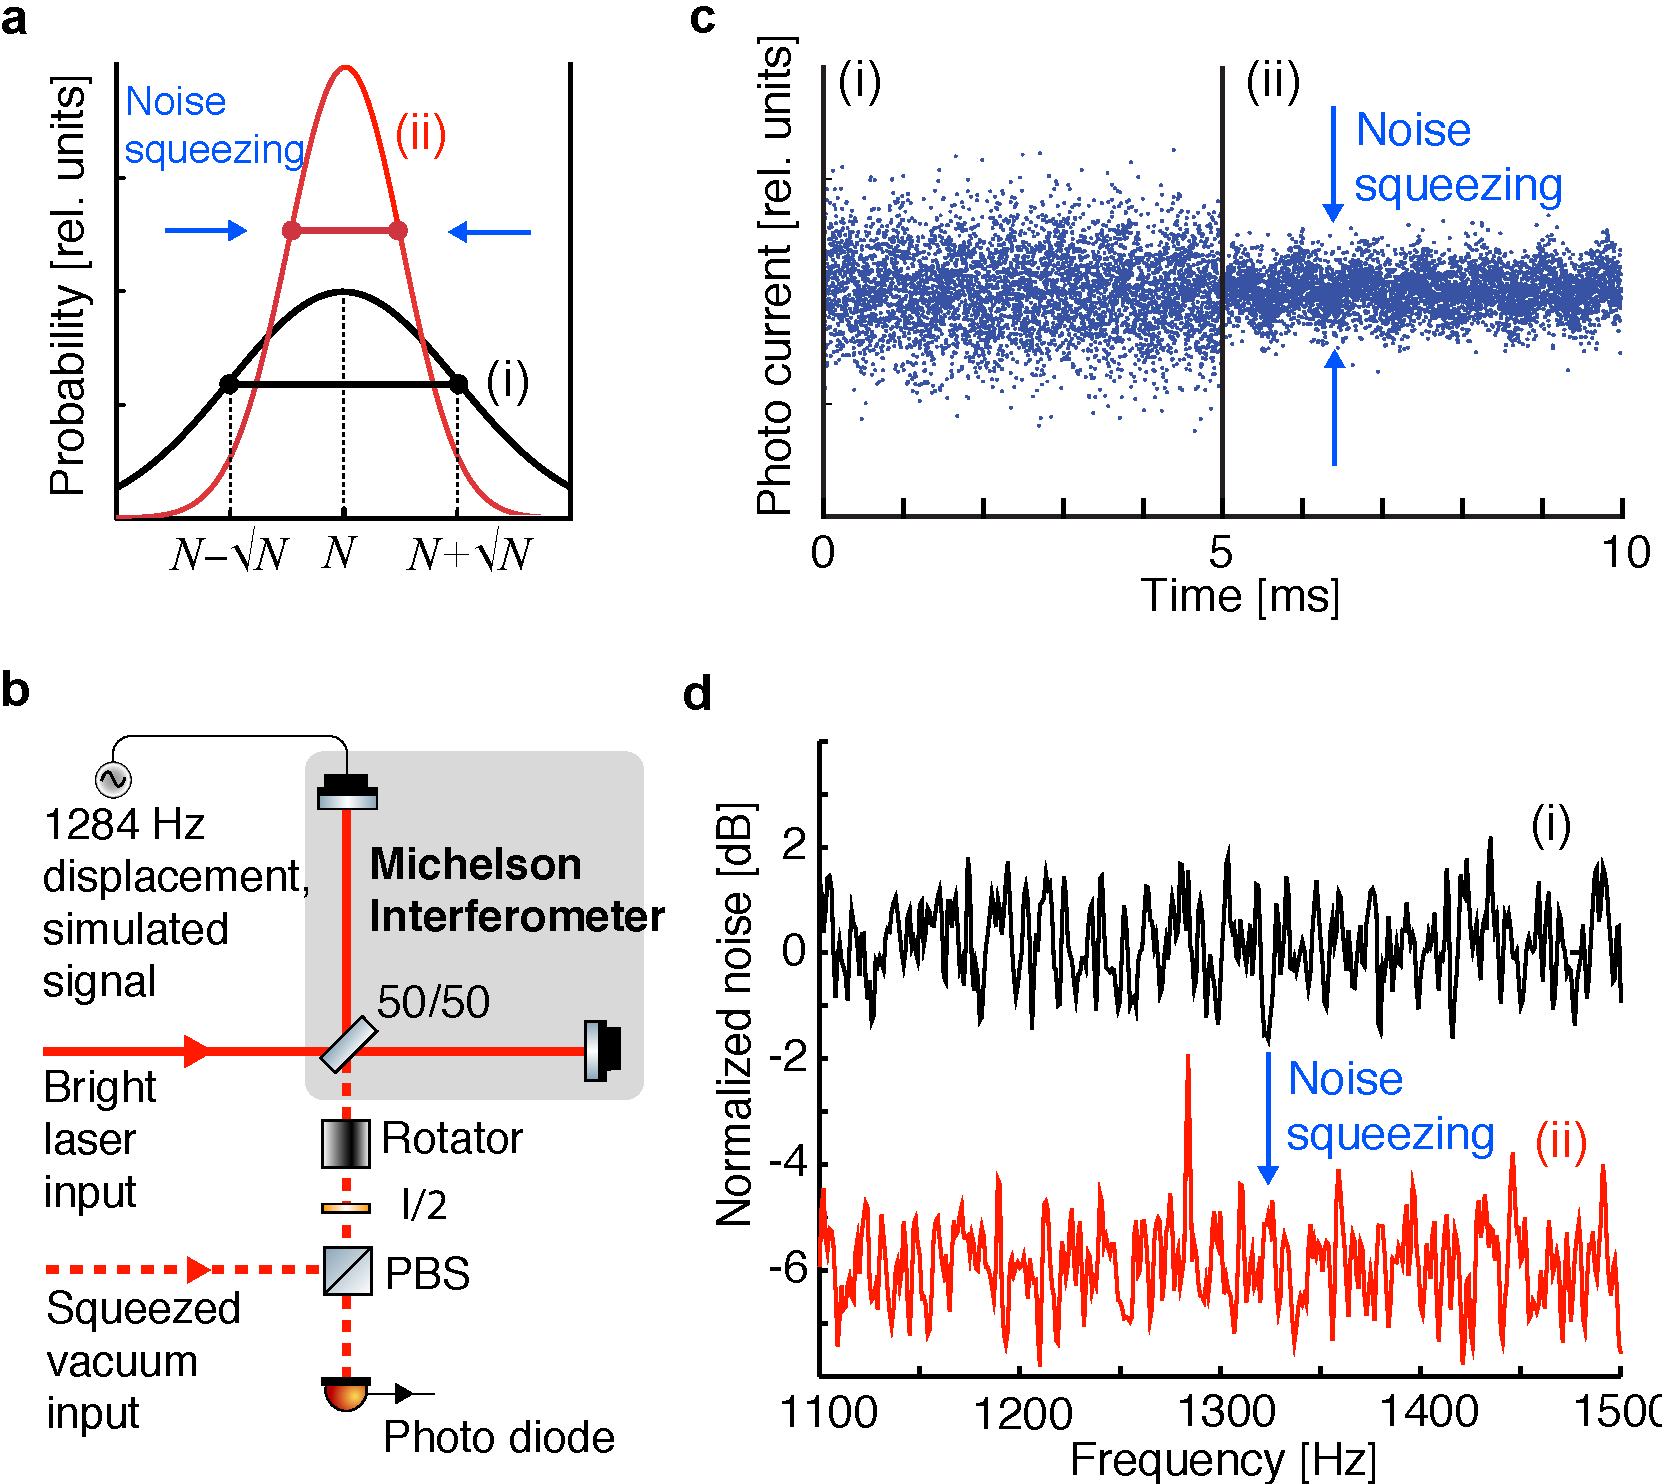
\includegraphics[scale=0.42]{./Sec_Optics/SqzIllustration.pdf}
\caption[Squeezed light enhanced metrology]{{\textbf{Squeezed light enhanced metrology} \; (a) For large photon numbers $N$, squeezed light shows a photon counting statistic with a standard deviation smaller than $\pm \sqrt{N}$. In all panels, (i) correspond to shot-noise and (ii) to 6\,dB squeezed noise. (b) A squeezed vacuum beam is injected into the dark signal port of a Michelson interferometer, in addition to the conventional bright laser input. The squeezed beam leads to path entanglement of the light fields in the two arms and to an improved signal to noise ratio, as shown on the right. Without squeezing, the optical path length modulation at 1284\,Hz is neither visible in the time series of the photo-electron current (c, simulation by B. Hage, AEI) nor in its noise power spectrum (d, measurement, courtesy of H. Vahlbruch, AEI \cite{VahlbruchPhD08}). In (c) as well as in (d), the signal is clearly visible when squeezing is applied (ii).}
}\label{fig:SqzIll}
\end{figure}%
}



Squeezed states \cite{Yuen1976,Walls1983,Breitenbach1997,Dodonov2002} belong to the class of so-called \textit{nonclassical} states of light.
Generally, nonclassical states are those that cannot be described by a classical (positive valued) probability distribution using the coherent states as a basis (the $P$-representation) \cite{GerryKnight}. Let us first consider the coherent states. If light in a coherent state is absorbed by a photodiode, mutually independent photon `clicks' (in terms of photo-electrons) are recorded, a process that is described by Poissonian counting statistics. Due to quantum mechanics, every individual `click' is not predictable, but rather the result of a truly random process. If the number of photons per time interval is large ($N\!>\!\!>\!1$), its standard deviation is given by $\sqrt{N}$, see Fig.~\ref{fig:SqzIll}\,a\,(i). This uncertainty gives rise to \textit{shot-noise}. For a \emph{squeezed} light beam, the detection of photons is not time-independent but instead contains quantum correlations.  Nevertheless, the photon statistics still cannot be predicted by some external clock. It instead shows auto-correlations that give rise to a reduced standard deviation, as shown in Fig.~\ref{fig:SqzIll}\,a\,(ii). The correlations might be described in the following way. Whenever the quantum statistics might drive the actual photon number above the average value $N$, a similar number of photons destructively interfere with the main body of photons providing a (partial) compensation of the fluctuation. These quantum correlations \textit{squeeze} the interferometer's shot-noise below its natural value. Another complementary way of describing the properties of squeezed states is based on the phase space quasi-probability distribution using the amplitude and phase quadratures of a light wave (the Wigner function) \cite{Walls1983,GerryKnight}.

A squeezed state that contains only quantum-correlated photons with no coherent amplitude is called a \textit{squeezed vacuum state} \cite{GerryKnight}. If such a state is overlapped with a coherent laser beam on a semi-transparent beam splitter, two beam splitter outputs are generated which are quantum correlated. As a consequence, the overall (bi-partite) quantum state cannot be written in terms of products of the two beam splitter output states. Such a quantum state is called non-separable or \textit{entangled}. This is exactly what happens if a squeezed state is injected into the signal output port of a laser interferometer for GW detection (Fig.~\ref{fig:SqzIll}\,b). The two \textit{high-power} light fields in the interferometer arms get entangled and the light's quantum fluctuations in the two arms are correlated with each other. Although the fluctuations are not predictable from the outside, they provide an improved signal-to-noise ratio in the interferometer. Recall that an interferometer measures the optical path length change in one interferometer arm with respect to the other arm. If the quantum noise in the two arms is correlated it will cancel out.
This entanglement interpretation was not discussed in the initial proposal by Caves.  Nevertheless, it shows that the application of squeezed states in interferometers is a real application of quantum metrology by its very own definition. The entanglement produced by splitting a squeezed state at a semi-transparent beam splitter was tomographically characterized and quantified in \cite{DiGuglielmo2007}. Fig.~\ref{fig:SqzIll}\,c shows a simulated signal from a photodiode, without (i) and with (ii) \textit{squeezing}. The tiny modulation in the interferometer's output light due to the (simulated) passing GW is visible only with the improved signal-to-noise ratio. Fig.~\ref{fig:SqzIll}\,d shows the analogue in frequency space, i.e.\ after a Fourier transform of the photo current was applied.

The above paragraph shows that squeezed states can be conveniently combined with the extremely
high photon numbers of coherent light to improve a laser interferometer, as proposed in \cite{Caves1981}
and shown in Fig.~\ref{fig:SqzIll}\,b. In fact, the stronger the squeezing
factor \cite{Walls1983,GerryKnight} the greater the path entanglement and the signal-to-noise
improvement. %Very strong path entanglement is present in interferometers using so-called NOON-states instead of squeezed states.  NOON states are another class of nonclassical states \cite{GerryKnight04,HBu93,WPAUGZ04,AAS10}.   Unfortunately, the strong entanglement of a NOON state is extremely fragile, in particular if $N$ is large. Very recently a NOON-state with $N=5$ photons was demonstrated \cite{AAS10}. However, gravitational wave detectors use coherent high-power laser light with $N \approx 10^{23}$ photons per second. An improvement by use of NOON states is, therefore, far out of reach.

%\textcolor{red}{Overlap with Sec.~\ref{subsec:qnft}}.

Shortly after Caves proposed squeezed states of light for laser
interferometers in 1981, the first experimental demonstration of squeezed
light \cite{Slusher1985} and proof of principle demonstrations of
quantum metrology were achieved \cite{Xiao1987,Grangier1987}. In parallel, it was theoretically discovered that squeezed states offer even more advances in metrology than `just' reducing the quantum shot-noise.
From the early days of quantum physics, when fundamental
aspects of the measurement process were discussed, it was clear that,
in general, a measurement disturbs the system to be measured
\cite{Braginsky1999}. %Braginsky95}.
 The measurement of quantity $A$ (say
a position of a mirror) increases the uncertainty of the
non-commuting quantity $B$ (say the mirror's momentum). Both
observables are linked by a Heisenberg Uncertainty relation. For
repeated measurements of $A$, the increased uncertainty in $B$
disturbs the measurement of $A$ at later times. This is referred to
as \textit{quantum back-action noise}. Here, the back-action arises
from the fluctuating radiation pressure due to the reflected light \cite{CavesPRL451980}.
It is significant if the mirror's mass is low and a
large photon number is reflected. In the 1970s, ideas were developed
that showed how, in principle, back-action noise for continuous
measurements can be avoided. Such schemes were called
quantum-non-demolition (QND) measurements \cite{Thorne1978, BraginskyRMP1996}.
However, for laser interferometric GW detectors
using \textit{quasi-free} falling mirrors it remained unclear if QND schemes
exist. In \cite{CavesPRL451980,Caves1981} it was concluded that back-action noise
of a free mass position measurement can in principle not be avoided and, together with photon counting noise, defines a \textsl{standard
quantum limit} (SQL). In \cite{Yuen1983,Unruh1983} it was argued, however, that measurements below the
SQL of a free mass are indeed possible. The discussion
remained controversial \cite{CavesPRL1985} until Jaekel and Reynaud
\cite{Jaekel1990} were able to convincingly show that the cleverly
arranged squeezed states in a GW detector can simultaneously reduce
the shot-noise and the radiation pressure noise, by almost arbitrary
amounts (as long as most of the photons belong to the light's coherent displacement).
%\textcolor{red}{Refer to Sec.~\ref{subsec:qnft}, great overlap, arrange Secs properly... }

So far no experiment has achieved a position measurement with
sensitivity even at, let alone below, its standard quantum limit.
Eventually this will be achieved, possibly first in future
gravitational wave detectors.  Advanced detectors are in
fact designed to have a sensitivity at or just below their SQLs.
Once the SQL is reached, a new level of quantum metrology is achieved, because the position-momentum
uncertainty of the mirror becomes correlated with the quadrature
uncertainty of the reflected optical field. In this way, entanglement
between the mechanical and the optical system can be observed
\cite{Vitali2007}. This is all the more remarkable from the perspective of GW detectors
since we are talking about mirrors with masses of 40 kg, planned for
the upcoming Advanced LIGO \cite{aLIGO}, and even in the order of a 100\,kg concerning the envisaged LF-detector of ET.
Eventually, even two such mirrors might be projected via entanglement swapping
\cite{Pirandola2006} into an entangled state \cite{M-Ebhardt2008}.
Obviously quantum metrology opens the possibility for further
studies of the peculiarities of quantum physics at a macroscopic scale.



\FloatBarrier
\paragraph{Squeezed light for Gravitational wave astronomy}\label{subsec:SQZforGWD}
Laser interferometers for GW astronomy are facing extreme sensitivity requirements that can only be achieved if all available
tools, inclusive of quantum metrology, are combined in an elaborate measurement device.  Squeezed light must be generated in a non-linear
interaction. Squeezed light was first produced in 1985 by
Slusher et al.\ using four-wave-mixing in Na atoms in an optical
cavity \cite{Slusher1985}. Shortly after, squeezed light was also
generated by four-wave-mixing in an optical fibre \cite{Shelby1986}
and by parametric down-conversion in an optical cavity containing a
second order non-linear material \cite{Wu1986}. In these early day
experiments, squeezing of a few percent to 2  to 3\,dB were routinely observed (For an
overview of earlier experiments and squeezed light generation in
the continuous-wave as well as pulsed regime please refer to Ref.~\cite{BachorRalph2004}).


\begin{figure}[ht]
  \centering
  \includegraphics[scale = .41]{./Sec_Optics/SqzGen.pdf}
  \vspace{-1mm}
\caption{{\textbf{Generation of squeezed light} (a) A continuous-wave laser beam at the GW detector wavelength is first spatially filtered and then up-converted to a field at half the wavelength (second harmonic generation, SHG). That beam is then mode-matched into the `squeezing resonator' in which a tiny fraction of the up-converted photons are spontaneously down-converted by optical parametric amplification (OPA) producing a squeezed vacuum state. The squeezing factor is validated by a balanced homodyne detector (BHD). SHG as well as OPA are realized by a non-linear crystal (b), here a 6\,mm long MgO:LiNbO$_3$ crystal, inside an optical resonator (c) formed by an external cavity mirror and the dielectrically coated crystal back surface. The two non-linear resonators may be constructed in an identical way and are put into temperature stabilized housings (d).}
}
\label{fig:SqzGen}
\end{figure}

GW detectors are operated with high-power, quasi-monochromatic
continuous-wave laser light with an almost Fourier-limited spatial
distribution of a Gaussian TEM$_{00}$ mode. For a non-classical
sensitivity improvement, squeezed light in exactly the same
spatio-temporal mode must be generated and mode-matched into the
output port of the interferometer \cite{Caves1981}, providing
interference with the high-power coherent laser beam at the
interferometer's central beam splitter. High-power lasers for GW
astronomy are based on optically pumped solid-state crystals in
resonators \cite{Frede2006}%\textcolor{red}{refer to sec 'Pre-stabilized laser'}
, suggestive of a similar configuration for
a ``squeezed light resonator''. Fig.~\ref{fig:SqzGen}\,(a) shows a
schematic setup for generation of squeezed light that is built upon one of the very first squeezing experiments \cite{Wu1986}, a setup that has been used in many experiments thereafter
\cite{Furusawa1998,Bowen2003,Schneider1998,Lam1999}. The setup uses a solid
state laser similar to those used as master lasers in high-power
systems. After spatial mode filtering, second harmonic
generation (SHG) in an optical cavity containing a second-order
non-linear crystal is applied to produce laser light at twice the
optical frequency. The second harmonic light is then mode-matched
into the squeezing resonator to pump a degenerate optical parametric amplifier.

Fig.~\ref{fig:SqzGen}\,(b-d) show photographs of the non-linear crystal, the optical arrangement and the housing of a squeezing resonator. The crystal is temperature-stabilized at its phase-matching temperature. At this temperature the first-order dielectric
polarization of the birefringent crystal material with respect to the pump is
optimally overlapped with the second-order dielectric polarization of
the resonator mode at the fundamental laser frequency. This ensures
a high energy transfer from the pump field to the fundamental
Gaussian TEM$_{00}$ resonator mode, i.e.\ efficient parametric down
conversion.

Initially, the resonator mode is not excited by photons
around the fundamental frequency, i.e.\ it is in its ground state,
characterized by vacuum fluctuations due to the zero point energy
\cite{GerryKnight}. Note that the process is typically operated
\textit{below} oscillation threshold in order to reduce phase noise coupling
from the pump \cite{Reid1989}.  This setup produces a squeezed vacuum
state \cite{GerryKnight}. The down-converted photon pairs leaving the squeezing
resonator exhibit quantum correlations which give rise to a squeezed
photon counting noise when overlapped with a bright coherent local
oscillator beam. The squeezed field is detected by interfering it
with a coherent local oscillator beam, either in a balanced homodyne
detector (BHD), see Fig.~\ref{fig:SqzGen}\,(a), or when injected into a GW
detector and detected with a local oscillator from the GW detector
along with an interferometric phase signal, see Fig.~\ref{fig:SqzIll}. The closer
the squeezing resonator is operated to its oscillation threshold,
and the lower the optical loss\footnote{In this context the term optical
loss refers to the total power loss experienced by the squeezed light from the squeezed light source to the photo 
detector.} on down-converted photon pairs, the
greater the squeeze factor is. For instance, the observation of a
squeezing factor of 2
is only possible if the
overall optical loss is less than 50\%~\cite{BachorRalph2004}. A
90\% nonclassical noise reduction, i.e.\ a squeezing factor of 10, or
10\,dB, already limits the allowed optical loss to less
than 10\%.

Although squeezed light was demonstrated in the 1980s
shortly after the first applications were
proposed \cite{Slusher1985,Shelby1986,Wu1986}, several important challenges pertaining to the application of
squeezed states to GW detectors remained unsolved until recently.

First, squeezing has always been demonstrated at megahertz
frequencies, where the technical noise of the laser light sources is not present.  At these frequencies, the laser operates at or near the shot-noise limit.  In the 10\,Hz to
10\,kHz band where terrestrial GW detectors operate,
technical noise masked and overwhelmed the observation of squeezing.  For example,  thermal and mechanical 
fluctuations can be many orders of magnitude larger than shot noise.
Until recently, it was not certain that a laser field could even be squeezed and matched to the
slow oscillation period of GWs.
Second, it was previously not known whether squeezed light was fully
compatible with other extremely sophisticated technologies employed
in GW detectors, such as signal-recycling.
Third, the technology to reliably produce stable and strong
squeezing with large squeeze factors was lacking.  Long term observation of strong squeezing was a technical challenge until recently.

These challenges have all been overcome in the past decade.  All the open questions have now been satisfactorily addressed.  This development is very timely since many known advanced classical interferometric techniques have almost been exhausted.  Many remaining classical improvements are becoming increasingly difficult and expensive to implement.

\begin{figure}
\centering
 \includegraphics[scale=.45]{./Sec_Optics/SqzAudioNew.pdf}
\caption{\textbf{Quantum noise squeezing}\; The spectral analysis of measured noise powers without\,(a) and with `squeezing'\,(b). Trace (a) is the 'non-squeezed' shot-noise, serving as reference level (0\,dB). The corresponding noise in the orthogonal quadrature, 'anti-squeezed', is shown in trace\,(c). Trace\,(d) shows the electronic dark noise level. Current best performance of a squeezed light laser for GW detection shows an up to 9\,dB squeezed noise over the complete detection band of ground-based GW detectors~\cite{VahlbruchCQG2010}.}
\label{fig:SqzAudio}
\end{figure}



\paragraph{Generation of squeezing in the audio-band}\; A major
breakthrough in achieving squeezing in the audio band was the
insight that the dominant noise at audio frequencies that
degrades squeezed light generation couples via the coherent laser
field that was used to control the length of the squeezed light
laser resonator, whereas noise coupling via the second harmonic
pump field is insignificant \cite{Bowen2002,Schnabel2004}. This led
to the first demonstration of audio-band squeezing at frequencies
down to 200\,Hz \cite{McKenzie2004}, see Fig.~\ref{fig:SqzAudio}\,a. There the length of the squeezing
resonator was stabilized without a bright control beam by using the phase sensitivity of the squeezing itself---a technique known as quantum noise locking~\cite{McKenzie2005}. Subsequently a coherent beam control scheme was invented \cite{Vahlbruch2006} for simultaneous control of both the squeezing resonator length and the squeezing angle \cite{GerryKnight}. Shortly thereafter another noise source was
identified and mitigated, which allowed for squeezing of more than
6\,dB throughout the audio-band down to 1\,Hz \cite{Vahlbruch2007}. This
noise source arose due to tiny numbers of photons that were
scattered from the main laser beam and rescattered into the audio
band squeezing mode after having experienced a frequency shift due
to vibrations and thermal expansions of potential scattering
surfaces, an effect known as \textit{parasitic interferences}. Since
bright laser beams cannot be completely avoided, the recipe for the
generation of audio-band squeezing turned out to be fourfold:
avoiding scattering by using ultra-clean super-polished optics,
avoiding rescattering by carefully blocking all residual faint beams
caused by imperfect anti-reflecting surfaces, reduce the
vibrationally and thermally excited motion of all mechanical parts
that could potentially act as a re-scattering surface and avoid pointing fluctuations \cite{McKenzie2007}.

\paragraph{Compatibility of squeezing with other interferometer techniques}\; Current detectors achieve their exquisite
sensitivity to GWs due to their kilometre-scale arm lengths, the
enormous light powers circulating in the enhancement resonators
(arm, power- and signal-recycling cavities),
and sophisticated pendulum suspensions that isolate the test mass
mirrors from the environment %(Fig.~\ref{fig3}).
When these
techniques were developed, squeezing was not envisioned to become an
integrated part of such a system. Building on existing theoretical
work \cite{Gea-Banacloche1987,OpticalSpringHarms2003}, a series of experimental demonstrations
of squeezed state injection into GW detectors were carried out.
These included compatibility with power recycling, with signal
recycling \cite{McKenzie2002,Vahlbruch2005}, and with the dynamical system of
suspended, quasi-free mirrors \cite{Goda2008,Schnabel2008}.


\paragraph{Generation of strong squeezing}\; Squeezing has significant
impact in quantum metrology if large squeezing factors can be
produced. Squeezing of 3\,dB improves the signal-to-noise ratio by a
factor of $\sqrt{2}$, equivalent to doubling the power of the
coherent laser input. Squeezing of 10\,dB corresponds to a ten-fold
power increase. Remarkably, the experimentally demonstrated
squeezing factors have virtually exploded in recent years
\cite{Takeno2007,Vahlbruch2008,Polzik2008}, culminating in values
as large as 12.7\,dB \cite{Eberle2010}.
All the squeezing factors above
10\,dB were observed with monolithic resonators and at MHz
frequencies. However, reduced optical loss in non-monolithic resonators and a careful elimination of
parasitic interferences should in principle enable such factors
also in the GW band.  An 8 to 10\,dB improvement based on strong squeezing seems
realistic for future GW detectors in their shot-noise limited band \cite{Eberle2010}.

So far, strong squeezing values have been reported for a wavelength of 1064\,nm. However, the procedure of squeezed light generation is also applicable for the wavelength of 1550\,nm that will be required for future, cryogenic GW detectors.
Recently, the generation of  squeezing at a wavelength of 1550\,nm  was reported in a first proof-of-principle experiment~\cite{Mehmet2009}.


\paragraph{The first squeezed light laser for GW detection}\; Based on
the previous achievements reviewed here, very recently the first
squeezed light laser for continuous operation in GW detectors was
designed and completed \cite{VahlbruchPhD08,VahlbruchCQG2010}. Up to
9\,dB of squeezing over the entire GW detection band have been
demonstrated (Fig.~\ref{fig:SqzAudio}b). This laser produces squeezed vacuum
states and is fully controlled via co-propagating frequency-shifted bright control
beams. This 9\,dB squeezing factor is limited by technical effects:
the squeezing resonator has to have an adjustable air gap to allow
for an easy way to apply length control. The anti-reflection coated surface
in the resonator introduces additional loss and reduces the escape
efficiency. Moreover, a Faraday isolator has to be used in the
squeezed beam path in order to eliminate parasitic interferences.
This rotator produces a single pass photon loss of about 2\%. This
squeezed light source is designated for continuous operation in the
GEO600 GW detector. A squeezed light source based on a design that should have less sensitivity to retro-scattered light \cite{McKenzie2006} is being prepared for deployment on one of the most sensitive
detectors, the 4\,km LIGO detector in Hanford, Washington.

\FloatBarrier
\begin{figure}[H]
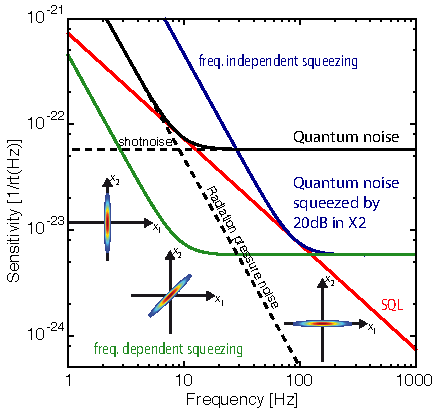
\includegraphics[width =0.5\textwidth]{./Sec_Optics/MI_SQL_AI.pdf}
\hspace{35pt}
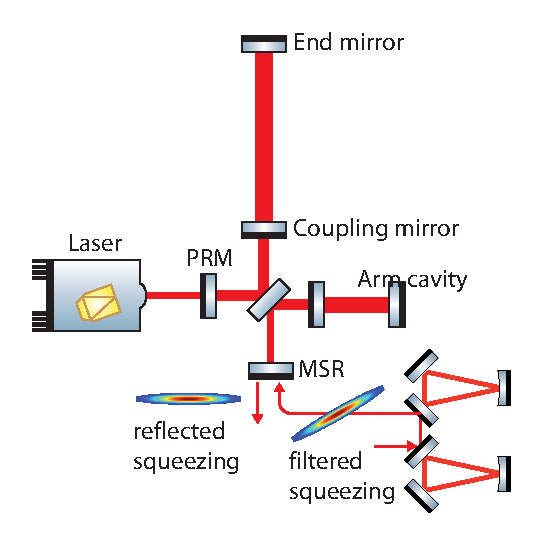
\includegraphics[scale=0.8]{./Sec_Optics/FilterMI-Ill_v2.pdf}
\caption[Illustration of frequency dependent and independent squeezed light injection]{Beating the SQL in position meter with frequency dependent light (left). Injection of frequency dependent squeezed light injection in an optical spring interferometer (right).} \label{fig:FilterMI-Ill}
\end{figure}
\subsubsection{Filter cavities}\label{sec:filtercavities}
At first view the enhancement of an interferometer's sensitivity with frequency independent squeezing (squeezed light with a fixed quadrature angle) can only be achieved in a certain frequency range. This is a direct consequence of the Heisenberg uncertainty principle. Considering a simple Michelson interferometer the quantum noise in its phase quadrature (shot noise) can be reduced by the amount of squeezing. Unfortunately, the quantum noise in the amplitude quadrature (radiation pressure noise) will be increased by the same amount enhancing the noise at low frequencies.
 
It was revealed by Unruh~\cite{Unruh1982} and others~\cite{Yuen1983, Pace1993} that squeezed field injection with frequency dependent squeezing angle allows an overall quantum noise reduction including the radiation pressure noise thereby beating the standard quantum limit (SQL). This is demonstrated in Fig.~\ref{fig:FilterMI-Ill} (left).
Figure~\ref{fig:FilterMI-Ill} (right) illustrates squeezed light injection in an optical spring interferometer. Here, an additional rotation of the squeezing ellipse is caused first by the phase-space rotation of a detuned cavity and second due to the optical spring resonance. In this case at least two filter cavities are necessary to achieve a broadband reduction of quantum noise with squeezed states of light. This is what we propose for the low-frequency ET-LF interferometer (cf. Sec.~\ref{sec:xylophone}). For the high-frequency ET-HF interferometer one filter cavity is enough (cf. Sec.~\ref{sec:xylophone} and \cite{Hild2010b}). Details about the derivation of the filter cavities design parameters are given in Appendix~\ref{app:detfcparams}.

Figure~\ref{fig:WigIll} shows the Wigner representation of a coherent vacuum state and a 20\,dB squeezed state for different squeezing angles.
\begin{figure}[H]
\centering
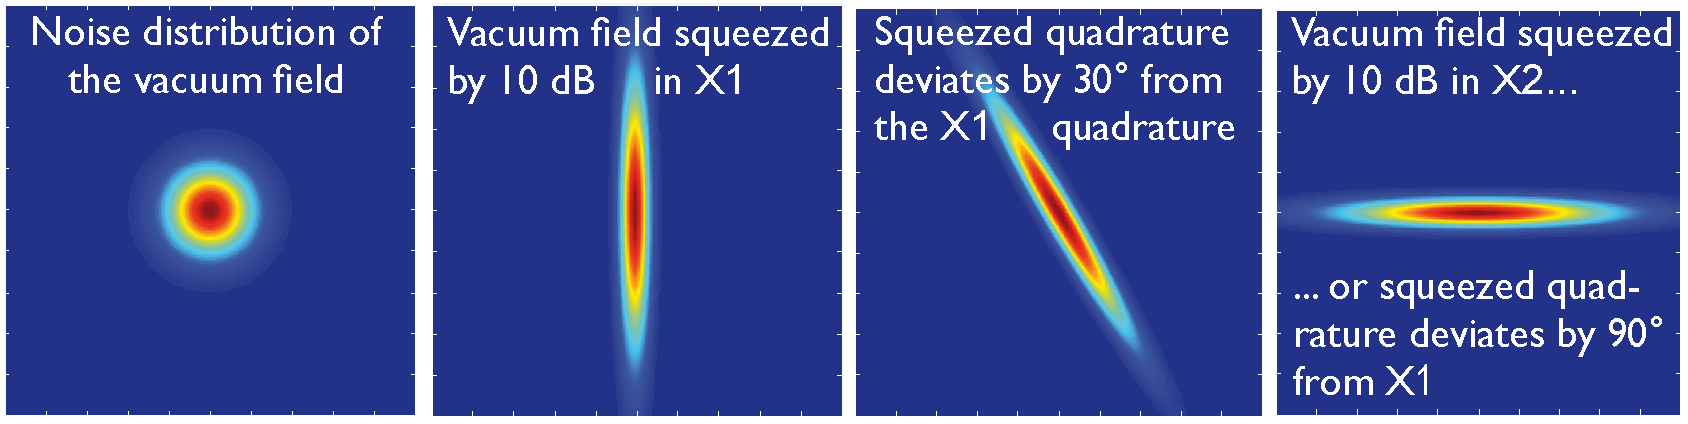
\includegraphics[width=0.7\textwidth]{Sec_Optics/WigSqzIll.pdf}%\hspace{10pt}
\caption[Wigner representation of squeezed states ]{From left to right: Wigner representation of a vacuum state (left), a pure 10\,dB amplitude squeezed state, a 10\,dB squeezed state rotated in phase-space by 30 degrees and an amplitude squeezed state rotated by 90 degrees, i.e.\ a phase squeezed state.}
\label{fig:WigIll}
\end{figure}

\FloatBarrier
\paragraph{Restrictions for the baseline length of the filter cavity}
According to the laws of quantum mechanics, whenever the optical losses (like scattering, absorbtion, etc) are encountered in the optical train, the light in the vacuum state is introduced. This generally unsqueezed light mixes up with the squeezed light thus lowering the squeezing factor of the latter. This is usually referred to as the degradation of the squeezed state which leads to the decrease of sensitivity. We demonstrate this degradation schematically in Fig.~\ref{fig:sqz-vs-loss-ill} and show dependence of the squeezing factor on the losses in Fig.~\ref{fig:sqz-vs-loss-chart}.
\begin{figure}[H]
\centering
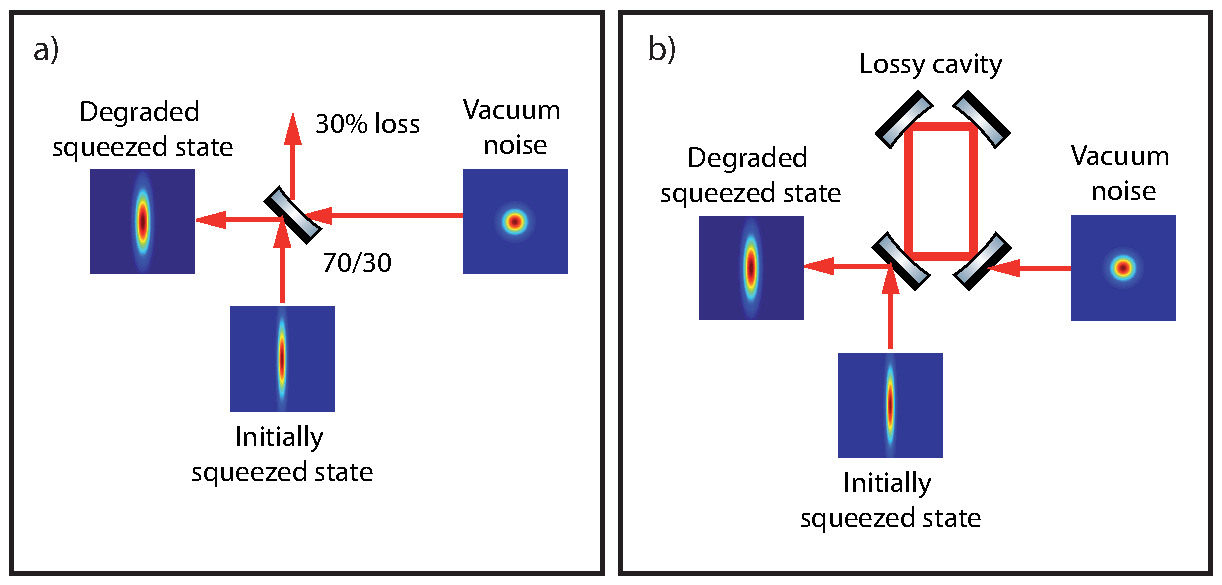
\includegraphics[scale = .6]{./Sec_Optics/Sqz-vs-loss.pdf}
\caption[Intermixture of vacuum noise to a squeezed field at lossy optics]{The figure illustrates the intermixture of vacuum noise to a squeezed field at lossy (open) ports. a) Consideration of a beam splitter  with {$R_{\rm bs} = \rho_{\rm bs}^2 = 0.7$} and {$T_{\rm bs} = \tau_{\rm bs}^2 = 0.3$}. In reflection of the beam splitter the initially squeezed state gets attenuated by the factor $\rho_{\rm bs}$. The vacuum noise couples to the reflected squeezed field with an efficiency of $\tau_{\rm bs}$ leading to a degradation of the squeezing level. b) Consideration of a lossy cavity. In this case, the intermixture of vacuum noise is frequency dependent, since the transfer function of the cavity comes into play. The degradation is maximum at the resonance frequency of the cavity. At frequencies far away from resonance the cavity behaves like an almost perfect mirror, i.e.\ the squeezing is preserved.} \label{fig:sqz-vs-loss-ill}
\end{figure}
\begin{figure}[ht]
\centering
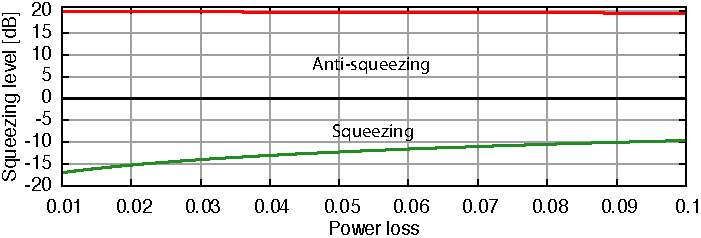
\includegraphics[scale = 1]{./Sec_Optics/SQZ-20dB-losschartAI-ill.pdf}
\caption[Degradation of a 20\,dB squeezed state due to optical loss]{The figure shows the degradation of a 20\,dB squeezed state due to optical loss. It can be seen that in contrast to the anti-squeezing level, the squeezing degrades rapidly with increasing loss. At a power loss of about 9\,\% the squeezing level is reduced from 20\,dB to 10\,dB whereas the anti-squeezing level is still about 19.6\,dB.} \label{fig:sqz-vs-loss-chart}
\end{figure}


Generally, any round-trip loss will degrade the squeezing level at
sideband frequencies being resonant in the filter cavity. For a
given power round-trip loss (mainly caused by
scattering) the resulting loss in reflection of the filter cavity
increases with a decreasing baseline length of the
filter. As well, for a certain length and a certain
round-trip loss the loss imposed on the squeezed
field increases with a decreasing half-bandwidth
that needs to be realized. The details about determination of the baseline length are given in Appendix~\ref{app:FClength}. Figure~\ref{fig:length_maintext} shows the filter cavity performance as a function of its baseline length.
\begin{figure}[ht]
\centering
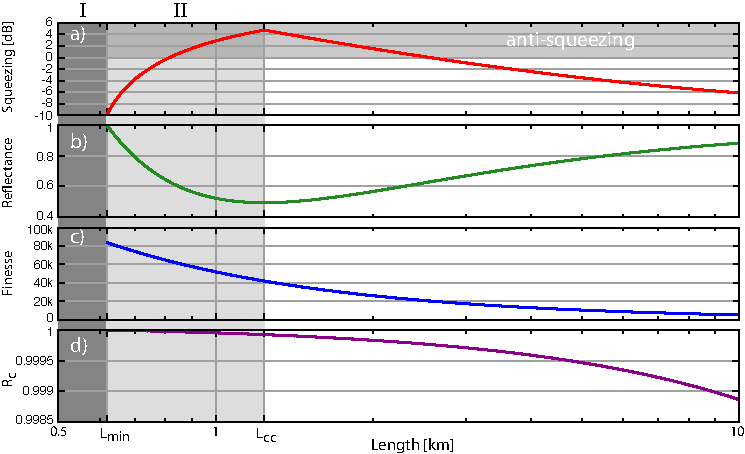
\includegraphics [scale = 1.1]{./Sec_Optics/FCslength75ppmAI.pdf}
\caption{The figure shows the filter cavity performance as a function of its baseline length $L_{\rm fc}$ (details in Appendix~\ref{app:FClength}). Graph~a) shows the remaining squeezing level in reflection of the filter cavity at its resonance frequency. Graph~b) shows the according  reflectance of the filter cavity. Graph~c) and d) show the filter cavity finesse and coupling mirror reflectance $R_{\rm c}$, respectively. The two grey shaded areas in the left highlight the region where $L_{\rm fc}<L_{\rm cc}$ (area II) and where $L_{\rm fc}<L_{\rm min}$ (area I). In the considered example ($\gamma_{\rm fc} =2\pi\cdot1.4\,{\rm Hz}$, $\Phi_{\rm fc_1}= 2\pi\cdot6.6\,{\rm Hz}\cdot L_{\rm fc_1}/c$,  $l^2_{\rm rt,fc}=75\,{\rm ppm}$) the critical length $L_{\rm cc}$ is about 1239\,m. The top grey shaded area in graph a) highlights the anti-squeezed region. Due to the unbalanced loss for upper and lower squeezing sidebands in the detuned filter cavity, for high resulting loss (i.e.\ for a cavity reflectance much smaller than one) the detected noise can be enhanced even when compared to the vacuum noise (refer to Fig.~\ref{fig:phasediffusedSQZ}). In the considered example the detected noise is already enhanced (anti-squeezed) for filter cavity baseline lengths smaller than approximately 2.5\,km.}
\label{fig:length_maintext}
\end{figure}

Our investigation demonstrated that the round-trip loss ultimately restricts the minimal allowed baseline length and consistently the performance of the filter cavities. As it is expected that the round-trip loss of the filters will be dominated by scattering at imperfect mirror surfaces, the optical layout needs to be designed such that the amount of scattering is reduced as much as possible. The scattering in different optical layouts is treated in below.
Figure~\ref{fig:sensETDHF} demonstrates the sensitivity of the ET-D-HF interferometer at various lengths of the filter cavities. Note that the high-frequency sensitivity is mostly independent of the cavity length while the low-frequency one decreases with the decrease of length.
\begin{figure}[ht]
\centering
\includegraphics{./Sec_Optics/ET-D-HF-FCs.pdf}
\caption{Sensitivity curves for ET-D-HF assuming various lengths for the filter cavity. Parameters used: round-trip loss 75ppm, 9\% frequency independent propagation loss, pure 20dB squeezing injected.}
\label{fig:sensETDHF}
\end{figure}

%%% Removed adf 27.04.2011 as the text is not complete
\begin{comment}
\longetbox{i}{box:FCdevbw}{The effect of a deviating bandwidth}{
Rotation in the wings of the FCs resonance not compensated for, thus not optimally squeezed or even enhanced noise (when compared to shot noise...
\begin{figure}[H]
\centering
\includegraphics{./Sec_Optics/FCi-devbw_reviewAI.pdf}
\caption{The figure shows the squeezing spectra for a deviation of the designed bandwidth of a) the single FC$_1$  and b) the single FC$_2$. Graph c) shows the spectra if both  filter cavities are considered. In all cases, the filter cavity round-trip loss was considered to be 75\,ppm.}
\label{fig:devBW}
\end{figure}}
\end{comment}

\paragraph{Robustness of filter cavity design parameters}
The most obvious quantities, that will potentially  change the properties of the filter are: the reflectance factors of the used mirrors, the round-trip loss, the macroscopic length, and the resonance frequency.

The first three quantities affect the bandwidth of the filter cavity and thus the required phase-space rotation around the targeted resonance frequency. A deviation from the design values of these quantities could not be compensated if the filter cavity is realised as a single resonator. An adaption of the filters bandwidth would be possible if coupled resonators---e.g.\ a linearly coupled three-mirror cavity---are utilised.  Although it should be always possible to tune the filter cavity to the required resonance frequency, for the sake of completeness we treat a potential mismatch (see details in Appendix~\ref{app:robustparam}). From the results, the requirements for the length stabilisation with regard to displacement noise could be determined. 
If a tolerable  degradation  of the squeezing  by less than 2\,dB (related to the squeezing levels  achievable with  the  design parameters) is targeted, a deviation of the bandwidth less than 5\,\% is acceptable. From this value, the tolerances for the design parameters can be deduced. 

\FloatBarrier
\begin{figure}[htb]
\centering
\includegraphics[width=0.5\textwidth]{./Sec_Optics/cavity-designs.pdf}
\caption{Four geometries were analysed from the scattering point of view.}
\label{fig:sc_geometry}
\end{figure}
\paragraph{Choosing the optical layout of the filter cavity}\label{subsec:fcscattering}

%\emph{Author(s): K. Kokeyama, A. Freise, H. L{\"u}ck}

The Einstein Telescope required two 10\,km long and one comparatively
short (several hundred meters long) filter cavities per detector. 
Such filter cavities provide the correct frequency dependence for the injected squeezing state
in order to obtain broad band quantum noise suppression in the main interferometer.
The light reflected off these cavities needs to be injected into the
interferometer dark ports. In principle any cavity geometry can 
provide the correct filtering, however, practical concerns will 
put constraints on the geometry. %In this section we briefly discuss
%these issues, while a selection of the cavity geometry has not been done at this stage.
The four cavity geometries depicted in Fig.~\ref{fig:sc_geometry} are
possible candidates;
the following advantages and disadvantages follow directly from the
geometry (given a long baseline):
\begin{itemize} 
\item the 2-mirror cavity has the advantage of using only two mirrors but
  in order to extract the reflected beam, polarising optics are
  required which introduce additional optical losses and phase noise
\item the 3-mirror cavity provides the reflected beam without the need
  for extra optics. However, the small angle between the beams at the
  far right mirror means that the setup is more sensitive to small
  angle scattering, a problem which has been seen for example in the
  triangular input mode cleaner cavity of VIRGO. Another problem is
  that the large angle of incidence on the two left mirrors requires
  the mirrors to be significant larger compared to the 2-mirror setup.
  of the 10\,km long linear arm cavities. Since the ET optical design is 
  assuming the largest available mirrors being used for the linear arm cavity, this filter
  cavity geometry can be excluded. 
\item the rectangular 4-mirror setup also has the problem of requiring
  larger mirrors due to the angle of incidence.
\item The bow-tie cavity can separate the reflected beam from the
  injected one and does not feature large angles of
  incidence so that the mirror sizes are similar to those of a linear cavity. However, it 
  is sensitive to small angle scattering.
\end{itemize}

% motivation

A detailed study of scattering in the main interferometer and the
filter cavities has not been done yet. 
In Appendix~\ref{app:scatter} we provide a first analysis of the
amount of scattering between the suspended optics itself and conclude
that this effect can be ignored in the selection of the cavity geometry. 






% memo
% mirror surface and scattering
% BRDF
% 4 topologies were compared
% you have to be careful for the rectangular cavity due to the diagonal path
% possible scattering path such as direct back scattering, the effect
% baffles
% two mirror cavity's back scattering? 
\FloatBarrier

%%% Removed adf 27.04.2011, as the text does not seem to be complete 
\begin{comment}
\paragraph{Noise couplings}\label{sec:noise}
\begin{figure}
\centering
\includegraphics[scale=0.77]{./Sec_Optics/Wig_10dB_all.jpg}
\caption{Illustration of the influence of a Gaussian distributed phase noise on the squeezed state. \textbf{Top:} Wigner functions for phase noise  with a standard deviation $\sigma$ of 0, 0.3, 0.6, 0.9. The initial, pure squeezed state was assumed with 10\,dB. \textbf{Bottom:} The probability distribution of the phase diffused squeezed states and the corresponding squeezing levels (red curves and red labels, respectively) in the  amplitude quadrature ($X_1$).  For comparison, the distribution of a vacuum state is shown (grey curves).}
\label{fig:phasediffusedSQZ}
\end{figure}

In the previous investigation comparatively high values for the phase noise was considered for illustration purpuses. Such high values are not expected to be present in a realistic experimental environment. However, the upper limit for the overall phase noise in the squeezing path depends on the squeezed state, that is generated by the squeezed light source. Table~\ref{tab:phsnoiselimit} lists the allowed phase noise (i.e.\ its standard deviation) for several conditioned squeezed states. The states were constituted for several values of the optical power  loss $l^2$ such that the  squeezing level without phase noise is 10\,dB. The required squeezing  that needs to be generated inside the squeezed light source can be calculated according to
\begin{equation}
V_s = 0.1 -l^2\hspace{11pt}\text{and}\hspace{11pt}V_a = \frac{1}{V_s}.
\end{equation}
We relates the upper limit $\sigma_{\rm max}$ for the phase noise to a squeezing level that is reduced to 9\,dB due to the phase noise. As the phase noise is assumed to be Gaussian-distributed with zero mean, Eq.~(\ref{eq:varsqzphsdiff}) can be solved giving
\begin{equation}
V_{X_1,d} = \frac{1}{2}\left[V_s+V_a+(V_s-V_a)\exp\left(-2\sigma^2\right)\right]\,.\label{eq:varianzsqzpn}
\end{equation}
Soving Eq.~(\ref{eq:varianzsqzpn}) for $\sigma$ yields
\begin{equation}
\sigma = \sqrt{-\frac{1}{2}\log\left[\frac{2V_{X_1,d}-V_s-V_a}{V_s-V_a}\right]}\,.
\end{equation}
From this equation the tolerable phase noise characterised  by $\sigma_{max}$ can be calculated for the targeted variance  $V_{X_1,d}=0.1$ and squeezing level of 10\,dB, respectively.
\begin{figure}[ht]
\centering
\includegraphics[scale=0.77]{./Sec_Optics/Wig_20dB_loss.jpg}
\caption{Degradation of a pure 20\,dB squeezed state due to optical loss and phase noise.}
\label{fig:phasediffusedSQZ20dB}
\end{figure}


\begin{table}[h]
\begin{center}
\begin{tabular}{rrrrr}
\hline
\hline
optical loss [\%]& initial squeezing [dB] & squeezing [dB] & anti-squeezing [dB] & $\sigma_{\rm max}$ \\
\hline
1 & -10.41 & -10 & 10.37 & 0.049\\
3 & -11.41 & -10 & 11.29 & 0.044\\
5 & -12.79 & -10 & 12.58 & 0.038\\
9 & -19.59 & -10 & 19.19& 0.018 \\
10 & $-\infty$ & -10 & $\infty$ & 0\\
20 & $-\infty$ & -6.99 & $\infty$ & 0\\
\hline
\hline
\end{tabular}
\end{center}
\caption{The table lists  the squeezing and anti-squeezing levels and the tolerable phase noise for several values of optical loss.}
\label{tab:phsnoiselimit}
\end{table}

From the tolerable $\sigma_{\rm max}$ we will deduce in following investigations
\begin{itemize}
\item{the allowed displacement noise in the  filter cavities}
\item{the requirements for the filter cavity length stabilization}
\item{the requirements on frequency noise of the squeezed light source related to main interferometer beam}
\end{itemize}
\FloatBarrier
\end{comment}


\FloatBarrier
\subsection{Main interferometer optical components}\label{sec:optcomps}
%\emph{Author(s): \textbf{K.\ Kokeyama}, A.\ Freise, etc.}\\

The materials for the optical components for the ET HF and LF detector have to be chosen taking different factors into account: the optical properties, mechanical properties as well as thermal properties. The ET HF interferometer will be based on the first and second generation of GW detectors and will use fused silica for all optical components. This material is currently state of the art in precision optics. The ET HF detector will be operated at room temperature.

The ET LF interferometer has to be built from crystalline materials due to thermal noise requirements which will be described in this section. Possible materials that fulfill the mentioned demands are silicon and sapphire. These materials will be operated at cryogenic temperatures. The following sections contain detailed discussions of the material properties, their mechanical and thermal properties and the detailed description of the thermal noise arising from the different materials. The material properties are summarised in Appendix\,\ref{sec:app}. The final outcome of this section will be the definition of the geometry of the test masses - as summarised in Appendix \ref{sec:layoutparams} - due to thermal noise requirements. Additionally, we describe the optimum operational temperature of ET LF which was found to be 10\,K.

\FloatBarrier
\subsubsection{Bulk material selection}
\label{sec:material}

%\emph{Authors: J. Franc, K. Kokeyama, R. Nawrodt}

Different materials have been proposed in order to reduce the thermal noise of the optics of future gravitational wave detectors. Three main candidate materials are the most promising ones to construct a 3rd generation detector: fused silica, sapphire and silicon.

{\bf Fused silica} is the favorite substrate material for an interferometer that operates at room temperature. It is the substrate material of advanced detectors like Advanced LIGO and Advanced Virgo. Due to the extensive use of fused silica for first and second generation gravitational wave detectors, this material has been extensively characterised at room temperature. Fused silica exhibits very low optical absorption (as low as 1\,ppm/cm at 1064\,nm and below) with high homogeneity and low birefringence. Driven by the research effort for the advanced detectors, polishing and coating techniques exist that provide excellent performances. Micro-roughness of better than 0.05\,nm RMS and flatness of better than 8\,nm RMS over a surface of dia. 150\,mm have been achieved \cite{Mackowski2005}.

Moreover, fused silica is available in large pieces with an extremely high purity. Additionally, there exist techniques to fabricate quasi-monolithic suspensions based on pulled fused silica fibres and silicate bonding. These techniques have demonstrated their reliability for years in the GEO600 detector \cite{Plissi1998,Willke2002}. This convincing result triggered the implementation of this technique in Advanced LIGO \cite{aLIGO,Robertson2002,Cumming2009} as well as Advanced Virgo \cite{Tournefier2009,Lorenzini2010}. Fused silica has a very low mechanical loss at room temperature, exceeding $4\times10^{-10}$ at 100\,Hz~\cite{Penn2006}. The coefficient of thermal expansion is extraordinarily low at room temperature, providing a small thermo-elastic noise of the bulk material. However, the mechanical loss increases as the temperature is decreased (see e.g.~\cite{Anderson1955, Schwarz2009}), reaching values as high as $10^{-3}$ at 10\,K. This would result in a high substrate Brownian noise and makes fused silica unsuitable for optics operated at low temperatures. Additionally, the thermal conductivity of fused silica decreases to 0.4\,W/mK at 10\,K~\cite{Franc2009} which is more than 1000 times smaller than for typical crystalline materials.

The second candidate material is {\bf sapphire}. This material is under consideration as a test mass material for LCGT (Large-scale Cryogenic Gravitational-wave Telescope) in Japan~\cite{Tomaru2001}. Hence, sapphire mirrors have been investigated with respect to their performance at cryogenic temperatures. Sapphire has a small coefficient of thermal expansion: below 20\,K it can be approximated by $\alpha=7.5 \times 10^{-13}\,T^3\,\mathrm{[K^{-1}]}$~\cite{Taylor1996}. This leads to a very small thermo-elastic noise at the low temperature regime. The mechanical loss of sapphire has been determined from Q-factor measurements. At 4.2\,K losses of $4\times 10^{-9}$, and at 20\,K of $10^{-8}$, have been observed~\cite{Uchiyama1999}. The measured sample was a CSI (Crystal System) Hemlite grade. Additional excellent properties like the high thermal conductivity at low temperatures make sapphire a good candidate as a bulk material for cryogenic optics. The optical absorption at 1064\,nm has been measured by the LCGT group to be about 90\ at 5\,K~\cite{Tomaru2001}. They report that the absorption is temperature-dependent reaching $168 \pm 24$ ppm/cm at room temperature. The value of the absorption is an important property influencing effects like thermal lensing and cooling of the mirror. In both cases---at room temperature and cryogenics---the sapphire substrate has about ten to a hundred times higher absorption than that of typical fused silica. This may cause thermal lensing effects in a cryogenic interferometer based on sapphire because the strain due to the thermal lens effect is proportional to the absorption, thermal coefficient of refraction, and input power. However, this does not completely exclude the sapphire option, as there are investigations aimed at decreasing the sapphire absorption by annealing~\cite{Alexandrovski2000}.

As artificial sapphire crystals are broadly used in industries (e.g.\ as laser rods, heat sinks, etc.) there are many sapphire manufacturers available. The biggest currently available crystal is dia. $330\times200$\,mm, 65\,kg, manufactured by the US company Crystal System (CSI)~\cite{LCGT09}. This size is not enough for a potential use in the ET LF interferometer. Here, a mirror with a minimum mass of 211\,kg is proposed in view of the suppression of the radiation pressure noise. This corresponds to a mirror of about dia. $620\times180$\,mm which is far away from current availabilities. Additionally, the quality of such a large crystal is not believed to be good enough yet. When the c-axis of the crystal and the beam axis are different, optical losses occur. Therefore the cylinder shape of the mirror must be produced precisely along the c-axis. Also, the deviation between the beam axis and the c-axis increases the birefringence. The currently measured birefringence of sapphire with 250\,mm diameter indicates that the birefringence level exceeds the LCGT requirement of the fringe contrast by three times~\cite{Tokunari10}. As another current technical issue, there is no known way to bond sapphire wires onto the sapphire substrate with sufficient strength, which would be important for the fabrication of a low thermal noise quasi-monolithic suspension~\cite{Dari2010}. To suspend the mirror and to extract the heat from the substrate, the bonding should be done with enough strength while conserving the thermal conductivity. Despite all the issues, it is still anticipated to have large crystals. A possible technique would be using smaller high-quality crystals as a seed crystal and growing this to a bigger crystal while keeping the high quality~\cite{LCGT09}. 

Sapphire mirrors will be used in the cryogenic phase of the LCGT interferometer within the next years.
 

\longetbox{i}{Qfactor}{Q-factor vs. mechanical loss}{The mechanical loss $\phi$ of a material is a crucial parameter that determines Brownian thermal noise. In general, the lower the mechanical loss of the component is the lower the Brownian thermal noise is. Thus, low loss materials are preferred for designing low thermal noise components. \\
The mechanical loss angle is defined as the phase angle between stress and strain. It can be shown~\cite{NowickBerryBook} that this corresponds directly to the phase angle between the imaginary and the real part of the complex Young's modulus of the material. Typical values are well below 10$^{-2}$ even for very lossy materials like glass. Therefore, a direct measurement of the mechanical loss is very complicated and cannot be done for most of the interesting materials. \\
However, the phase lag between stress and strain goes along with energy dissipation in the system. Thus, a straightforward way to investigate these mechanical losses would be the measurement of the energy dissipation in the device under testing. This is typically done in ring-down experiments. Here, the test sample is excited to resonant vibrations. After a sufficiently large amplitude is reached the excitation is switched off and the subsequent free ring-down of the vibrational amplitude is recorded. The amplitude follows an exponential behavior. The characteristic ring-down time $\tau$ where the amplitude decays to $1/e$ of the initial amplitude is directly connected to the internal losses -- the longer the ring-down takes the lower the losses become. In resonant systems these losses are often characterized by the Q-factor. The Q-factor determines the quality of the resonance - the larger the Q-factor is the narrower the resonance is and hence the mechanical loss is lower.\\
The Q-factor is given by $$ Q = \pi \tau f_\mathrm{0},$$ with the resonant frequency $f_\mathrm{0}$. In the case that the intrinsic loss of the test object only consists of one loss mechanism the mechanical loss $\phi$ and the Q-factor are linked by means of $\phi = Q^{-1}.$
In reality the mechanical loss of a test sample originates from different factors: Usually a thin surface layer has a different loss to the intrinsic bulk material. Another example are coated samples where two different materials are combined. Here, the ring-down experiment reveals only the total Q-factor and a total mechanical loss. In such a case different experiments with different samples combine with the modeling of the influence of the different loss sources allows the determination of the intrinsic losses of bulk, surface or coating.}

The third candidate material that has been proposed as a future detector material is {\bf silicon}~\cite{Punturo2010, Rowan2003}. Silicon has excellent mechanical and thermal properties and is available in high quality due to the large market of the semiconductor industry. The coefficient of thermal expansion is zero at two special temperatures around 18 and 125\,K~\cite{MPDB}. At these temperatures the contribution of thermo-elastic noise will therefore vanish. The mechanical loss of silicon has been studied by Q-factor measurements. It was experimentally shown that silicon bulk samples can reach mechanical losses as low as $5\times10^{-10}$ at 2\,K, $1\times10^{-9}$ at 10\,K, $4\times10^{-9}$ at 20\,K and $5\times10^{-9}$ at 30\,K~\cite{McGuigan1978}. Intensive studies are in progress to link the mechanical loss of the bulk samples with purity, surface preparation, or the crystal orientation of the sample. 

\begin{figure}[h]
\begin{center}
\includegraphics[width=0.49\linewidth]{Sec_Optics/Si_bulk.jpg}
\caption{Silicon sample as being used for cryogenic mechanical loss measurements \cite{Nawrodt2008}. The single crystalline material is cut in a cylindrical shape and polished at the front and back side as well as the barrel.}
\label{fig:si_pic}
\end{center}
\end{figure}

Due to the huge demand of high purity silicon wafers for the semiconductor industry silicon bulk samples are available in relative large pieces. The available sample diameter is dependent on the fabrication process. The two main growing processes for single crystal silicon used in semiconductor industry are the Czochralski (CZ) and the Float Zone (FZ) method. CZ silicon is grown from a silicon melt in a silica crucible. It results in relative large samples with a reasonable purity. The most dominant impurities in undoped CZ-grown silicon are carbon (typically $10^{18}\,\mathrm{cm}^{-3}$) and oxygen (typically up to $10^{19}\,\mathrm{cm}^{-3}$). In contrast, FZ silicon contains these impurities typically with much smaller concentrations (up to $10^3$ times smaller). Single or poly-crystalline silicon is remelt by means of inductive heating in vacuum or under an inert atmosphere during the FZ process. Impurities dissolve better in the melt than in the solid part. The re-crystallised material has therefore a higher purity than the initial one. By slowly sweeping the melt from one end to the other it is possible to purify in steps. The mechanism of inductive heating sets limits to the currently available setups and leads to smaller currently available samples\footnote{There is still no technical limit reached for the float zone process. The maximum diameter currently available is set by the demands of the semiconductor market.}. Well established polishing methods exist for silicon due to the wafer fabrication. Micro roughness and flatness needed for optical applications can be achieved. Additionally, silicon provides the possibility of jointing pieces by means of bonding techniques (see also section~\ref{sec:technologies}). Two possible techniques under discussion are anodic bonding and the well establish hydroxide catalysis bonding~\cite{Veggel2009,Dari2010} currently in use in 1st and 2nd generation detectors. 

Using silicon as a test mass material demands a change in operational wavelength. Silicon is not transparent at 1064\,nm (optical absorption is approximately $10^{-1}\,cm^{-1}$ at 1064\,nm \cite{Green1995}), and has a smaller optical absorption at longer wavelengths. Erbium-fibre lasers provide a reliable light source in the IR spectrum. At 1550\,nm silicon is transparent and can be used as an standard optical material in reflection and transmission applications. Optical absorption measurements based on the creation of electron-hole-pairs suggests a minimum absorption of $3.2\times10^{-2}\,cm^{-1}$ at 1450\,nm at room temperature~\cite{Keevers1995}. However, a detailed analysis of the absorption processes and the total optical absorption of silicon at 1550\,nm and low temperatures does not exist so far. A similar lack of parameters exists for other optical properties like the refraction index $n$ or the thermo-refractive coefficient $dn/dT$~\cite{Frey2006}. Currently, several institutions wor ldwide are investigating these optical properties. Several institutions involved in this design study play a key role in this research.
 
A collection of the mechanical and thermal properties of fused silica, sapphire and silicon can be found in appendix~\ref{app:mechdat} and appendix~\ref{app:thermdat}. Selected literature values at 10, 20, 30 and 300\,K have been summarized in table~\ref{tab:tn_T_param} and \ref{tab:tn_param}. These values have been used for all thermal noise estimates presented within this document.
 
\begin{table}[!t]
\begin{center}
\begin{tabular}{|l|c|c|c|c|c|c|c|} \hline
\multirow{2}{*}{Parameter} & \multirow{2}{*}{T} & \multicolumn{2}{c|}{Fused silica} & \multicolumn{2}{c|}{Sapphire} & \multicolumn{2}{c|}{Silicon} \\ 
					    &        & Value & Ref. & Value & Ref. & Value & Ref. \\ \hline
 				      & 10\,K  & 6.3 & \cite{Touloukian1970_Cp_nonmetal} & 0.085 & \cite{White1994} & 0.276 & \cite{Hull1999} \\
heat capacity & 20\,K  & 25.2 & \cite{Touloukian1970_Cp_nonmetal} & 0.72 & \cite{White1994} & 3.41 & \cite{Hull1999}  \\
(J/kg\,K)     & 30\,K  & 54.6 & \cite{Touloukian1970_Cp_nonmetal} & 2.6 & \cite{White1994} & 18.55 & \cite{Hull1999} \\ 
						  & 300\,K & 738 & \cite{Touloukian1970_Cp_nonmetal} & 781 & \cite{White1994} & 713 & \cite{Hull1999} \\ \hline
     					& 10\,K & 0.098 & \cite{Touloukian1970_kappa_nonmetal} & 2900 & \cite{Touloukian1970_kappa_nonmetal} & 2110 & \cite{Touloukian1970_kappa_metal} \\ 
thermal conductivity  & 20\,K  & 0.13 & \cite{Touloukian1970_kappa_nonmetal} & 15700 & \cite{Touloukian1970_kappa_nonmetal} & 4940 & \cite{Touloukian1970_kappa_metal}  \\ 					  
(W/m\,K)  		& 30\,K & 0.18 & \cite{Touloukian1970_kappa_nonmetal} & 20700  & \cite{Touloukian1970_kappa_nonmetal} & 4810 & \cite{Touloukian1970_kappa_metal} \\ 
							& 300\,K & 1.5 & \cite{Touloukian1970_kappa_nonmetal} & 46 & \cite{Touloukian1970_kappa_nonmetal} & 148 & \cite{Touloukian1970_kappa_metal} \\ \hline
thermal expansion & 10\,K & $\mathrm{-2.2\times10^{-7}} $ & \cite{Touloukian1970_alpha_nonmetal} & $\mathrm{1.0\times10^{-9}}$ & \cite{White1994} & $\mathrm{8.8\times10^{-10}} $ & \cite{Hull1999} \\ 
coefficient		& 20\,K  & $\mathrm{-5.8\times10^{-7}} $ & \cite{Touloukian1970_alpha_nonmetal} & $\mathrm{4.0\times10^{-9}}$ & \cite{White1994} & $\mathrm{-2.5\times10^{-9}} $ & \cite{Hull1999}  \\ 
(1/K)        	& 30\,K  & $\mathrm{-8.0\times10^{-7}} $ & \cite{Touloukian1970_alpha_nonmetal} & $\mathrm{1.6\times10^{-8}}$ & \cite{White1994} & $\mathrm{-5.3\times10^{-8}} $ & \cite{Hull1999} \\ 							
							& 300\,K & $\mathrm{5.0\times10^{-10}} $ & \cite{Touloukian1970_alpha_nonmetal} & $\mathrm{5.6\times10^{-6}}$ & \cite{White1994} & $\mathrm{2.7\times10^{-6}} $ & \cite{Hull1999} \\ \hline
\multirow{4}{*}{mechanical loss} & 10\,K & $\mathrm{7.9\times10^{-4}} $ & \cite{Schwarz2009} & $\mathrm{5\times10^{-9}}$ & \cite{Uchiyama1999} & $\mathrm{1\times10^{-9}}$ & \cite{McGuigan1978}\\
							& 20\,K & $\mathrm{1.0\times10^{-3}} $ & \cite{Schwarz2009} & $\mathrm{5.6\times10^{-9}}$ & \cite{Uchiyama1999} & $\mathrm{4\times10^{-9}}$ & \cite{Nawrodt2008}\\
 							& 30\,K & $\mathrm{1.0\times10^{-3}} $ & \cite{Schwarz2009} & $\mathrm{1.4\times10^{-8}}$ & \cite{Uchiyama1999} & $\mathrm{5\times10^{-9}}$ & \cite{McGuigan1978}\\							
							& 300\,K & $\mathrm{4\times10^{-10}} $ & \cite{Penn2006} & $\mathrm{3.8\times10^{-9}} $ & \cite{Rowan2000} & $\mathrm{1\times10^{-8}}$ & \cite{Nawrodt2008} \\ \hline
\multirow{4}{*}{$dn/dT$ (1/K)} & 10\,K & -- & -- & $\mathrm{<9\times10^{-8}} $ & \cite{Tomaru2002a} & $\mathit{<1\times10^{-6}} $ & -- \\
							& 20\,K & -- & -- & $\mathrm{<9\times10^{-8}} $ & \cite{Tomaru2002a} & $\mathrm{1\times10^{-6}}$ & -- \\
							& 30\,K & $\mathrm{1\times10^{-6}}$ & \cite{Leviton2006} & $\mathrm{<9\times10^{-8}} $ & \cite{Tomaru2002a} & $\mathrm{3.3\times10^{-6}}$ &\cite{Frey2006}\\									
							& 300\,K & $\mathrm{8\times10^{-6}}$ & \cite{Leviton2006} & $\mathrm{1.3\times10^{-5}}$ & \cite{Malitson1962} & $\mathrm{1.9\times10^{-4}}$& \cite{Frey2006} \\ \hline
\end{tabular}
\end{center}
\caption{Temperature dependent thermal parameters for fused silica, sapphire and silicon bulk material used for thermal noise estimates at selected temperatures. $dn/dT$ is given at 1064\,nm for fused silica and sapphire and at 1550\,nm for silicon.}
\label{tab:tn_T_param}
\end{table}

\begin{table}
\begin{center}
\begin{tabular}{|l|c|c|c|c|c|c|} \hline
\multirow{2}{*}{Parameter} & \multicolumn{2}{c|}{Fused silica} & \multicolumn{2}{c|}{Sapphire} & \multicolumn{2}{c|}{Silicon} \\ 
					    & Value & Ref. & Value & Ref. & Value & Ref. \\ \hline
density $\rho$ ($\mathrm{kg/m^3}$) & 2202 & \cite{Nawrodt2009_ET} & 3980 & \cite{Nawrodt2009_ET} & 2330 & \cite{Nawrodt2009_ET} \\ 
Young's modulus $Y$ (GPa)& 72 & \cite{Nawrodt2009_ET} & 400 & \cite{Nawrodt2009_ET} & 188 & \cite{Nawrodt2009_ET} \\
Poisson's ratio $\nu$ & 0.17 & \cite{Nawrodt2009_ET} & 0.24 & \cite{MPDB} & 0.22 & \cite{Nawrodt2009_ET}  \\ 
refractive index $n$ & 1.45 & \cite{Franc2009} & 1.75 & \cite{Franc2009} & 3.453 & \cite{Franc2009} \\
\hline
\end{tabular}
\end{center}
\caption{Parameters of bulk materials that are assumed to be temperature independent for the thermal noise calculations. The refractive index of fused silica and sapphire is given at 1064\,nm whereas this parameter is listed at 1550\,nm for silicon.}
\label{tab:tn_param}
\end{table}

\FloatBarrier
\subsubsection{Coating material selection}
%\emph{Author: J. Franc}

The construction of the 3rd generation of GW detectors has specific constraints on the thermal noise level. Several studies have already demonstrated that the coating is the most important noise source in the frequency range around 10 to 100\,Hz. To avoid coating materials generating a noise level larger than the expected sensitivity, very high quality coatings are needed. First, the absorption has to be less than 5\,ppm and the loss angle of the material has to be as low as possible in order to obtain a minimum coating Brownian noise level. To produce coatings with such quality, an ion beam sputtering is needed. Mirrors for GW detectors involve several parameters: the nature of the substrate (polishing, operational temperature), the characteristic of the sputtering source in the coater (temperature and emission law) and the pressure in the coater. To get a coating that follows the GW detector specifications, sputtering deposition is required because the energy lies in the range of 10 to 50\,eV and the impact velocity is in the range of km/s \cite{Mackowski2005}. This causes a dense coating with a high optical and mechanical quality.
 
Driven by the research performed for the 1st and 2nd generation of GW detectors, a state-of-the-art deposition technique - ion-beam-sputtering (see box~\ref{box:IBS}) exists that provides high performances coatings.

\longetbox{i}{box:IBS}{Ion Beam Sputtering}{Coatings for the current GW detectors are made by an ion-beam-sputtering (IBS) technique. The target material is hit by accelerated ions (typically argon ions) coming from an ion source. This source consists of a heated cathode and an anode which are arranged along a common axis. Applying a high voltage between the anode and cathode creates an electrical field inside the ion source, confining electrons from the heated cathode in the center of the source. When argon is injected into the source the high electric field causes the gas to ionize - a plasma is created inside the source. The positively charged argon ions are accelerated by means of the high electric field inside the source towards the cathode forming a collimated ion beam. This ion beam is pointed towards the sputtering target where it sputters the target material onto the sample.
\begin{figure}[H]
\begin{center}
\includegraphics[width=0.4\linewidth]{Sec_Optics/IBS.pdf}
\vspace{3mm}
\caption{Schematic view of an ion-beam-sputtering process. Ions are created and accelerated inside the ion source. The ion beam is pointed towards the target where it releases the sputtering material. This material is deposit on the substrate forming a dense coating.}
\end{center}
\end{figure}
The high energy of the argon ions allows a good transfer of energy and momentum on the target particles. Thus, the coating material particles arrive with a high energy and momentum at the substrate forming a very dense and homogeneous coating. It has been shown in the past that IBS creates coatings with the lowest mechanical loss among all other coating techniques (e.g. magnetron sputtering, electron beam vapour deposition, etc.). Thus, IBS is currently the best technology to create high performance optical coatings.
\begin{figure}[H]
\begin{center}
\subfigure[]{\includegraphics[width=0.49\linewidth]{Sec_Optics/coater1.pdf}}
\subfigure[]{\includegraphics[width=0.49\linewidth]{Sec_Optics/coater2.pdf}}
\caption{IBS coating machines operated at the Laboratoire des Mat\'eriaux Avanc\'es (LMA) in Lyon.}
\end{center}
\end{figure}
The world largest IBS coater is currently operated at the Laboratoire des Mat\'eriaux Avanc\'es (LMA) in Lyon. The vacuum chamber has a size of 2.4 x 2.4 x 2.2 $\mathrm{m^3}$ which allows the fabrication of coatings for current and future GW detectors. The coating machine is operated in a class 1 clean room to fulfill the requirements of high performance optics. This coating machine would be capable of fabrication the mirrors for the proposed Einstein Telescope based on silica and tantala.
}


Typically, $\lambda/4$ layers of alternating low and high refractive index materials are used to form a high-reflectivity coating. Commonly used materials are tantala ($\mathrm{Ta_2O_5}$) as the high refractive index material and silica ($\mathrm{SiO_2}$) as the low refractive index material.

At first, the design study considered silica (refractive index n=1.45) and tantala (refractive index n=2.03). These two materials' oxide layers have the best optical and mechanical properties in the 1st and 2nd generation of GW detectors. The measurements made on the $\mathrm{Ta_2O_5/SiO_2}$ coatings have shown that the lossier material is the $\mathrm{Ta_2O_5}$. Thus, the material improvement has been focused on tantala. Several doped materials were tested to improve the mechanical losses of $\mathrm{Ta_2O_5}$. By doping $\mathrm{Ta_2O_5}$ with Ti and with an optimization of the deposition process, it is possible to decrease the losses of high refractive index material from $3.8\times10^{-4}$ to $2\times10^{-4}$. To date, other materials have been considered for doping the $\mathrm{Ta_2O_5}$ layers. New materials should also be considered to replace the $\mathrm{Ta_2O_5}$ layers with another high refractive index material. In this context, table~\ref{tab:Coat_param} presents the parameters values needed for thermal noise calculation for different coating materials. A summary of the thermal noise estimates can be found in~\cite{Franc2009,Nawrodt2009_ET}.

%\begin{turn}{90}
\begin{sidewaystable}
%\begin{table}
\begin{center}
\begin{tabular}{|l|c|c|c|c|c|c|c|}
\hline
& $\mathrm{SiO_2}$ & $\mathrm{Al_2O_3}$ & $\mathrm{Ti:Ta_2O_5}$ & $\mathrm{Ta_2O_5}$ & $\mathrm{TiO_2}$ & $\mathrm{Nb_2O_5}$ & $\mathrm{ZrO_2}$\\
\hline
Loss angle & $0.5\times10^{-4}$ & $2.4\times10^{-4}$ & $2\times10^{-4}$ & $3.8\times10^{-4}$ & $6.3\times10^{-3}$ & $6.7\times10^{-4}$ & $2.85\times10^{-4}$\\
Density ($\mathrm{kg\,m^{-3}}$) & 2200 & 3700 & 6425 & 6850 & 4230 & 4590 & 6000 \\
Thermal conductivity ($\mathrm{W\,m^{-1}\,K^{-1}}$) & 0.5 & 3.3 & 0.6 & 0.6 & 0.45 & 1 & 1.09 \\ 
Specific heat ($\mathrm{J\,K^{-1}\, kg^{-1}}$) & 746 & 310 & 269 & 306 & 130 & 590 & 26 \\
Thermal expansion coefficient ($\mathrm{K^{-1}}$) & $0.51\times10^{-6}$ & $8.4\times10^{-6}$ & $3.6\times10^{-6}$ & $3.6\times10^{-6}$ & $5\times10^{-5}$ & $5.8\times10^{-6}$ & $10.3\times10^{-6}$ \\
Thermo-optic coefficient ($\mathrm{K^{-1}}$) & $8\times10^{-6}$ & $1.3\times10^{-5}$ & $14\times10^{-6}$ & $2.3\times10^{-6}$ & $-1.8\times10^{-4}$ & $1.43\times10^{-5}$ & $10\times10^{-5}$\\
Young's modulus (GPa) & 60 & 210 & 140 & 140 & 290 & 60 & 200 \\
Poisson's ratio & 0.17 & 0.22 & 0.23 & 0.23 & 0.28 & 0.2 & 0.27 \\
Refractive index & 1.45 & 1.63 & 2.06 & 2.03 & 2.3 & 2.21 & 2.15 \\
\hline
\end{tabular}
\end{center}
\caption{List of the optical and mechanical values of different coating materials at 300\,K.}
\label{tab:Coat_param}
%\end{table}
\end{sidewaystable}
%\end{turn}

%\emph{Author: I. Martin}

Extensive studies of the temperature dependence of the mechanical loss of tantala ($\mathrm{Ta_2O_5}$) have been undertaken and the effects of post-deposition heat-treatment and of doping with titania ($\mathrm{TiO_2}$) have been investigated~\cite{Martin2008,Martin2009,Martin2010}. In general the loss increases at low temperature, with three loss peaks observed to occur at different heat-treatment temperatures. Tantala heat-treated at 300$\mathrm{^\circ}$C and 400$\mathrm{^\circ}$C exhibits a loss peak at approximately 35\,K. A larger and narrower loss peak was observed at 20\,K in tantala coatings heat-treated at 600$\mathrm{^\circ}$C. There is some evidence that the 35\,K peak may also be present in tantala heat-treated at 600$\mathrm{^\circ}$C, underlying the peak at 20\,K. It is known that ion-beam sputtered tantala crystallises when heated above approximately 650$\mathrm{^\circ}$C. A large and very broad loss peak has been observed in tantala heat-treated at 800$\mathrm{^\circ}$C. 
While of interest for studies of the loss mechanisms in tantala, crystallised tantala is not suitable for use in an high-reflective coating due to its poor optical properties.

\begin{figure}[!h]
\begin{center}
\subfigure[]{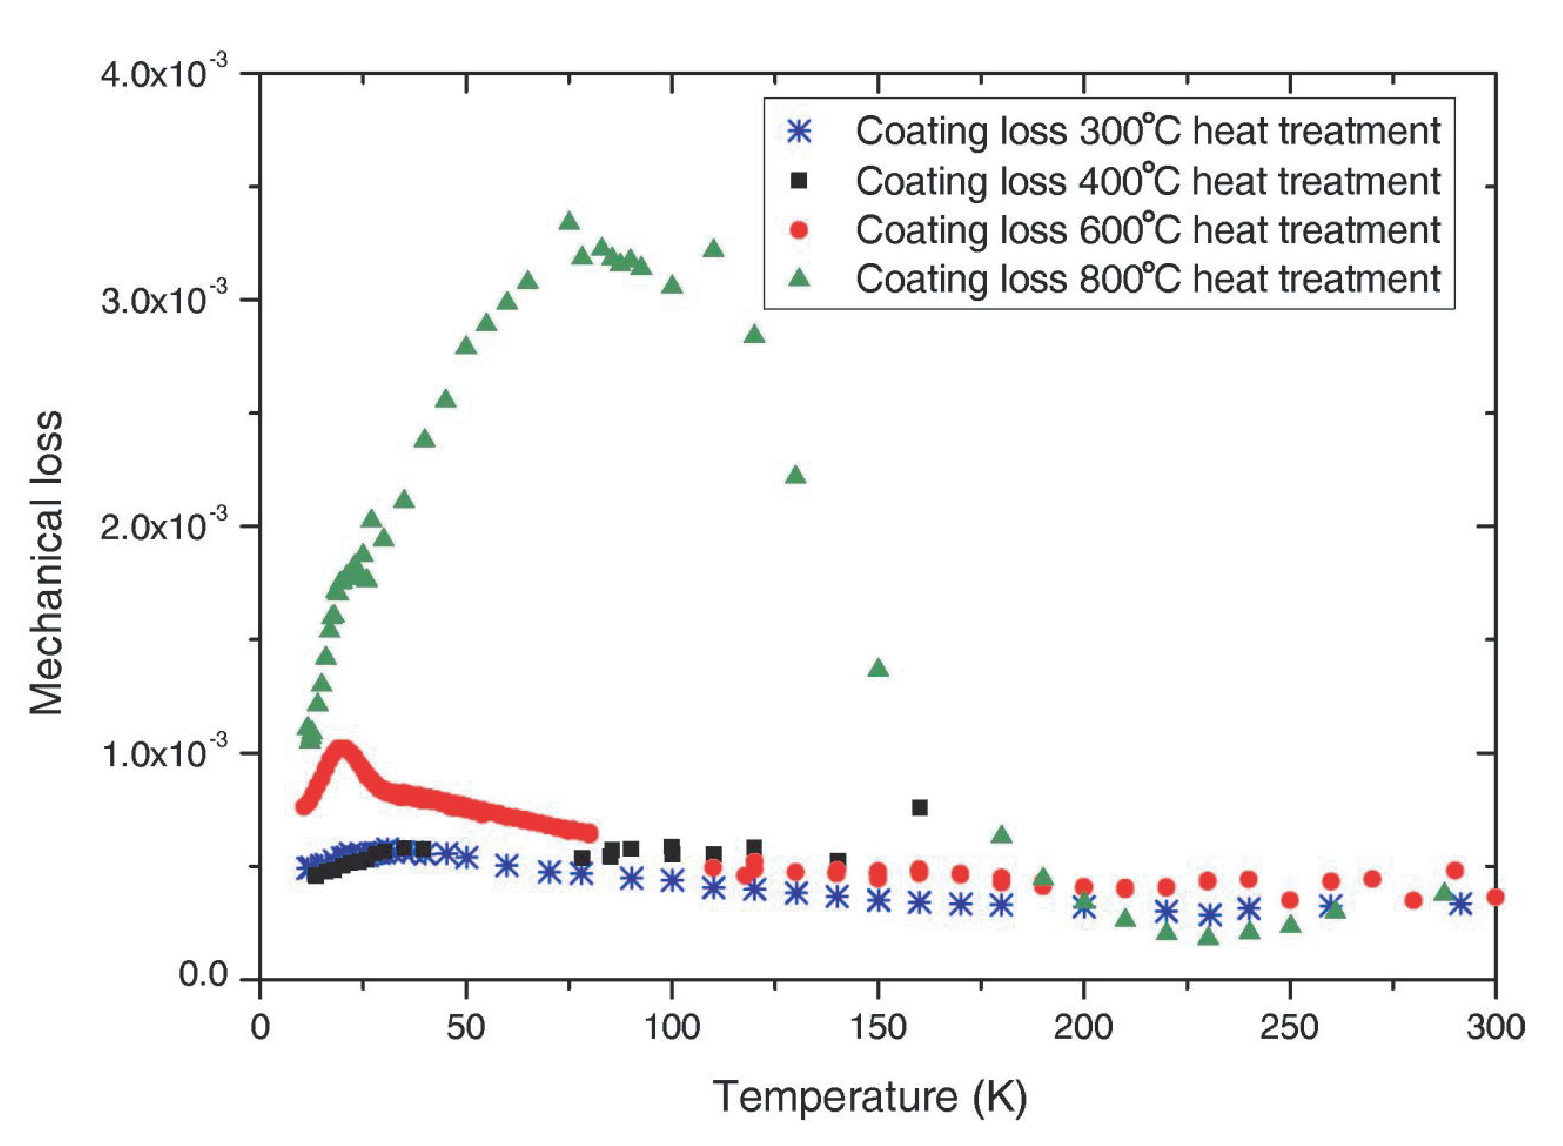
\includegraphics[width=0.49\linewidth]{Sec_Optics/coat_anneal.pdf}}
\subfigure[]{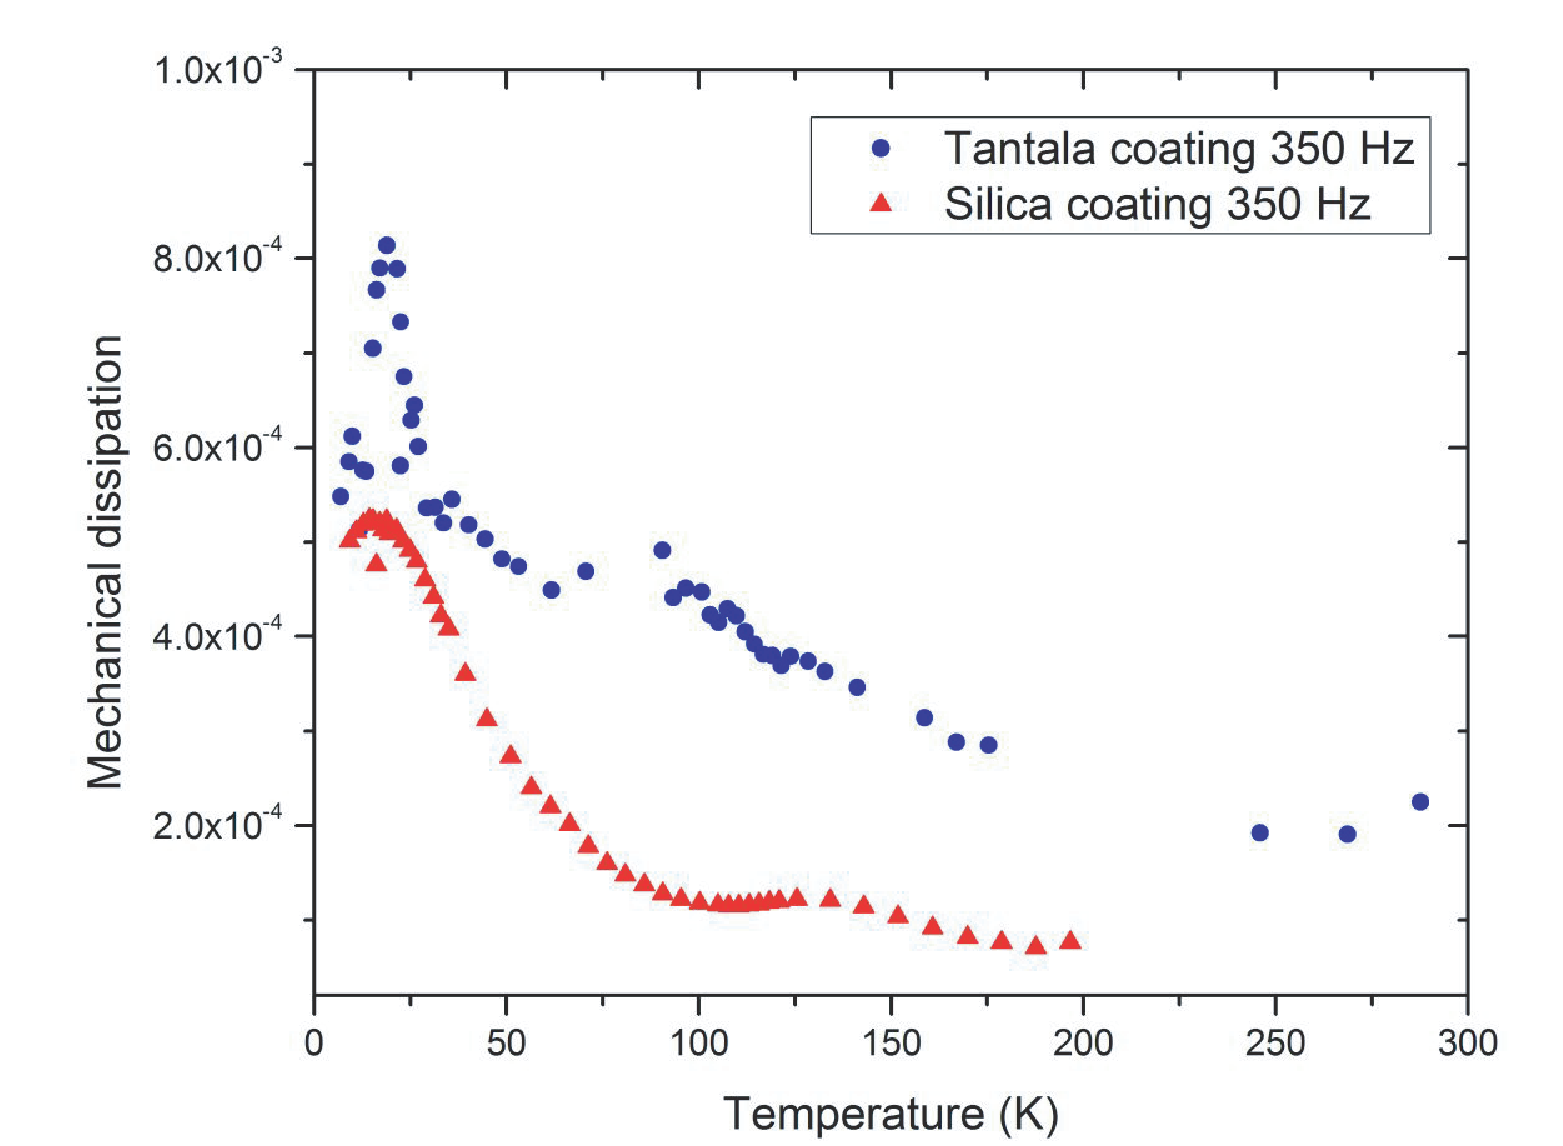
\includegraphics[width=0.49\linewidth]{Sec_Optics/silica_tantala_loss.pdf}}
\end{center}
\caption{(a)~--~Measured values of the coating loss of tantala annealed at different temperatures. (b)~--~Comparison of 600$\mathrm{^\circ}$C heat treated tantala and silica coatings at low temperatures and 350\,Hz.}
\label{fig:coating_loss_cryo}
\end{figure}

Further work may be required to establish the optimum heat-treatment temperature for a silica/tantala multilayer coating for use at cryogenic temperature. High heat-treatment temperatures are generally desirable for optimal optical properties. Furthermore, studies of the mechanical loss of ion-beam sputtered silica coatings have shown a systematic reduction in the loss at room temperature with increasing heat-treatment temperatures. Thus carrying out heat-treatment at the maximum temperature which can be achieved without inducing crystallisation in the tantala layers may be desirable. However, as shown in Figure~\ref{fig:coating_loss_cryo}(a), tantala has a significantly lower loss at temperatures below 100\,K when heat-treated at lower temperatures (300 or 400$\mathrm{^\circ}$C) than when heat-treated at 600$\mathrm{^\circ}$C. While the loss of the tantala layers dominate the loss of a multilayer silica/tantala coating at room temperature, the loss of ion-beam sputtered silica has a similar magnitude as the loss of tantala at temperatures below 50\,K. Thus further studies of the effect of heat-treatment on the temperature dependence of the mechanical loss of ion-beam sputtered silica are also required to allow the optimal heat-treatment temperature to be chosen. In addition, measurements of the temperature dependence of the optical properties of the coating may be required.

A comprehensive summary of R\&D activites needed for understanding and characterising the coating properties can be found in section~\ref{sec:coating_RND}.

\FloatBarrier
\subsubsection{Thermal noise estimates for reflective components}
\label{sec:TN_refl}

%\emph{Author: R. Nawrodt}

The thermal noise of a fully reflective mirror comprises thermal noise arising from the bulk material and the coating. The bulk material thermal noise consists of Brownian thermal noise and thermo-elastic noise. Brownian noise represents the thermal fluctuations (`Brownian motion') of the atoms within the bulk material and is dependent on the sample temperature $T$ and the mechanical loss of the bulk material $\phi$ \cite{Harry2002,Harry2006}:

\begin{equation}
S_\mathrm{x}^\mathrm{bulk}(f,T) = 2k_\mathrm{B}T\frac{1-\nu}{\pi^{3/2}fYw}\phi
\label{eq:bulk_Brownian}
\end{equation} 

with the Boltzmann constant $k_\mathrm{B}$, the frequency $f$, the beam radius $w$, the substrate Poisson's ratio $\nu$ and Young's modulus $Y$. It is obvious that the Brownian thermal noise is only dependent on mechanical properties of the material.

\longetbox{i}{box:TN}{Thermal noise in optical components}{There are two fundamental origins of thermal noise in optical components: The first is driven by the thermal energy $k_\mathrm{B}T$ that is present as soon as the component is operated at non-zero temperatures. Here, the thermal energy causes thermal fluctuations of the atoms of the optical component, which causes a thermally driven fluctuation of the reflective surface of the element. This type of noise is probably closest to the process that to mind when talking about thermal noise. In many different field this type of noise---Brownian noise---is present. Throughout this document this type of noise is called Brownian thermal noise.\\
However, there is a second type of noise that arises from temperature fluctuations. When operating a macroscopic object at non-zero temperatures the local (microscopic) temperature is not a constant value but fluctuates around the average temperature~$T$. Due to the fact that many material properties are temperature dependent this opens a channel to introduce the second type of noise. Here, the temperature fluctuation causes a phase or position fluctuation by means of the temperature dependence of a property, e.g.\ the coefficient of thermal expansion~$\alpha$ or the refractive index~$n$. The process that is associated with $\alpha$ is called thermo-elastic noise whereas the other process is referred to as thermo-refractive noise.\\
Although in both cases the temperature is the fundamental driving force one distinguishes between then strictly due to the different coupling mechanisms of the fluctuation to the read-out noise.}

The thermo-elastic noise of the bulk material is created by statistical temperature fluctuations. By means of the coefficient of thermal expansion $\alpha$ these fluctuations are translated into displacement noise. The thermo-elastic spectral noise density is given by~\cite{Braginsky1999a}:

\begin{equation}
S_\mathrm{TE}^\mathrm{bulk}(f,T) = \frac{4k_\mathrm{B}T^2\alpha^2(1+\nu)^2\kappa}{\sqrt{\pi^5}\rho^2C^2f^2w^3}
\label{eq:bulk_TE}
\end{equation}

with the coefficient of thermal expansion $\alpha$, the thermal conductivity $\kappa$, the heat capacity $C$, and the mass density $\rho$. This equation is valid if the thermal diffusion length 

\begin{equation}
l_\mathrm{th} = \sqrt{\frac{a^2}{f}}
\end{equation}

of the material is smaller than the beam diameter. The parameter $a^2 = \kappa/(\rho C)$. This assumption is called the adiabatic case. During one period of oscillation all temperature fluctuations that are present at the observation volume stay inside this volume. If the thermal diffusion length gets larger (e.g.\ by means of high thermal conductivity or low frequencies) the thermo-elastic effect gets weaker. Especially, for low temperature applications this non-adiabatic correction becomes important and reduces the contribution of thermo-elastic noise further. This correction has been taken into account for all calculations presented in this document. Details of the calculation can be found in~\cite{Cerdonio2001,Nawrodt2009_ET}.

Figure~\ref{fig:bulk_TN} compares the Brownian and thermo-elastic noise of one single mirror made of fused silica, sapphire or silicon at 10 and 300\,K. The parameters used for the calculation are listed in tables~\ref{tab:tn_T_param} and \ref{tab:tn_param}.

\begin{figure}
\begin{center}
\subfigure[]{\includegraphics[width=0.49\linewidth]{Sec_Optics/bulk_TN_300K.pdf}}
\subfigure[]{\includegraphics[width=0.49\linewidth]{Sec_Optics/bulk_TN_10K.pdf}}
\end{center}
\caption{Comparison of the Brownian and thermo-elastic noise for fused silica, sapphire and silicon at 300\,K~(a) and 10\,K~(b) (TE~--~thermo-elastic noise, FS~--~fused silica). At room temperature the crystalline substrate materials show a large thermo-elastic noise. In contrast, at cryogenic temperatures fused silica has a large Brownian thermal noise due to its large mechanical loss.}
\label{fig:bulk_TN}
\end{figure}

At room temperature fused silica provides the lowest level of thermal noise due to its low mechanical loss and small coefficient of thermal expansion (see figure~\ref{fig:bulk_TN}(a)). All crystalline materials show a high coefficient of thermal expansion and thus a large thermo-elastic noise. Therefore, crystalline materials should be avoided in room temperature detectors in order to achieve the minimum thermal noise level of a mirror substrate.

In contrast, at low temperatures fused silica has a large mechanical loss reaching values of $10^{-3}$ around 10\,K. Crystalline materials behave differently resulting in a low mechanical loss of better than $10^{-8}$ at low temperatures (see Tab.~\ref{tab:tn_T_param}). Additionally, the coefficient of thermal expansion is very small at low temperatures. This reduces dramatically the thermo-elastic noise contribution compared to room temperature operation (see figure~\ref{fig:bulk_TN}(b)). Thus, using cryogenic temperatures and crystalline materials will result in a low total bulk thermal noise.

\begin{figure}[!h]
\begin{center}
\subfigure[]{\includegraphics[width=0.49\linewidth]{Sec_Optics/bulk_Si_comp.pdf}}
\subfigure[]{\includegraphics[width=0.49\linewidth]{Sec_Optics/bulk_Sapphire_comp.pdf}}
\end{center}
\caption{Comparison of the total bulk thermal noise of a mirror substrate made of silicon~(a) and sapphire~(b) at different temperatures. The parameters used for this calculation are summarised in tables~\ref{tab:tn_T_param} and \ref{tab:tn_param}.}
\label{fig:bulk_T_TN}
\end{figure}

Figure~\ref{fig:bulk_T_TN} compares the total bulk thermal-noise consisting of thermo-elastic and Brownian thermal noise for sapphire and silicon at selected temperatures. Due to the small mechanical loss and coefficient of thermal expansion, a low thermal noise level is achieved. At 20\,K both materials show a comparable thermal noise level. At higher temperatures thermo-elastic noise becomes dominant. Here, sapphire has a slightly lower level of thermo-elastic noise due to the combination of its thermal properties (mainly the high thermal conductivity). At 10\,K silicon has a slightly lower total thermal noise than a sapphire mirror substrate. 

All calculations so far are based on semi-infinite mirror substrates. This assumption is true for a first comparison of the materials and in cases where the beam radius compared to the mirror radius is small. However, for application in gravitational wave detectors it is preferable to increase the beam diameter to the maximum possible size that is in agreement with the optical clipping losses. The corrections for finite size test masses have been made by different authors for the different noise contributions. The calculations are quite long and thus only the results are shown here. The detailed discussion can be found in the literature \cite{Bondu1998, Liu2000}. 

\begin{figure}[!h]
\begin{center}
\subfigure[]{\includegraphics[width=0.49\linewidth]{Sec_Optics/bulk_FTM_thick.pdf}}
\subfigure[]{\includegraphics[width=0.49\linewidth]{Sec_Optics/bulk_FTM.pdf}}
\end{center}
\caption{Finite size test mass mirror thermal noise. (a)~--~Dependence of the mirror Brownian and thermo-elastic thermal noise of the thickness of the substrate (silicon, 10\,K, diameter: 0.5\,m, frequency 10\,Hz). (b)~--~Effect of the finite size correction for a typical ET end mirror geometry (silicon, 10\,K). BB~--~bulk Brownian, TE~--~thermo-elastic, ITM~--~inner test mass, ETM~--~end test mass.}
\label{fig:bulk_TN_finite}
\end{figure}

Figure~\ref{fig:bulk_TN_finite} gives the dependence of the substrate thermal noise. It is obvious that for reasonable thicknesses of the substrate the correction is small. Only for very thin substrates does a strong deviation from the simplified infinite half space model appear. At larger thicknesses the finite sample correction leads to a small decrease in thermal noise (approx. $5\dots 10\%$ for bulk Brownian and less than 1\% for bulk thermo-elastic noise).

Optical components being used in GW detectors consist of a bulk material and a coating. The coating usually comprises several alternating dielectric layers formed by high and low refractive index materials. Typically, these layers are formed by amorphous tantala and silica layers with an optical thickness of $\lambda/4$. The circulating laser beam of the interferometer interacts mainly with the coating (point of first contact between light and mirrors). Thus, it can be expected that the optical coating contributes strongly to the total thermal noise of a mirror.

Similar to the thermal noise of the bulk materials, the coatings also show Brownian thermal noise. It is again dependent on the temperature $T$ and the effective mechanical loss $\phi_\mathrm{eff}$ of the coating \cite{Harry2002,Harry2006}:

\begin{equation}
S_x^\mathrm{coating}(f,T) = 2k_\mathrm{B}T\frac{1-\nu}{\pi^{3/2}fYw}\phi_\mathrm{eff}
\label{eq:coat_Brownian}
\end{equation}

with the Boltzmann constant $k_\mathrm{B}$, the frequency $f$, the beam radius $w$, the Poisson's ratio $\nu$ and the Young's modulus $Y$ of the substrate bulk material. The effective mechanical loss contains all coating relevant parameters and is given by:

\begin{equation}
\phi_\mathrm{eff} = \frac{t}{\sqrt{\pi}w}\left(\frac{Y}{Y_\bot}\phi_\bot + \frac{Y_{||}}{Y}\phi_{||} \right).
\label{eq:coat_eff_loss}
\end{equation}

This description of the effective mechanical loss assumes small Poisson's ratios of the coating materials, which is usually fulfilled. $t$ is the total thickness of the coating layer. The Young's moduli $Y_i$, the thicknesses $t_i$ and the mechanical losses $\phi_i$ are combined as follows ($i=1,2$ to indicate the different coating layer properties):

\begin{eqnarray}
Y_\bot & = & \frac{t_1+t_2}{\frac{t_1}{Y_1}+\frac{t_2}{Y_2}}, \\
Y_{||} & = & \frac{Y_1t_1 + Y_2t_2}{t_1+t_2}, \\ 
\phi_\bot & = & \frac{Y_\bot}{t_1+t_2} \left(\frac{t_1}{Y_1}\phi_1+\frac{t_2}{Y_2}\phi_2 \right) \\
\phi_{||} & = & \frac{Y_1t_1\phi_1 + Y_2t_2\phi_2}{Y_{||}\left(t_1+t_2\right)}
\label{eq:coat_aniso_param}
\end{eqnarray}

Light penetrates the first  dielectric layers of a high-reflective mirror and thus interacts not only with the front surface. Here, a fluctuating local temperature causes a change in the thickness of the layer by means of the coefficient of thermal expansion $\alpha$ and additionally a change of the refractive index $n$ of the materials. In total, these two effects sum up and change the optical path of the light being reflected. This statistical process combining effects of thermo-elastic (due to $\alpha$) and thermo-refractive (due to the change of $n$) is called thermo-optical noise. Depending on the sign of $\alpha$ and $dn/dT$ these two effects can result in a smaller noise than the two terms predict separately.

Thermo-optical noise can be calculated following the approach by Evans et al. in 2008. The calculation is too complex to be presented here---see \cite{Evans2008} for the full description of it. 

\begin{figure}[!h]
\begin{center}
\subfigure[]{\includegraphics[width=0.49\linewidth]{Sec_Optics/coating_low_TN.pdf}}
\subfigure[]{\includegraphics[width=0.49\linewidth]{Sec_Optics/coating_low_TN_TO.pdf}}
\end{center}
\caption{(a)~--~Comparison of coating Brownian noise at different temperatures. (b)~--~Comparison of coating thermo-optical and Brownian noise at room temperature. Both calculations assume a 18 doublet alternating silica-tantala quarter wavelength layer with a $\lambda/2$-endcap. The coating is assumed to be put on a silicon substrate. A wavelength of 1550\,nm was used for the estimates.}
\label{fig:coat_TN}
\end{figure}


Figure~\ref{fig:coat_TN} compares the Brownian and thermo-optical noise levels of different coatings at low temperatures and room temperature. Parameters are used from tables~\ref{tab:summary14}, \ref{tab:tn_T_param}, \ref{tab:tn_param} and \ref{tab:Coat_param}. A direct comparison at 10\,K reveals that the thermo-optical noise is much smaller than the coating Brownian noise. This statement is also true for higher temperatures which makes thermo-optical noise not a dominating source of total thermal noise of a reflective component for a gravitational wave detector.

\longetbox{h}{box:optemp}{Operational Temperature of ET-LF}{The design temperature of the low frequency interferometer of ET was chosen to be 10\,K. This value arises directly from different restrictions. From a thermal noise point of view the lowest possible temperature would be desirable. However, this collides with the necessary heat removal through the suspension as given in section \ref{sec:mat_lss}. At very low temperatures (well below 10\,K) the thermal conductivity of the suspension materials will be very low and it is impossible to remove the deposit heat from the laser beam through the fibres. The maximum tolerable temperature from a point of view of thermal noise is around 24\,K (see Fig.\,\ref{fig:tn_etlf2}). However, as can be seen from Fig.~\ref{fig:coating_loss_cryo} the currently proposed coating material tantala shows a large loss peak around 18\,K when it is annealed to 600 degrees to improve the optical quality. Thus the final decision has been made to go as low as possible in operational temperature to stay below that dissipation peak that would cause an increased level of coating Brownian noise. A summary of the total mirror thermal noise at different temperatures can be found in the appendix \ref{sec:tn_etlf}.}

The level of coating Brownian noise is additionally larger than the total noise level of the bulk material presented in figure~\ref{fig:bulk_T_TN}. Thus, coating Brownian noise is the most important type of thermal noise of a high reflective mirror and great care must be taken in choosing the optimum operational temperature and the appropriate material combination. Avoiding the mechanical loss peak in amorphous dielectric coatings at around 15 to 30\,K (depending on the actual material, see figure~\ref{fig:coating_loss_cryo}) was one of the strongest reasons for the 10\,K target temperature of the cooled mirrors of the ET-LF detector.

Details of the ongoing and future research in the field of mechanical losses of bulk and coating materials as well as other thermal noise issues are given in section~\ref{sec:RD}.


\FloatBarrier
\subsubsection{Thermal noise estimates for transmittive components}
\label{sec:TN_trans}
%\emph{J. Franc}

The total thermal noise of a transmittive component considers the noise contribution described in the previous subsection and additionally the thermo-refractive noise that occurs from statistical fluctuations of the refractive index $n$ due to its temperature dependence $dn/dT$. A temperature fluctuation produces a small change of $n$ which leads to phase changes detected by the interferometer. The thermo-refractive noise has been calculated by equations given by Braginsky~\cite{Braginsky2004} in addition with correction terms developed by Benthem and Levin~\cite{Benthem2009}.

Taking into account the configuration of Einstein Telescope given in figure~\ref{Fig:opt_lay_over} and table~\ref{tab:summary14} results in the following equation for the thermo-refractive noise (power spectral density) in an interferometer with arm cavities of finesse~$F$:

\begin{align}
S_h(f,T)&=\frac{4}{L^2}\left(\frac{\lambda}{8F}\right)^2 \nonumber \\
&\left(kl \beta\right)^{2} \frac{4k_B T^{2} \kappa}{\left(C\rho\right)^{2}l}
\left(1+\frac{\left(kn\right)^{2}w^{2}}{\left(1+\left(2kn\sqrt{\frac{\kappa}{C
\rho\omega}}\right)^{4}\right)}\right) \int_0^{\infty}{\frac{k_i dk_i}{2\pi} \exp \left(\frac{-w^2k_{i}^{2}}{4}\right) \frac{k_{i}^2}{\omega^2+a^4 k^4 }}, 
\label{eq:Tref}
\end{align}

where
\begin{equation}
k=\frac{2 \pi}{\lambda}
\label{eq:k}
\end{equation}

and 

\begin{equation}
{a}^2=\frac{\kappa}{C\rho}.
\end{equation}

$l$ is the thickness of the input mirror, $\beta$ the thermo-optic coefficient of the substrate material, $T$ is the temperature, $k_B$ the Boltzmanns constant, $\kappa$ the thermal conductivity, $C$ the specific heat, $\rho$ the density of the substrate material, $w$ is the beam radius, $L$ the arm length of the interferometer, and $n$ the refractive index of the substrate material. Details of this equation can be found in~\cite{Franc2010}.

At 300\,K the silica substrate provides the lowest thermo-refractive noise (see figure~\ref{fig:Bulk_Tref_300K}). Substrate materials with a low thermo-optic coefficient show a low thermo-refractive noise. As a numerical result, for silica, sapphire and silicon, it is respectively $8\times10^{-6}$, $1.3\times10^{-5}$ and $5.15\times10^{-5}$. 

\begin{figure}[!h]
\begin{center}
\includegraphics[width=0.49\linewidth]{Sec_Optics/Bulk_Tref_comp_300K.pdf}
\caption{Substrate thermo-refractive noises for silica, sapphire and silicon at room temperature.}
\label{fig:Bulk_Tref_300K}
\end{center}
\end{figure}

Then, the thermo-refractive noise is compared for silicon and sapphire as the most promising test mass materials at cryogenic temperatures. The substrate thermo-refractive noise is largely dependent on the thermo-optic coefficient. This value has been measured for sapphire at low temperatures and reaches $9\times 10^{-8}\,\mathrm{K}^{-1}$ below 4\,K~\cite{Tomaru2002a}. For silicon the parameter is not very well known. The only currently literature source available reports values of $n$ and $dn/dT$ down to 30\,K~\cite{Frey2006}. However, the values reported for $dn/dT$ do not agree with the slope of the $n(T)$ curve of the same reference. Thus, the knowledge of the parameter is strongly limited. At temperatures around 20\,K a value of $1\times10^{-6}\,\mathrm{K}^{-1}$ can be assumed as an upper limit of $dn/dT$ based on the experimental values given in~\cite{Frey2006}. At even lower temperatures it is reasonable to assume a further decrease of the value due to thermodynamical assumptions: at 0\,K all temperature dependent properties have to become constant---thus the temperature derivative has to vanish.

Figure~\ref{fig:Tref_a} shows the thermo-refractive noise of silicon and sapphire at 10\,K based on equation~(\ref{eq:Tref}) given above. The $dn/dT$ for silicon is assumed as $1\times10^{-6}\,\mathrm{K}^{-1}$ and the $dn/dT$ for sapphire is $9\times10^{-8}\,\mathrm{K}^{-1}$.

\begin{figure}[!h]
\begin{center}
\subfigure[]{\includegraphics[width=0.49\linewidth]{Sec_Optics/Comp_SiandSa.pdf}\label{fig:Tref_a}}
\subfigure[]{\includegraphics[width=0.49\linewidth]{Sec_Optics/Comp_Temp_TRef.pdf}\label{fig:Tref_b}}
\caption{(a)~--~Substrate thermo-refractive noise of silicon and sapphire at 10\,K (beam size: 9\,cm). (b)~--~Substrate thermo-refractive noise of silicon at 10\,K, 20\,K, 30\,K ($dn/dT$ unchanged:\ $1\times10^{-6}\,\mathrm{K}^{-1}$).}
\end{center}
\end{figure}

Sapphire shows a very small thermo-refractive noise due to its small thermo-refractive coefficient $\beta$. Although it is higher, the thermo-refractive noise of a silicon substrate is also very low and should not affect the total thermal noise of the system. The operational frequency of the LF detector is between 1 and 250\,Hz. Above this frequency the HF detector takes over and limits the sensitivity of the Einstein Telescope. It is expected that experimental values for the thermo-refractive coefficient of silicon is even lower than the one given here (see section~\ref{sec:RD}).

Figure~\ref{fig:Tref_b} shows the evolution of the thermo-refractive noise for different temperatures (10\,K, 20\,K, 30\,K). It shows that the thermo-refractive noise decreases with the temperature. Thus, operating at the highest possible temperature that allows a low thermal noise operation is preferred. This leads to a possible optimization process.

\FloatBarrier
\subsubsection{LF interferometer large mirror definition}
%\emph{Author(s): J. Franc}\\ 
\label{sec:LF_mirror_def}

The Einstein Telescope detector is split into two interferometers (ET-LF and ET-HF) due to thermal noise and heating reasons. The ET-LF detector assumes a beam radius size of 9\,cm, corresponding to an effective test mass diameter of 45-50\,cm, but at the same time keeps the overall test mass weight at about 210\,kg~\cite{Hild2010b} with sufficient thickness.
This mass leads to a thickness for a future silicon test mass of approximately 46-50\,cm. The thickness would drop to about 30\,cm for sapphire due to the higher material density. For the substrate, the thermo-refractive noise is dependent on the thickness of the mirror. 

\begin{figure}[!h]
\begin{center}
\includegraphics[width=0.49\linewidth]{Sec_Optics/LFSiandSa.pdf}
\caption{Substrate thermo-refractive noise of silicon ($w=9$\,cm, thickness~50\,cm) and sapphire ($w=9$\,cm, thickness~50\,cm) substrate compared to the ET-D sensitivity.}
\label{fig:LFSiandSa}
\end{center}
\end{figure}

Figure~\ref{fig:LFSiandSa} shows that the thermo-refractive noise of silicon and sapphire is well below the ET sensitivity target. Therefore, we can foresee that the assumed dimensions are possible and promising. A plot of all the thermal noises for silicon and sapphire is shown in Figure~\ref{fig:SiandSa}. 

\begin{figure}[!h]
\begin{center}
\subfigure[]{\includegraphics[width=0.49\linewidth]{Sec_Optics/Simirror.pdf}}
\subfigure[]{\includegraphics[width=0.49\linewidth]{Sec_Optics/Samirror.pdf}}
\caption{(a)~--~Thermal noise contribution for a silicon mirror ($w=9$\,cm, thickness 50\,cm, $T=10$\,K). (b)~--~Thermal noise contribution for a sapphire mirror ($w=9$\,cm, thickness 30\,cm, $T=10$\,K).}
\label{fig:SiandSa}
\end{center}
\end{figure}

For a silicon mirror, thermal noise is dominated by the coating Brownian noise and the substrate thermo-refractive noise. Coating Brownian noise is, in reality, higher than all other noises considered but still below the ET-LF sensitivity target. For a sapphire substrate, coating Brownian noise is also the highest thermal noise. Therefore, a cooled silicon (or sapphire) mirror provides a low enough thermo-refractive noise in the frequency band covered by the LF detector. 

In conclusion, both materials---sapphire and silicon---provide low thermo-refractive noise levels that are compatible with the requirements for the Einstein Telescope. An exact estimate of the thermo-refractive noise level of silicon will not be possible until the thermo-refractive coefficient is measured for different types of silicon. It can be expected that this parameter strongly depends on the level of doping. Several institutions are currently working on experiments to extend the existing parameters to temperatures below 30\,K.


%\emph{Author(s): R. Nawrodt} \\

Based on the calculations presented in sections~\ref{sec:TN_refl} and \ref{sec:TN_trans} it is now possible to give an overall estimate of the expected thermal noise from the optical components of the ET-LF detector. The total estimate is based on the simplified sketch of the ET-LF detector in figure~\ref{Fig:opt_lay_over}. The input coupler of the cavity as well as the end test mass are cooled to cryogenic temperatures around 10\,K. The beam splitter is operated at room temperature. 

In order to achieve a good thermal noise performance of the optical components a large beam radius $w$ as large as 90\,mm is needed. This requires the use of large diameter bulk samples to avoid large clipping losses. This requirement lead to a typical substrate diameter of 50\,cm. In addition the suppression of radiation pressure noise requires large masses---for the ET-D design a mass of 211\,kg is needed. In combination with the maximum available diameter of a potential silicon test mass material this leads to a required minimum thickness of 46\,cm for the optical components involved in the arm cavities (end test mass and input coupler). A further increase of the thickness will reduce radiation pressure noise further---however, it will increase the thermo-refractive noise of the input test mass. 

The option to use sapphire as a test mass material seems to be strongly limited by the availability of the materials. So far, it is not expected that by the time ET will be built sapphire test masses with a required diameter of 50\,cm will be available on the market. Thus, all estimates in this section are based on the choice of silicon as a test mass material---although sapphire will totally satisfy all noise demands if operated at the same temperature and if it is available in the same geometry.

Figure~\ref{fig:ET_LF_ETM_total} shows the total thermal noise of an end test mass cavity mirror for ET. The calculations are based on the properties presented in tables~\ref{tab:summary14}, \ref{tab:tn_T_param}, \ref{tab:tn_param}, and \ref{tab:Coat_param}. A silicon test mass with a diameter of 50\,cm and a thickness of 46\,cm was assumed to be operated at 10\,K. The ETM uses 18 $\mathrm{\lambda/4}$-doublets of tantala/silica layers and the ITM 9 $\mathrm{\lambda/4}$-doublets of tantala/silica to form the cavity. While the laser beam reads out the surfaces of the cavity mirrors 

\begin{equation}
N=2/\pi F
\label{eq:red_factor}
\end{equation}

times ($F$~--~finesse of the cavity) it only senses the thermo-refractive noise of the ITM twice (input and output of the cavity). This reduction factor is included for the ITM and the thermo-refractive noise recalculated as an effective displacement noise for comparison.

\begin{figure}[!h]
\begin{center}
\subfigure[\label{fig:ET_LF_ETM_total}]{\includegraphics[width=0.49\linewidth]{Sec_Optics/ET_LF_ETM_TN.pdf}}
\subfigure[\label{fig:ET_LF_ITM_total}]{\includegraphics[width=0.49\linewidth]{Sec_Optics/ET_LF_ITM_TN.pdf}}
\end{center}
\caption{Total thermal noise of an end test mass~(a) and an input test mass~(b) of the arm cavity of ET-LF. Both substrates are assumed to be made of silicon with a diameter of 50\,cm and a thickness of 46\,cm. The operational temperature is 10\,K. The ETM is equipped with 18 $\mathrm{\lambda/4}$-doublets of a tantala/silica high-reflective stack while the ITM is coated with 9 $\mathrm{\lambda/4}$-doublets to achieve a transmission of about 7000\,ppm.}
\end{figure}

For both---the ETM and the ITM---the coating Brownian noise dominates over all frequencies. For the input test mass the required 46\,cm thickness leads already to significant contributions from the thermo-refractive noise. The uncorrelated sum of the different noise contributions in the ETM and the ITM can be used as a good estimate for the total thermal noise contribution of one arm cavity. 

An additional noise source in the interferometer is the beam-splitter. Due to the fact that this element is situated outside the arm cavities its thermal noise contribution to the overall thermal noise of the detector is again reduced by the factor given in eq.~(\ref{eq:red_factor}). Thus, cooling might not be needed for this component. The beam splitter is assumed to be made of fused silica and operated at room temperature. The different thermal noise contributions based on the equations given in the previous sections are summarised in figure~\ref{fig:ET_LF_BS_TN}. The beam splitter is assumed to be coated with 3 $\mathrm{\lambda/4}$-doublets of tantala/silica as an upper limit calculation. The thickness of the beam splitter is 10\,cm and the aspect ratio is kept similar to the end test masses. 

\begin{figure}[!h]
\begin{center}
\subfigure[\label{fig:ET_LF_BS_TN}]{\includegraphics[width=0.49\linewidth]{Sec_Optics/ET_LF_BS_TN.pdf}}
\subfigure[\label{fig:ET_LF_BS_total}]{\includegraphics[width=0.49\linewidth]{Sec_Optics/ET_LF_BS_total.pdf}}
\end{center}
\caption{(a)~--~Summary of the different thermal noise sources in a potential ET-LF beam splitter made of fused silica and operated at room temperature. (b)~--~Evolution of the total thermal noise of the beam splitter with different beam radii at the beam splitter.}
\end{figure}

The thermo-refractive contribution from the beam-splitter is based on the calculation by Benthem and Levin for GEO600~\cite{Benthem2009}. Thermo-refractive noise is the most dominating noise source of the beam splitter due to the very low mechanical loss of fused silica at room temperature and the small number of coating layers. If the beam radius of the laser beam at the beam splitter is further reduced, thermo-refractive noise increases as shown in fig.~\ref{fig:ET_LF_BS_total}. This reduction of the beam radius might be beneficial to reduce the necessary size of the beam splitter. Due to the fact that the beam splitter is operated under an angle the necessary size is increased compared to an end mirror. These mirrors are currently already designed to be at or close to the edge of what is and will be available by the time ET will be built. Thus, a reduction of the dimensions of the beam splitter is needed. 
 
Combining all noise contributions from the two arm cavities and the beam splitter (incoherent sum) leads to an estimate of the total thermal noise contribution for ET-LF, which is given in figure~\ref{fig:ET_LF_total_TN} for different beam radii at the beam splitter.

\begin{figure}[!h]
\begin{center}
\includegraphics[scale=0.7]{Sec_Optics/ET_LF_noise.pdf}
\end{center}
\caption{Total thermal noise arising from the optical components of ET-LF for different beam radii at the beam splitter.}
\label{fig:ET_LF_total_TN}
\end{figure}

It is obvious that the main thermal noise contribution comes from the arm cavities. Even if the beam radius at the beam splitter is chosen to be as small as 0.5\,cm the noise contribution from the beam splitter is smaller than the contribution from the arm cavities. This relaxes the demands for the size of the beam splitter and the thermal noise contribution of the beam splitter is in agreement with the proposed beam diameter at the beam splitter of 6\,mm.

\FloatBarrier
\subsubsection{HF interferometer large mirror definition}
%\emph{Author(s): J. Franc \\}

Fused silica is the material of choice for the high frequency detector operating at room temperature. Fused silica is one of the most commonly used materials in optics and has been improved during many decades. Appropriate polishing methods exist to obtain a very high surface quality. Fused silica has remarkable properties at room temperature: low mechanical loss (see section~\ref{app:mechdat}) which leads to a small substrate Brownian noise, and an exceptional low coefficient of thermal expansion (see section~\ref{app:thermdat}) which results in a small thermo-elastic noise.

\begin{table}[!h]
\begin{center}
\begin{tabular}{|c|c|} \hline
Parameter & ET-HF \\ \hline
temperature & 290\,K \\
arm length & 10\,km \\ 
mirror material & Fused silica \\
mirror diameter & 62\,cm \\
mirror thickness & 30\,cm \\
mirror mass & 200\,kg \\
laser wavelength & 1064\,nm \\
beam shape & TEM$_{00}$ \\
beam radius & 12\,cm \\
coating high index & $\mathrm{Ti:Ta_2O_5}$ \\
coating low index & $\mathrm{SiO_2}$ \\ 
\hline
\end{tabular}
\end{center}
\caption{Summary of the parameters used for the thermal noise estimate of the HF interferometer.}
\label{tab:HF_dat}
\end{table}

The assumed parameters for the ET-HF interferometer are listed in Table~\ref{tab:HF_dat}. The mirror geometry was chosen so that the mass reaches 200\,kg to suppress radiation pressure noise and that the mirror geometry causes only 1\,ppm diffraction loss at its boundaries~\cite{Vinet2007}. For the sake of simplicity, in this estimates a TEM$_{00}$ beam has been taken into account, considering the use of LG$_{33}$ as an option for the HF interferometer. Using LG$_{33}$ modes will further reduce thermal noise. However, it will be shown that the currently assumed geometry is already compliant with the ET-HF sensitivity curve if a TEM$_{00}$ mode is assumed.

In order to compare the behaviour of different substrate materials the thermal noise of a high reflectivity mirror was calculated using the same `standard' coating and different substrate materials. The `standard' coating is a multilayer $\mathrm{(HL)_{17}HLL}$ coating made of $\mathrm{Ti:Ta_2O_5}$ and $\mathrm{SiO_2}$ quarter wavelength layers. On a fused silica substrate this coating corresponds to a transmission of 6\,ppm. The lowest mechanical loss experimentally observed has been considered for the coating materials (see section~\ref{app:mechdat}). The result of this comparison is shown in Figure~\ref{fig:substrate_comp}. The graph plots different noise sources in the substrate materials as well as their coatings. 

\begin{figure}[!h]
\begin{center}
\includegraphics[width=0.49\linewidth]{Sec_Optics/substrate_comp.pdf}
\caption{Total thermal noise of three different substrates at 300\,K: silica, sapphire, and silicon at 1550\,nm. }
\label{fig:substrate_comp}
\end{center}
\end{figure}

At 300\,K, the total thermal noise for silicon is limited by two substrate thermal noises: substrate Brownian noise at high frequencies and substrate thermo-elastic noise at low frequencies. Sapphire must also be discarded due to its large thermo-elastic noise at low frequencies. Therefore, the most adapted substrate at room temperature is fused silica. In this case, coating limits the sensitivity of the future detectors only through its Brownian thermal noise. 

\paragraph{Mirror coating}
%\emph{Author(s): J. Franc} \\ 

As explained above, the total thermal noise of the test masses is a combination of coating Brownian, substrate Brownian, substrate thermo-elastic, substrate thermo-refractive, and thermo-optic noise. Taking into account these five noise sources, the coating Brownian noise is the most important one and can limit the sensitivity target. A state-of-the-art of different coating material have been realized in order to compare different combination of multilayer stacks.  

Figure~\ref{fig:coating} shows the total thermal noise for different coatings on a silica substrate at room temperature. The calculations are based on the currently best available data of the materials (table~\ref{tab:Coat_param}). Each coating corresponds to a transmission of 6\,ppm on a fused silica mirror. Therefore, all multilayers are different according to materials taken into account.

We need:

\begin{itemize}
	\item $\mathrm{(HL)_{17}HLL}$ for a coating made of $\mathrm{Ti:Ta_2O_5}$ and $\mathrm{SiO_2}$ quarter wavelength layers,
	\item $\mathrm{(HL)_{13}HLL}$ for a coating made of $\mathrm{TiO_2}$ and $\mathrm{SiO_2}$,
	\item $\mathrm{(HL)_{13}HLL}$ for a coating made of $\mathrm{Nb_2O_5}$ and $\mathrm{SiO_2}$,
	\item $\mathrm{(HL)_{16}HLL}$ for a coating made of $\mathrm{ZrO_2}$ and $\mathrm{SiO_2}$,
	\item $\mathrm{(HL)_{24}HLL}$ for a coating made of $\mathrm{Ti:Ta_2O_5}$ and $\mathrm{Al_2O_3}$, and
	\item $\mathrm{(HL)_{22}HLL}$ for a coating made of $\mathrm{ZrO_2}$ and $\mathrm{Al_2O_3}$.
\end{itemize}

According to the refractive index of the material the number of layers can vary by a factor of two. 

\begin{figure}[!h]
\begin{center}
\includegraphics[bb=100 270 500 570,width=0.49\linewidth]{Sec_Optics/coating.pdf}
\end{center}
\caption{Comparison of the thermal noise of different coating materials on a fused silica substrate at room temperature.}
\label{fig:coating}
\end{figure}

There is a clear advantage for the $\mathrm{SiO_2-Ti:Ta_2O_5}$ coating showing the lowest coating thermal noise.
The results obtained for $\mathrm{SiO_2-Nb_2O_5}$ and $\mathrm{SiO_2-ZrO_2}$ are encouraging as well. However, if we include the optical absorption of the coatings, the use of the standard coating is even more strongly supported. So far, there is no better coating to be used at room temperature than the $\mathrm{Ti:Ta_2O_5-SiO_2}$. 

\begin{figure} [!h]
\begin{center}
\includegraphics[bb=100 270 500 570,width=0.49\linewidth]{Sec_Optics/silicaTTN.pdf}
\end{center}
\caption{Contribution of the different thermal noises for a fused silica mirror at room temperature.}
\label{fig:silicaTTN}
\end{figure}

In conclusion, we have evaluated the total mirror thermal noise at room temperatures by implementing a model that includes Brownian, thermo-elastic and thermo-refractive noise. From the different calculations we have presented based on the parameters listed above we draw the conclusion that fused silica is the best test mass material for the high frequency detector of the 3rd generation GWD. The optimized mirror for the HF interferometer is, at present, a fused silica test mass with a diameter of 62\,cm and a thickness of 30\,cm.

%------
%\FloatBarrier
\subsubsection{Mirror surface defects}
\label{sec:msurface}

%\emph{Author(s): M. Galimberti, K. Kokeyama}\\ 

Here we discuss investigations of mirror surface defects in order to understand their effects on cavity resonance and losses, and to define requirements for surface polishing. For convenience, the mirror surface deviations from the perfect surface can be classified into two categories, depending on their spatial frequencies. Defects in the high frequency range (above a few hundred m$^{-1}$) will scatter light outside the cavity and thus generate cavity losses and scattering noise. Defects in the spatial low frequency range (between 1 and 100\,m$^{-1}$) may induce resonance of unwanted modes in the cavity, and thus degrade the mode purity inside the cavity.
 
 % from LMA presentations in Jena, Kyoto, and Budapest (2010)
The ET arm cavities were simulated by FFT propagation using the simulation software \emph{SIESTA}~\cite{Caron1999}. Artificial mirror maps were applied to both mirrors of the cavity. The artificial maps were randomly generated in order to reproduce a defect distribution similar to that found in actual VIRGO and LIGO mirrors~\cite{Galimberti2010a, Galimberti2010, Galimberti2010b}.  

Table~\ref{tab:msurface} shows the cavity gain and round-trip losses for the fundamental mode resonating in the cavity (wavelength of 1064 or 1550\,nm), with varying RMS flatness of the surface defects. The distribution of defects considered here goes as $f^{-2}$, where $f$ is the spatial frequency. It has been shown in~\cite{Galimberti2010b} that such a distribution, with a RMS of 1.0\,nm, overestimates the low-frequency defects with respect to what has already been obtained for the Advanced LIGO mirrors. Therefore the surfaces obtained by current polishing techniques seem already good enough to obtain reasonably small round-trip losses for the fundamental mode. Using a wavelength of 1550~nm is particularly favourable from this point of view (smaller losses).
 
\begin{table}[h]
\begin{center}
\begin{tabular}{ccccc}
%
\hline
RMS flatness 	& \multicolumn{2}{c}{TEM$_{00}$ 1064\,nm} 	& \multicolumn{2}{c}{TEM$_{00}$ 1550\,nm}\\
				& cavity gain 	& r.t.\ losses [ppm]			& cavity gain 	& r.t.\ losses [ppm]		\\
\hline
0\,nm 			& 567.4			& 2							& 567.4			& 3						\\
0.5\,nm			& $564.5\pm0.9$	& $20\pm6$					& $566.7\pm0.3$	& $7\pm2$				\\
1.0\,nm			& $555.9\pm3.7$	& $73\pm24$					& $564.4\pm0.9$	& $21\pm6$				\\
\hline
%
\end{tabular}
\end{center}
\caption[Round-trip losses as a function of surface defects]{Cavity gain and round-trip losses for the arm cavities, computed from FFT simulations, as a function of surface defects RMS. The fundamental TEM$_{00}$ mode is considered, for the wavelengths 1064 and 1550\,nm. Data are expressed as mean${}\pm{}$standard deviation on an ensemble of 10 different cavities. For each cavity, random surface maps with a given RMS amount of defects are applied to both mirrors. The random surface maps are generated from a $f^{-2}$ spectral distribution.}
\label{tab:msurface}
\end{table}


The situation for LG$_{33}$ is more delicate. It has been shown~\cite{Galimberti2010b} that LG$_{33}$ is significantly more sensitive than the fundamental mode to surface defects in the low spatial frequency range. Essentially, since a cavity tuned for LG$_{33}$ is degenerate for all modes of order~9, the low-frequency defects may induce the coupling between the injected LG$_{33}$ and the other modes of the same order. Polishing techniques such as corrective coating or ion beam polishing are able to reduce the amount of defects in the low-frequency region, approximately below 100\,m$^{-1}$ (1\,cm$^{-1}$). Ion beam polishing has currently been used for Advanced LIGO, whereas corrective coating is under evaluation for Advanced VIRGO~\cite{Billingsley2011, Bonnand2011}. Preliminary results indicate that a further improvement is required for LG$_{33}$ with respect to the state of the art of such techniques~\cite{Galimberti2010b}. More work is planned to verify the agreement of FFT simulations with experiments on LG$_{33}$ (see section~\ref{sec:thermalnoiseLG}).

% activities in Birmingham.
In addition to the above work, the coupling between higher-order modes
due to mirror surface defects was investigated using a frequency
domain simulation tool, \emph{Finesse}~\cite{bond10}.
In this work, similarly to the simulation mentioned above,
a Fabry-Perot cavity with imperfect mirrors was simulated.
Real surface maps of VIRGO mirrors
were reconstructed by fitting with Zernike polynomials,
and an artificial map was built by a sum of Zernike polynomials.
A LG$_{33}$ beam was injected into a cavity where a surface map
was applied on one of the two cavity mirrors.
The light field inside the cavity was analyzed and found
not only the couplings between the same order,
but also the frequency split of the resonant frequency
which will result in quasi-degenerate modes.

% Next step
The next step is to expand the optical configuration to a realistic topology such as a RSE interferometer in order to obtain practical requirements for the mirror surface. Also, the effects of advanced polishing techniques such as corrective coating or ion beam polishing
need to be better understood.



%% spare parts to be included
%To evaluate competences of each material, the figure \ref{fig:substrates} shows the substrate thermal noise at 10K and 300K for the three different substrates : silica, silicon and sapphire. The thermal noises taken into account for the simulation are the substrate brownian noise and the substrate thermo-elastic noise. we not deal with substrate thermo-refractive noise which will be developed subsequently. The beam size is 8.65 cm. Considering these two noises only, at 300K, the silica is decidedly better than silicon and sapphire substrate. On the other hand, at 10K, silicon and sapphire becomes very good candidate whereas silica is unsuitable.


%\FloatBarrier
\subsubsection{Injection system}\label{sec:injection}
%\emph{Author(s): P. Wessels, E. Genin and S. Hild \\}

\etbox{h}{hbox:IO_requirements}{Laser beams required at the input of the main interferometers}
{\begin{table}[H]
\centering
\color{\contentcolor}
\begin{tabular}{c|c|c}
\hline
\hline
 & ET-HF &ET-LF\\
\hline
Wavelength &1064\,nm  & 1550\,nm\\
Beam shape & Laguerre Gauss 3,3   & TEM$_{00}$  \\
Optical power in front of  PRM & 500\,W& 3\,W\\
\hline
\hline
\end{tabular}
\end{table}
}

\FloatBarrier
\paragraph{Pre-stabilized laser}

At the development time of second generation GWDs, Neodymium doped Yttrium Aluminium garnet (Nd:YAG) was the best choice as the gain material for 100~W class lasers. However, in the last years, particularly thin disc lasers based on Ytterbium doped crystals have been undergoing a rapid development. The pure power scaling of these systems into the multi-kW range was mainly driven either by material processing or defense applications \cite{Deile2009,Kalisky2010}, which do neither require single-frequency nor fundamental mode output. Nevertheless, good progress has also been achieved in the power scaling of high beam quality laser systems. In particular, near fundamental mode operation with more than 200~W of output power and up to 98~W of single-frequency output power has been demonstrated \cite{Giesen2007}. Further possible advantages are that the 940~nm pump diodes used for e.g.\ Yb:YAG have potentially longer lifetimes than their 808~nm Nd:YAG counterparts and that the lower quantum defect of Yb:YAG causes less thermal effects. However, Yb:YAG is a quasi-3-level system and thus its main disadvantage is that it is more sensitive to increased temperatures within the gain medium.

In order to produce lasers with power levels of several 100~W and to amplify these systems into the kW region, different design concepts are proposed. The main concerns are the thermal management in the gain material and to reduce beam aberrations. In particular, Nd:YAG suffers from a significantly higher quantum defect compared to Yb:YAG making the thermal management even more important. One way to reduce the thermal effects is to use a zig-zag beam path to average over the thermal gradient in the laser crystal. Edge-pumped slab geometries can be combined with conduction-cooling techniques, which avoid vibrations introduced by cooling fluids in conventional layouts. However, one of the main challenges in using slabs is to avoid parasitic oscillations within the high gain regions.

Problems caused by depolarisation and by defocusing can be addressed in different ways. In principle, an efficient birefringence compensation can be implemented~\cite{Lue1996}. However, better than compensating effects is to reduce these. For this, there are in principle two different options. Firstly, \citet{Koechner1971} and \citet{Soms1980} have shown that the amount of depolarisation depends on the Nd:YAG crystal orientation. Therefore, crystal orientations other than the standard [111]-cut could be an option to reduce the depolarisation intrinsically. \citet{Shoji2002} suggested the use of [110]-cut crystals in combination with small beam size in the high pumping regime to reduce depolarisation. In recent experiments~\cite{Puncken2010}, the [100]-, [110]- and [111]-crystal orientations were compared in a single pass configuration in the pump power regime relevant for 2nd generation GWD. Although these results are very promising in terms of intrinsic reduction of depolarisation effects, they also show that the non-symmetrical shape of the thermal lens in unconventionally cut crystals might limit the achievable beam quality in laser oscillators.

The second option is to reduce the thermal gradients which cause these stress-induced birefringence effects. As shown in the work by \citet{Wilhelm2009,Wilhelm2010}, the maximum peak temperature of an end-pumped laser rod or slab can be reduced by the use of laser rods composed of several segments with different doping concentrations. 
The quantum defect and therefore the overall heat load in a Nd:YAG laser media can be reduced by more than 30\% by changing the pump wavelength from 807~nm to 885~nm (see e.g.~\cite{Lavi2000,Frede2006}).
Core doped rods can be used (see e.g.~\cite{Kracht2006}) to achieve an easier and more stable fundamental mode operation.
In these rods only the inner core is doped and the outer core is used as a waveguide for the pump light comparable to a double clad fibre as described by \citet{Bedoe1993}. This concept is similar to mode selective pumping as the gain is only present in the doped inner core of the rod. However, it has the advantage that no high brightness pump source is required.

Optical fibre amplifiers have a large potential to offer single-frequency output at higher efficiencies and lower cost than solid-state amplifiers at similar power levels (see for example the overview paper by~\citet{Limpert2007}). Until several years ago, diode-pumped fibre amplifiers were limited to power levels of several Watts. This was both due to the unavailability of high brightness pump diodes as well as due to nonlinear effects in the fibre such as stimulated Raman scattering and stimulated Brillouin scattering (SBS).
The invention of large mode-area (LMA) fibres and of photonic crystal fibres (PCF) has enabled output powers of single-mode fibre lasers to exceed 1~kW while retaining excellent efficiencies (see for example~\citet{Jeong2004}). The large effective core diameter of these fibres decreases the average intensity of the light at the laser wavelength in the fibre and thereby increases the threshold of nonlinear processes. The large inner cladding of the double-clad LMA fibres allows high power multi-mode pumps to be coupled into the fibre. Despite the large diameter of the active core, a clean single-mode output can be obtained by suppressing the higher order transverse modes by bending losses. A typical PCF geometry and a representative beam profile of such a fibre is shown in Fig.~\ref{fig:pcf_geometry}. The limiting factor for \emph{narrow-linewidth} high-power fibre lasers for the use in GWDs is the onset of SBS.

\begin{figure*}[h]
\begin{center}
  \begin{tabular}[c]{c}
    \includegraphics[width=0.4\textwidth]{./Sec_Optics/sem_picture_pcf}
  \end{tabular}
  \hspace*{1cm}
  \begin{tabular}[c]{c}
    \includegraphics[width=0.25\textwidth]{./Sec_Optics/beamprofile_pcf}
  \end{tabular}
  \caption{Typical geometry of a large-core photonic crystal fibre (left) and typical beam profile (right).}
  \label{fig:pcf_geometry}
\end{center}
\end{figure*}

A state-of-the art single-frequency fibre amplifier system with 150~W of output power with a good output beam profile (92\% in TEM$_{00}$) is described in~\cite{Hildebrandt2006}. With this system an optical-to-optical efficiency of 78\% with respect to incident pump power was achieved with a good polarisation ratio of about 100/1. Recently, the output power of single-frequency, PCF-based, Ytterbium-doped fibre amplifiers has been scaled to more than 400~W of output power \cite{Robin2010}.

A different approach to realize LMA fibres with excellent output beam quality and simultaneously larger mode areas are multifilament-core (MFC) fibres with core regions consisting of many small doped filaments.  In contrast to conventional multi-core design, the multifilament core fibres aim for strong coupling between smaller filaments resulting in the propagation of only one supermode by adequately choosing the diameter and spacing of the filaments. In the last years, MFC fibres with active and also with passive filaments were demonstrated, which enabled transversely single-mode output with a nearly Gaussian-shaped intensity mode profile~\cite{Canat2008,Vogel2009}. The main advantage of this new fibre type is the low effective core numerical aperture which can be achieved without the need for flattening the refractive index profile as it is crucial for PCFs. This is of particular importance for large index core materials like Erbium-Ytterbium codoped fibres for which this design approach allows for a precise reduction and control of the effective core index. Important properties of the MFC fibres, e.g.\ the low bending losses, can be explained using an equivalent step index based on the theory of the fundamental space filling mode~\cite{Canat2010}. Recently, it has been demonstrated that a TEM$_{00}$ mode content of more than 95\% can be achieved with such an actively doped fibre~\cite{Kuhn2010}. In Fig.~\ref{fig:mfc_mode}, both the calculated as well as the measured mode profile of an Erbium-Ytterbium codoped MFC fibre with 37 filaments is shown.

\begin{figure*}[h]
\begin{center}
  \begin{tabular}[c]{c}
    \includegraphics[width=0.45\textwidth]{./Sec_Optics/mfc_mode_calc.png}
  \end{tabular}
  \hspace*{1cm}
  \begin{tabular}[c]{c}
    \includegraphics[width=0.25\textwidth]{./Sec_Optics/mfc_mode}
  \end{tabular}
  \caption{Calculated mode profile for an Er-Yb multifilament-core fibre with 37 filaments (left) and measured mode profile (right) with a fundamental Gaussian mode content of more than 95\%.}
  \label{fig:mfc_mode}
\end{center}
\end{figure*}

Novel ideas to increase the SBS threshold are under investigation. A promising concept is to shift the Brillouin frequency along the fibre to lower the effective Brillouin gain for each frequency component. This could be achieved by temperature or strain gradients, or by varying doping concentrations along the fibre.
Furthermore, fibres with specially designed transverse refractive index profiles are being developed to minimize the overlap of the optical and the acoustical fibre modes, also resulting in an effective reduction of the Brillouin gain.

Besides the power scaling aspect, the reliability and noise performance of high power fibre lasers need to be further analyzed and possibly improved to meet the requirements of third generation gravitational wave detectors. Especially thermal effects and contamination at the air-glass interface have to be considered. The main problem is the large light intensity at these interfaces which could be reduced by use of an undoped beam expansion section at the fibre ends or by all-fibre solutions for the pump-light coupling. One big advantage of fibre lasers is that they are compact and simple compared to the complex solid-state laser systems. Furthermore, modern splice techniques allow to produce monolithic all-fibre systems including the master oscillator, the high power stage and possibly even a mode-cleaning fibre, if required.

Erbium-doped fibre lasers emit around 1.56~$\mu$m where the absorption in silicon is small compared to the silica substrates currently used at 1~$\mu$m wavelength. For an efficient design with low nonlinear effects in single frequency operation, the Erbium-doped fibre should have high pump absorption and should be as short as possible. Unfortunately, the pump absorption cross sections of Erbium are about a factor of 10 lower than those of Ytterbium. In addition, quenching effects also limit the sensible doping concentrations to about a factor of 10 below that of Ytterbium. These combined factors result in about two orders of magnitude lower pump absorption of Erbium doped fibres, if similar fibre geometries as used with Ytterbium doped fibres are assumed. In order to avoid excessive fibre lengths, which is necessary to circumvent the onset of SBS, either the signal-core to pump-core ratio has to be adapted or the amplifier even has to be pumped into the single-mode signal core. For these reasons, pump sources with very high brightness or even single-mode beam quality are needed. This becomes even more obvious if the typically achieved optical-to-optical efficiencies of about 25\%--30\% (50\% for 1480~nm pumping) are compared with the typical value of ${}>70\%$ for Ytterbium. Recently, a single-mode output power of 81~W at 1480~nm was demonstrated with a Raman fibre laser~\cite{Nicholson2010} which can be used as a pump source for single-mode Er based systems. However, commercially available single-mode Raman fibre laser modules are currently limited to an output power of 10--20~W.

In order to overcome these limitations, Yb codoping of Er-doped fibres and pumping at 980 nm can be used. This allows high pump absorption but also implicates a second gain band at the Yb wavelength around 1~$\mu$m. This second gain bands limits the achievable output power due to the onset of massive amplified spontaneous emission (ASE) which finally leads to pulsing instabilities of the amplifier system. The highest single-frequency output power of 151~W achieved with this concept was accompanied by more than 70~W of ASE at 1~$\mu$m~\cite{Jeong2005}. Nevertheless, in recent experiments a new scheme was demonstrated by which the 1~$\mu$m oscillation in an Er-Yb codoped fibre amplifier could be effectively suppressed~\cite{Kuhn2009}.

Concerning the direct generation or the amplification of spatial beam profiles other than the fundamental (fibre) mode, only very limited experimental results have been published. A good overview is given in the review article by~\citet{Ramachandran2008}. For the generation of specific higher order modes, the laser light is first coupled into the fundamental LP$_{01}$ mode of a single-mode fibre. Then, an in-fibre long-period Bragg grating converts the LP$_{01}$ into the desired LP$_{0m}$ mode. This process can be very efficient with peak efficiencies of more then 99\%. The usage of higher order modes in the optical fibres has several advantages compared to the fundamental mode. Firstly, the effective mode area is significantly enlarged and hence the threshold for SBS is increased. Furthermore, the higher order modes are less sensitive to mode distortions due to fibre bending or refractive index profile imperfections due to the fibre fabrication process. Recently, fibre amplifiers have been demonstrated employing this technique for the first time in an active fibre with several Watts of output power~\cite{Nicholson2010a,Nicholson2010b}. However, all higher order LP$_{0m}$ modes used have a central high intensity peak in common which is undesirable for the use in GWD~\cite{Vinet2009}. Thus, some research on the generation of axisymmetric fibre modes with an intensity minimum in the centre as well as on the amplification of these modes will have to be carried out. Most probably, this will also involve some special design of active fibres in which the active dopant distribution favors the amplification of the mode of interest.

\etbox{r}{rbox:lasers}{Lasers for ET}
{
While the step from first to second generation gravitational wave detectors required
to scale the laser systems up by about a factor of 20, the step from second generation
to ET will only require a much smaller scaling factor of about 4 for ET-HF.
Research programs on ET lasers are already under way and no fundamental limits are known
which are expected to prevent the realisation of the high power laser for ET-HF.
The laser power
required for ET-LF is with only about 5\,W very small and currently already available.
}

\FloatBarrier
\paragraph{Injection optics}


%\textbf{Overview and General requirements}

The Input Optics system (IO) of ET takes care of the optics downstream of the lasers. The whole system must deliver a beam with the required power, geometrical shape, frequency and angular stability at the Interferometer input.




%
%%\bigskip
%\begin{table}[h]
%\centering
%%\begin{center}
%\begin{tabular}{l l l}
%\hline \hline
%{\bf Requirement} & {\bf Value at 1064 nm} & {\bf Value at 1550 nm}\\
%\hline
%Laser power available at the interferometer input & 500\,W   & 3\,W\\
%\hline
%Intensity noise & TBD & TBD\\
%\hline
%Beam jitter noise (misalignment mode amplitude) & TBD & TBD\\
%\hline
%IMC cavities throughput & $>80\%$ on LG$_{33}$ & $>80\%$ on TEM$_{00}$\\
%\hline
%IO overall throughput & $>50\%$ on LG$_{33}$ & $>50\%$ on TEM$_{00}$\\
%\hline \hline
%\end{tabular}
%%\end{center}
%\caption{Requirements for the ET Input Optics (IO) system \label{table:ET-IO}}
%\end{table}
%%\bigskip

Electro-Optic Modulators (EOM) should provide the needed RF phase or amplitude modulations
(to sense longitudinal and angular degrees of freedom; see section \ref{sec:control}). Two in-vacuum suspended input mode cleaners (IMC)
in series will be used to geometrically clean the beam and reduce its amplitude fluctuations as well as geometrical fluctuations. The
resonant IMC could also serve in the loop of laser frequency stabilization. After the IMC an intensity stabilization
section will provide the signal for stabilizing the laser's relative intensity noise (RIN)
and reach the requirements. An in-vacuum Faraday
isolator (FI) will prevent interaction of the interferometer reflected light with the IMC and laser system. Finally, a mode matching telescope will be used to
provide a beam with the correct size and wave front curvature  for matching it into the interferometer.
It is planned to use super-polished optics for ET-HF and ET-LF in order to lower as much as possible potential diffused
light noise.
Moreover the beam pointing noise created in components in free-space propagation (mirrors, lenses, EOM, FI,
etc.) can be dominated by acoustic, seismic and thermal noise. Particular effort will be given to isolate
the optics from seismic noise. Furthermore, several sensors used in the control loops will be placed on
suspended benches inside the vacuum vessel of ET.

\paragraph{Input Mode Cleaner}

The laser light must be frequency- and spatially stabilized before it can be used in the interferometer.
 The input mode cleaner  provides active frequency stabilization through feedback to the laser and passive
frequency noise suppression above its cavity pole frequency. %, and passive spatial stabilization at all frequencies.
The input mode cleaner also reduces higher order modal content of the laser light, suppressing beam jitter by a
factor depending of the cavity finesse.

%\subsection{IMC for ET-HF}

The baseline configuration of the IMC for ET-HF is to use two 20-meter
long IMC cavities placed in series (as done in GEO interferometer).
Due to the high laser power that will be stored in the IMC cavity,
radiation pressure effects and absorption in the  IMC cavity
input and output mirrors will be the main limiting effects. The radiation pressure effects
 will depend on the cavity
finesse chosen. In Advanced Virgo, with about 60\,kW power stored in this
cavity it has been shown that the radiation pressure effect on the angular
degrees of freedom is manageable by using mirrors of at least 3\,kg weight~\cite{RPnote}.
This means that this effect could be overcome by increasing the IMC
mirror weight or reducing the finesse if possible. For
the lock acquisition of the cavity it is likely that we need to lock the
cavity at a lower power and go to full power once the
cavity is locked~\cite{RPnote}. Radiation pressure noise (linked to
power fluctuation in the cavity) could also be responsible
for frequency noise since it can affect the length of the IMC cavity
and the angular control of the IMC end mirror if the beam
 is not well centered on this mirror. In the linear regime, it has been
 shown that radiation pressure noise was not an issue for
initial Virgo sensitivity~\cite{RPnoise} and Advanced Virgo~\cite{INJPDS}.
%Specifications on this noise will have to be given for ET.
Concerning input and output mirrors absorption, in order to
avoid beam distortion induced by photothermal effects, a low-absorption
fused silica grade with good homogeneity should be
chosen as mirror substrate and coating absorption lower than 1
ppm is mandatory~\cite{IMCcharac}.
In order to cope with higher order Laguerre-Gauss modes,
the resonant mode cleaner should be made with an even number
of mirrors as explained in~\cite{barsu,chelkow}.
Cavity parameters (finesse, round-trip losses and cavity pole)
will have to be defined according to the beam jitter, amplitude
and frequency noise requirements at the interferometer input.

%\subsection{IMC for ET-LF}

There are two main differences between the input mode cleaners for ET-HF and ET-LF:
First of all the optical power in the ET-LF IMC will be orders of magnitude
lower than in the ET-HF IMC and therefore we expect to encounter fewer potential issues
related to radiation pressure and thermal effects in the ET-LF IMC.
 Secondly the laser wavelength of the ET-LF IMC will
be 1550\,nm, which will allow us to strongly profit from
synergies with the telecommunication sector. Therefore, we believe the realisation
of the ET-LF IMC to be less challenging than the IMC for the ET high frequency interferometers.

%Due to the fact that a number of things have been developed in the 1550\,nm
%wavelength range for telecommunications, we will
%try to use as much as possible of the already existing components for the
%IMC of the ET-LF interferometers.
%For ET-LF, we have 2 possibilities to make a spatial filtering of the laser beam:
%\begin{itemize}
%\item use a resonant mode-cleaner as done in ET-HF
%\item use an optical fibre.
%\end{itemize}
%Some R\&D activity is needed on this subject to see if the optical fibre
%is able to fulfill ET requirements. In any case, a resonant cavity will
%probably be needed at least to stabilize the laser frequency.
%The baseline solution remains to use two 20-meter long triangular cavities
%in series where we have more experience and know that this kind of
%suspended cavity will fulfill our requirements.
%As for ET-HF, IMC parameters should be defined according to beam
%stability, laser frequency and amplitude stability required at the interferometer input port.

\paragraph{Faraday isolator}

In order to avoid unwanted cross-coupling, light back-reflected by the interferometer should
be picked up before being coupled back in the IMC cavities. The solution adopted in first
and second generations of gravitational wave detectors is to install a Faraday isolator in
vacuum on the beam path between the interferometer and the input mode cleaner cavity.

\emph{Faraday isolator for ET-HF:}
Faraday isolator designs have evolved to cope with the increase of power between first
and second generation detectors. A R\&D program put in place at the European Gravitational
Observatory in collaboration with the Institute of Applied Physics (Nyzhni Novgorod Russia) has
developed a Faraday isolator with reinforced magnetic field and using a thermal depolarization
 compensation technique~\cite{Khazanov_compensation}. This isolator uses Terbium Gallium
 Garnett (TGG) as magneto-optic material and the design has been optimized for thermal
 depolarization, thermal lensing and Verdet constant change compensation~\cite{HPIOfinal}.
 This device is able to achieve very good isolation performances (${}>38$\,dB) in vacuum from
 low power up to 250\,W laser power~\cite{genin}.
We could use this experience and the same kind of design and scale it up to get the expected
performances of the Faraday isolator in the 1\,kW power range.
For ET-HF we could expect that the in-vacuum Faraday isolator should have the following characteristics:
\begin{itemize}
\item withstand high average power (1\,kW) on long periods;
\item an optical isolation higher than 30\,dB at full power;
\item residual thermal lensing resulting in a focal length higher than 100\,m;
\item provide good transmission (at least 95\%)
\end{itemize}

\emph{Faraday isolator for ET-LF:}
In the telecom wavelength range, TGG cannot be used due to its higher absorption at 1550\,nm. Fortunately,
in the field of telecommunications a lot of possible materials are available that can
 be used for Faraday isolators~\cite{mavalvala}. The main aspect that needs to be checked
 for ET-LF is ultra-high vacuum compatibility of a 1550\,nm Faraday isolator.


 % In any case, as for the high power Faraday isolator needed for ET-HF, the development of vacuum compatible Faraday isolator for 1550\,nm wavelength requires to build up a test facility and collaborative work with laboratories or companies having experience with free space Faraday isolator adapted to telecom wavelength. The relatively low power used in the configuration will probably simplify the design of such an isolator with respect to the ET-HF high power Faraday isolator.

\paragraph{RF-Electro optical modulation system}
\nopagebreak

In ET radio-frequency (RF) modulation of the laser beam will be used in the control of the interferometer, both for longitudinal and angular controls.

\emph{RF modulation system for ET-HF:}
The main difference between the Electro Optical Modulation (EOM) system to be used in ET-HF respect to first and
second generation detectors is the laser power that the EOM system will have to withstand (up to 1\,kW for ET-HF).
Thermal effects become more significant~\cite{Mansell} and the choice of an appropriate material (electro-optic  crystal)
 becomes crucial to limit the consequences of these thermal effects on the EOM performance. Indeed, it is
 important to select the right material not only to limit wavefront aberrations but also to reduce local temperature fluctuations
 of the material. This heating can induce slow variations of the modulation index and therefore disturb the interferometer control.
The ET requirements  for the electro optical modulation system (oscillator phase noise, modulation index and modulation
index noise) will have to be defined in the technical design, as many of these parameters will affect the driving electronics and signal generator choice.

\emph{RF modulation system for ET-LF:}
The experience of telecommunication field will be used extensively in the RF-modulation system of ET-LF. It is likely that integrated fibered optical components will be used to modulate the laser light.

\paragraph{Other high power compatible components}
\nopagebreak

The selection and development of high power compatible components suitable for ET-HF is essential. Experience acquired during the Advance Virgo highpower input optics R\&D program should be a good starting point in the selection of waveplates, polarizers and for the design of high power low diffusing beam dumps~\cite{HPIOfinal,genin}.

%\paragraph{R\&D work needed for ET}
%\nopagebreak
%
%Laser and injection optics of ET can benefit of the many years of R\&D already performed within the  Advanced LIGO, Advanced Virgo and GEO-HF
% projects in investigating high power compliant components such as electro-optical modulators and Faraday isolators.
%
%For ET it is necessary to carry out the following two R\&D programs: the first one will be focussed on ET-HF components
%that have to be compliant with high power laser and the LG$_{33}$ mode. The second one should concern ET-LF and the
%development and selection of IO components (Faraday isolator, EOM, mirrors, waveplates and polarizers). Laser beam
% cleaning through a fiber has also to be studied for this configuration.
% %Collaboration with experienced people (laboratories
% %or companies) is essential in the success of these two R\&D programs.



%\FloatBarrier
\subsubsection{Detection system}\label{sec:detection}
%\emph{Author(s): S.\ Hild and R. Goauty \\}
Traditionally detection system of first and second generation gravitational wave detector includes all
optical elements downstream the main interferometer (i.e. behind the signal
recycling mirror), such as for instance the readout photodiodes and the output mode
cleaner (OMC). In contrast,  as described already described in section~\ref{subsec:QNRsqz}
ET will feature the injection of frequency dependent squeezed light from the back of the interferometer
and there are lots of hardware components required for this purpose, such as for instance the squeezed light sources
as well as the filter cavities. In this section we will focus on the traditional components of a the detection
subsystem, i.e. the readout of the main gravitational wave signal and the output mode cleaner. 

\FloatBarrier
\paragraph{Readout options for the gravitational wave signal}

\begin{figure}[th]
\centering
\includegraphics[width=1\textwidth]{Sec_Optics/homo_hetero_schematic.pdf}
\caption[Different readout methods of a Michelson interferometer]{Illustration of three different 
readout methods of a Michelson interferometer:
heterodyne, homodyne and DC-readout. A detailed explanation is given in the text.}
\label{fig:principle}
\end{figure}


Figure~\ref{fig:principle} shows simplified schematics of three different readout
methods applied to a basic Michelson interferometer. Usually Michelson
interferometers used for gravitational wave detection are operated at the dark
 fringe, which  has the advantage
 of providing good suppression of common mode noise and allows to 
make use of power recycling.
The differential arm-length is controlled
to give destructive interference at the output port: ideally
 no carrier light ($f_{\rm c}$, red solid line) reaches the photo detector.
 A change of the differential arm length causes phase modulation
sidebands, i.e. gravitational
wave signal sidebands (blue dashed line). In contrast to the carrier light the gravitational
wave signal sidebands
 interfere constructively at the beam splitter, exit the interferometer towards its output port
and finally reach the photo detector.
The absolute frequency of the gravitational signal sidebands is given
 by $f_{\rm sig} =  f_{\rm c} \pm f_{\rm gw}$, where $f_{\rm gw}$ is the
 frequency of the gravitational wave (usually in the audio-band) and $f_{\rm c}$ 
the frequency of the main laser light (carrier).
Since $f_{\rm sig}$ is
a few hundred terahertz, the photodiode cannot directly detect
the gravitational wave signal, unless the presence of an optical local oscillator
is ensured. Heterodyne, homodyne and DC-readout are three different concepts to
ensure the presence of a low-noise optical local oscillator at the output port photodiode.


In the heterodyne scheme, commonly used by the first generation
gravitational wave detectors,
 radio frequency  sidebands ($f_{\rm het}$, green dotted lines)
are modulated onto the light at the input of
the Michelson interferometer (Schnupp modulation \cite{Schnupp1988}).
Introducing a macroscopic arm length difference of several centimeter
 (so-called Schnupp asymmetry) allows the modulation
sidebands to be transferred through the interferometer to the output port,
where they serve as optical local oscillator for the differential arm length  signal.
The photo-current produced by the beat between the different optical
field components (optical demodulation) contains
a radio frequency component at $f_{\rm het} \pm f_{\rm gw}$. In a second demodulation
process the photo-current is then electronically demodulated at $f_{\rm het}$ 
 in order to finally derive a signal stream at $f_{\rm gw}$.


In the homodyne readout scheme (center plot of Figure~\ref{fig:principle}) a  small
fraction of the carrier light is split off in front of the interferometer and guided directly
to the output photo detector without passing through the interferometer.
The big
advantage of this form of homodyne readout is that a phase shifter,
 placed in the local oscillator path, allows an easy
change of the optical demodulation phase, i.e.\ the readout quadrature,
without any hardware changes. On the other hand homodyne
readout has the disadvantage that the length and the alignment of the local-oscillator path needs to be highly stable.
In practice this usually implies that the local-oscillator path length as well as its alignment need to be actively
stabilized by a low-noise control system, and all components of the local-oscillator path must be
 seismically isolated inside a vacuum system.
Due to these demanding noise and hardware requirements, so far there have
been no serious plans to change
the readout scheme of the currently operating gravitational wave detectors
from heterodyne to homodyne readout.


DC-readout is a special case of homodyne readout which
is much easier to combine with the existing elements of  currently used
gravitational wave detectors.
In a DC-readout  scheme the operating point of the Michelson interferometer is slightly
shifted off the dark fringe, by introducing a so-called \emph{dark-fringe offset},
thus a certain amount of carrier light leaves the interferometer at the output port
 and can serve as local oscillator. Compared with the previously described homodyne readout,
DC-readout has the advantage that no additional local oscillator path outside the main interferometer
is required. On the other hand, DC-readout offers no easy way to vary the phase of the
optical demodulation.

DC-readout was already used in the first `Michelson' interferometer ever by Michelson and Morley
in 1887~\cite{michelson1887}. It is probably the simplest way to read out a Michelson
interferometer, but was considered to be unsuitable for the first generation of gravitational
wave detectors due to the strong coupling of laser power noise. However, increased
stability of the laser power inside future instruments gives hope for a renaissance
of DC-readout for gravitational wave detectors, which was first proposed
by Fritschel~\cite{Fritschel2}. 

The next section briefly summarises the general advantages and disadvantages of
DC-readout compared with heterodyne readout, especially taking into account the implications
for an interferometer with tuned or detuned signal recycling \cite{Hildtuned_detuned2007}.

\FloatBarrier

\etbox{i}{ibox:DC-readout}{Motivation for using DC-readout in ET}
{
DC-readout has several advantages over heterodyne
readout:
\begin{enumerate}
\item
DC-readout provides an increased 
signal to shot noise ratio compared to heterodyne readout \cite{Buonanno2003}. This is 
due to the fact that in the homodyne detection the shot noise contribution from frequencies 
twice the heterodyne frequency 
does not exist. 
\item
In DC-readout a reduced number of beating light fields at the detection port potentially reduces and 
simplifies the cross-couplings of technical noise \cite{Hildtuned_detuned2007}. Especially 
the coupling of amplitude and phase noise of the heterodyne modulation is 
strongly reduced in a DC-readout scheme. 
%\item
\item
A simpler calibration procedure can be applied for DC-readout, because the GW-signal is present in a single
data-stream even for
detuned signal-recycling (and not spread over the two heterodyne quadratures as
described in~\cite{Hewitson05}).
\item
As with DC-readout the main photodiode(s) and electronics for the detection do not need to be capable of
handling RF signals, they can be simplified.
\item
Large-area photodiodes may be used in DC-readout. These should offer reduced coupling of beam-pointing 
noise, due to decreased beam clipping and decreased influence of 
photo diode inhomogeneity (by averaging over a larger area). 
\item
As in the DC-readout configuration the local oscillator and the GW-signal pass the same optical system an 
optimal spatial overlap is guaranteed. (Due to thermal distortion current GW detectors 
employing arm cavities encountered the problem of imperfect spatial overlap of the carrier light 
(GW signal) and the heterodyne sidebands (local oscillator) \cite{Lawrence03})
\item Finally, the realization of a squeezed light enhanced
interferometer is simpler using DC-readout rather than heterodyne
readout. DC-readout requires squeezed light to be present only at
frequencies in the GW signal bandwidth compared to heterodyne
readout which requires squeezed light around twice the heterodyne
frequency as well~\cite{CDRGBM98}.
%\footnote{A squeezed light
%source working only in the GW signal bandwidth would result in the
%DC-readout case in a sensitivity enhancement limited by the squeezing
%strength generated, whereas the same source would act in a
%heterodyne-readout based interferometer as if 50\% of the squeezing
%was reduced due to losses. Hence, a sensitivity improvement by a
%factor of 6\,dB in the DC-readout case would result in the heterodyne
%case in an improvement factor of only 2\,dB.}
\end{enumerate}
}
%
This long list of advantages has to be compared with the drawbacks of DC-readout.
Even though power fluctuations of the carrier light (i.e. the local oscillator) 
are strongly filtered by the cavity poles of the power recycling cavity and the 
high-finesse arm cavities, the major disadvantage of DC-readout is  an
increased coupling of laser power noise. For the Einstein Telescope the advantages
of DC-readout clearly way out the disadvantages and therefore DC-readout was chosen as 
baseline configuration for the gravitational wave readout.


Recently enhanced LIGO and GEO-HF have successfully demonstrated the application
of DC-readout in long-baseline gravitational wave detectors. Furthermore, all advanced 
gravitational wave detectors plan to use DC-readout for the gravitational wave 
signal. Therefore, the commissioning of Advanced LIGO and Advanced Virgo is expected to greatly inform 
the technical design of the ET readout system. 

\FloatBarrier

\paragraph{Output mode cleaner}

The beam transmitted at the output port of each interferometer must be filtered by an Output Mode Cleaner cavity (OMC). 
The goal of the OMC is to filter the imperfections of the beam profile that are induced by beam mismatch, misalignment
 or astigmatism defects in the interferometer. Such defects couple a fraction of the main beam into spurious geometrical
  modes which do not carry information on differential arm motion. Therefore, by eliminating these spurious modes before 
  the beam reaches the photodiodes, the OMC plays a crucial role in minimizing the shot noise.

For a DC-readout interferometer, only the carrier component of the beam is involved in the detection of a gravitational wave
 signal. On the other hand, modulation sidebands which are used for longitudinal and angular sensing in the mirror control 
 loops do not play any role for detection. Therefore, the OMC should suppress the modulation side bands in order to minimize 
 the shot noise and also to prevent the side band power noise from spoiling the sensitivity.
The main parameters to be defined for the OMC are: the geometry and the type of the cavity, the finesse, the length and
 the waist.

The favored geometry is a bow-tie cavity made of four reflective surfaces as shown in Figure~\ref{fig:sc_geometry}. 
Two of these surfaces are curved in order to introduce a Gouy phase between different geometrical modes. Such cavity is 
compatible with the Laguerre-Gauss High Order mode technology, and would be suitable for both the ET-LF (TEM$_{00}$ beam) 
and ET-HF (LG$_{33}$ beam) instruments. A bow-tie cavity also allows a small incidence angle between the beam and the OMC 
surfaces. One can envision an incidence angle of the order of 10 degrees as it is foreseen for Advanced Virgo. This choice should 
make it possible to minimize the amount of back-scattered light without introducing too much astigmatism.

Two types of cavity can be envisioned: a monolithic cavity made of a few centimeters long crystal as it has been designed for Advanced
 Virgo~(\cite{VIR-NOT-071A-08} and \cite{VIR-0020A-11}) or a `tombstone' design as for Advanced LIGO~\cite{LIGO-T1000276} or GEO600~\cite{Degallaix10, Prijatelj10}. The tombstone 
 OMC consists of four individual mirrors rigidly connected by a spacer and whose round-trip length can be of the order of 1\,m. The main
  advantages and drawbacks of these designs are discussed below.

The monolithic design is a robust and compact solution that already benefits from a long and successful experience with the Virgo OMC. 
A monolithic OMC can be kept at resonance using a thermal length control based on a Peltier as actuator. The error signal can be obtained by 
modulating the OMC length using a small PZT actuator placed on top of the cavity. As it has been proven with the Virgo OMC, this 
system can be arranged so that its mechanical resonances lie well above the detector bandwidth~\cite{Derome97}. Thus this device is 
very stable from a mechanical point of view. Another big advantage is a low thermal noise, which is an important criterion as OMC 
length fluctuations can spoil the sensitivity. A recent measurement with the Virgo interferometer was used to put an upper limit on the 
OMC length fluctuations due to thermal noise of $6 \times 10^{-17}~{\rm m}/\sqrt{\rm Hz}$ at $100$\,Hz~\cite{VIR-0020A-11}. 
%Such upper limit matches
% or is close to match the requirements for ET with an assumed finesse of $260$ and a OMC locking accuracy of $10^{-12}~m$. 
 The main weakness of the monolithic design is the limitation on the length which cannot be increased too much in order to keep 
 the thermal control simple and the mechanics stable. As the OMC length has a direct impact on the filtering performances of spurious 
 geometrical modes and side bands, this criterion will have to be examined very carefully before making a final choice on the type of 
 cavity. Another potential weakness of a monolithic OMC is the risk of thermal effects due to absorption of the laser power in the OMC
  substrate and thermal lensing. This risk becomes higher with the ET-HF instrument for which the power reaching the OMC should be 
  four times larger than the expected power for Advanced Virgo. The characterization of thermal effects with the Advanced Virgo OMC
   will be very valuable to better assess this risk.

The tombstone design has been implemented in the Enhanced LIGO~\cite{LIGO-T1000276} and the GEO\,600~\cite{Degallaix10, Prijatelj10} 
interferometers. It is also being designed for the Advanced LIGO project~\cite{LIGO-T1000276}. The main advantage of the tombstone 
design is the absence of strong limitation on the cavity length, which could be of the order of 1\,m. This offers stronger filtering 
performances with respect to a few centimeters long monolithic crystal of equal finesse. Also with this design there should be no
 risk associated to thermal effects due to the high laser power in ET-HF. The OMC length can be controlled by acting on the mirror 
 positions with PZT actuators. Such actuators have a larger bandwidth but are likely to be noisier than the thermal control implemented 
 for the Virgo monolithic OMC. The main weakness of the tombstone design is its higher mechanical complexity. For instance the
  enhanced LIGO detector has experienced some difficulties with the locking of its tombstone OMC. A more reliable actuation system is 
  needed for ET. OMC mechanical resonances have been observed in the detection bandwidth of the  enhanced LIGO and GEO\,600 detectors.
   For the ET design mechanical resonances should be shifted to higher frequencies in order to not spoil the sensitivity. Moreover the
    length noise of such cavity could represent a risk that will be better assessed with the experience of GEO-HF and Advanced LIGO.

The choice between the monolithic or tombstone design will thus result from a trade-off between a conservative filtering of the side 
bands and a low length noise.
The choice of the OMC finesse and length is driven by the filtering needed for the side bands. The main constraints on the filtering 
will be imposed by the sideband power noise which can limit the sensitivity if modulation sidebands are not sufficiently well suppressed. 
Keeping a similar design as for the Advanced Virgo OMC will lead to rather hard constraints on this noise: the relative intensity noise 
of the oscillator signal delivered by the generator should be kept below $10^{-8}~{\rm Hz}^{-1/2}$ at 10\,Hz for ET-LF, and in the range 
$10^{-9}-10^{-8}~{\rm Hz}^{-1/2}$ at $100~{\rm Hz}$ for ET-HF. These specifications seem to be quite challenging. The experience that will be 
gained with Advanced Virgo and Advanced LIGO will help understanding if they are achievable. In case the specifications on the side 
band power noise need to be relaxed, the finesse or length of the OMC cavity should be increased.

The choice of the finesse is limited by the amount of diffraction losses on the OMC mirrors. Assuming losses of the order of $30~ppm$ 
per face, one would need to choose a finesse below $260$ in order to keep the total losses below $1\%$. A better evaluation of the 
expected diffraction losses on the OMC surfaces is needed to assess the limitation on the finesse.

The OMC radius of curvature will be chosen in order to sufficiently filter the spurious geometrical modes of the carrier and side bands. 
Its final choice will depend on the modulation frequencies selected for longitudinal and angular sensing.
In order to prevent laser frequency noise to couple through the OMC, the main laser of ET-LF and ET-HF should be stabilized at low 
frequency using a rigid cavity.

The OMC needs to be associated to several other optical components. In order to limit the amount of back-scattered light a Faraday 
Isolator should be placed in front of the OMC. A telescope should be designed in order to tune with sufficient accuracy the beam matching
 and the beam alignment with respect to the OMC. The whole system should be seismically isolated and placed under vacuum in order to
  meet specifications on beam jitter~\cite{VIR-0054A-11}.
  
  

%\FloatBarrier
\subsubsection{Main control and alignment strategies}\label{sec:control}
%\emph{Author(s):  C.\ Graef, M.\ Mantovani, S.\ Hild \\}
%\begin{itemize}
%\item{Maybe refer to aLIGO locking scheme T070247-01}
%\item{filter cavity locking scheme, with link to Sec.~\ref{sec:filtercavities}}
%\item{\dots}
%\end{itemize}

%\subsubsection{Fundamentals of length sensing and control}\label{sec:fundamentals_of_lsc}
As a matter of fact, in interferometric GW detectors---the highly complex optical instruments they have grown---it is a crucial requirement 
for the multitude of their degrees-of-freedom (DOF) that they are held tightly at predefined operating points, for instance to allow for full internal power build 
up or to enable active null operation. 
For keeping the mirrors at their operating positions, electronic feedback control has proven as an essential tool, 
making a deterministic and reliable operation 
of a GW detector possible.

\etbox{h}{hbox:sensing_and_control}{Interferometric sensing and control for ET}
{
The configurations of the ET main interferometers, featuring a dual-recycled Michelson interferometer
with Fabry-Perot cavities in the arms, has been chosen to be similar to 
Advanced LIGO and Advanced Virgo.  In addition the reflectivities and the resulting cavity finesse for 
the arm cavities and the recycling cavities will be within a factor of two of what is planned for the second 
generation interferometers. These choices have been made  consciously  in order to be able to transfer
as much as possible the interferometric sensing and control concepts developed and implemented in second generation Gravitational wave detectors
to ET. 
}

The task of controlling an interferometer can further be sub-divided in the control of longitudinal DOF and alignment control.
In the following we will first focus on aspects of controlling the longitudinal degrees of freedom  (i.e.\ only variations along the axis of the optical mode in the interferometer
will be considered) and in the later part discuss alignment control.%will be treated in Section~\ref{sec:asc}.
\FloatBarrier
\paragraph{Fundamentals of length sensing and control}%\label{sec:fundamentals_of_lsc}

A successful length sensing and control system for ET has to satisfy three basic requirements: First, starting from a random 
initial state it must bring the instrument to a predefined operating point (``lock acquisition''). Second, it must prevent disturbances of any
kind from causing deviations of the instrument from its operating point by an amount larger than specified. Finally, it must provide a low-noise electronic signal which contains the GW signal.
In this discussion we will focus on the first two aspects, while the GW readout has already been discussed in section~\ref{sec:detection}.

A crucial element of a succesful longitudinal control scheme is the extraction of a complete set of signals which reflect 
the dynamical state of the longitudinal degrees-of-freedom and which, in particular, are 
a measure for the deviation of each of the interferometric degrees-of-freedom from its desired operating point.
Generally, this is achieved by employing variants of the fundamental Pound-Drever-Hall technique \cite{DHKHF83}.
The Pound-Drever-Hall scheme builds on imprinting radio-frequency (RF) phase modulation sidebands on the carrier beam prior to its injection into
the optical cavity to be controlled. Cavity length fluctuations are efficiently converted to carrier phase shifts, which occurs near resonance as a linear
effect. The RF sidebands in contrast do not experience a phase shift, as their frequencies are generally chosen off-resonant in the cavity. Pure phase 
modulation is thus partially converted to amplitude modulation. Heterodyne readout of the reflected beam provides a signal which is a direct 
measure for the cavity's deviation from resonance and which can further serve as an error signal for electronic feedback controls.

Ideally, a sensing system would provide a number of independent outputs, one for each DOF in the detector. However, in practice error signals
obtained from an interferometer by means of heterodyne detection show more or less strong coupling. 
This is acceptable as long as these signals are at least linearly independent, due to the fact that this class of signals can be electronically post-processed,
i.e.\ linearly transformed, resulting in separated signals. The underlying transforms can easily be implemented in the form of matrices in digital data processing systems. 
However, care must be taken to provide rubustness of the transformations under parameter changes of the optical plant and the sensing electronics. This is why in practice optically
separated signals are usually preferred over signals obtained via electronic separation. 
Further potential disadvantages of electronically separated signals are a reduced signal-to-noise ratio and more complex dynamics during lock acquisition~\cite{SKKKS07}.
Generally, providing too few modulation frequencies or extraction ports complicates the task of finding a set of independent length signals and, in the worst case,
leaves the optical system underconstrained due to a lack of information about its internal state.

A valuable form of description for the design of a sensing scheme is the \emph{sensing matrix}.
The sensing matrix describes the relation between the interferometer's degrees-of-freedom and the signal extraction ports. In the ideal case
this matrix would be diagonal which would read as all sensing signals being fully decoupled. Likewise, the control problem would decouple to a single-input single-output
problem for each degree-of-freedom in the interferometer. Contrasting this, the  signal mixing of length error signals one encounters in practice would yield non-vanishing off-diagonal elements in the sensing matrix.
This is tolerable, as long as the off-diagonal elements are smaller in magnitude than the diagonal ones as in this case a technique referred to as \emph{gain hierarchy}
can be applied to solve the control problem. This technique is based on suppressing a large signal that appears in more than one port by closing a control loop around the DOF that causes it. 
A small signal, previously covered by the large one, can in this way be dissected from the signal mixture and serve as an error signal for another, by then uncontrolled, degree-of-freedom. 

The classical approach of implementing servo controllors by means of analog electronics is driven from predominance more and more by digital control systems. At the expense of their higher cost and obvious bandwidth limitation,
digital systems provide a high precision and low noise environment allowing for rapid design and easy duplication of solutions. Massively multiple-input multiple-output systems become feasible and
instrument automation can be easily implemented. Unlike analog electronics digital servo systems exhibit a high immunity to environmental parameter changes which makes them predestinated for applications
which require long-term stable operation. Despite all these obvious advantages, it is fair to say that digital system complexity, in practice, rivals analog controls. 
\FloatBarrier
\paragraph{Longitudinal sensing and control in Advanced generation detectors}%\label{sec:review_adv_generation_lsc}
With increasing complexity and a growing number of degrees-of-freedom in the instruments comes the need for highly sophisticated length sensing and control schemes, which  
are substantial to setting the detector into operation.
The interferometric topology that will be adopted by the Einstein Telescope is the cavity-enhanced dual recycling Michelson interferometer, 
which is also the underlying topology of the Advanced GW observatories currently under construction.
In this section a review of central aspects of the sensing and control concepts of a typical Advanced generation GW observatory is given, focussing on Advanced LIGO~\cite{AdvancedLIGO} as an example. 
The optical setup is schematically depicted in Fig.~\ref{Fig:Sec_Optics_AdvLIGO_IFO_Schematic}.

\begin{figure}[th]
\centering
\includegraphics[width=0.8\textwidth]{Sec_Optics/aLIGO_IFO_Schematic}
\caption[Schematic optical layout of Advanced LIGO]
{Schematic drawing of the Advanced LIGO optical layout, degrees-of-freedom and sensing ports \cite{aLIGO_lscfdd}. 
Error signals for the control of the five longitudinal degrees-of-freedom are extracted from the four ports REFL, AS, POP and POX.}
\label{Fig:Sec_Optics_AdvLIGO_IFO_Schematic}   
\end{figure}

For Advanced LIGO different modes of operation are foreseen, each of them involving e.g.\ different input laser power levels, signal
recycling tunings, homodyne detection phases, etc., to yield optimum signal-to-noise ratio, depending on the astrophysical source under investigation~\cite{aLIGO_lscfdd}. 
The main differential control requirement for Advanced LIGO is $10^{-15}$\,m rms, yielding a shot noise limited sensitivity of $4 \times 10^{-21}$\,m/$\sqrt{\textnormal{Hz}}$.

At the detector's operating point the carrier laser light is resonant in the power recycling cavity (PRC) and in the arm cavities. The signal recycling cavity (SRC)
is tuned to carrier resonance only if the detector is operated in tuned mode. 
Two pairs of phase modulation sidebands, locked by a PLL, are imprinted on the input laser, forming the basis of the sensing scheme. 
The frequencies were chosen to be $f_1=9$\,MHz and $f_2=45$\,MHz, both nearly anti-resonating in the arms to reduce arm-cavity induced phase shifts.%\footnote{This turns out
%to have a positive effect on the shot noise sensitivity of the Michelson (MICH) degree-of-freedom.} 
Both pairs of modulation sidebands are resonant in the power recycling cavity. The signal recycling cavity, however, is arranged to be nearly resonant for the $f_2$ sidebands 
while the $f_1$ sidebands do not resonate.

A typical property of the recycling cavities is their potential to cause mixing of modulation sidebands which immediately leads to 
coupled error signals. To prevent this effect from rendering the control scheme more complicated than necessary it is crucial to 
arrange for a configuration that reduces this mixing to the largest possible extent. 

The Schnupp asymmetry---a macroscopic offset in the arm lengths of the central Michelson---is set to 5\,cm to provide nearly critical coupling of the $f_2$ 
sidebands in the dual recycling cavity, with the implication of simultaneous resonance of the power recycling and the signal recycling cavities 
for this sideband frequency. By choosing an appropriate value for the Schnupp asymmetry one can arrange for a large modulation sideband power ratio in the SRC, 
providing improved signal separation. In this case the resulting power ratio is of the order of $10^3$, in favor of the $f_2$ sidebands.

A variety of ports in the interferometer are read out to obtain a complete set of control signals for all longitudinal degrees-of-freedom. 
Besides the asymmetric port (AS), signals are extracted from the symmetric port (REFL) and from pick-off ports from within the power recycling cavity (POP)
and a in reflection of one of the arm cavities (POX). These beams are directed to photodetectors and the resulting signals are in 
turn demodulated at $f_1$, $f_2$, $f_2-f_1$ or $f_1+f_2$, at appropriately set demodulation phases. 
Demodulation at the sum or difference frequency of two modulation sidebands, i.e.\ at their beat frequency, is a key concept in modern interferometric control system design and is 
often referred to as \emph{double demodulation}.

The signal obtained in the symmetric port, after demodulation at the lower sideband frequency $f_1$ is used for common mode arm cavity (CARM) control. 
Consequently, the differential arm cavity mode control signal is obtained in the asymmetric port from the AS DC photodetector. For the DC readout scheme 
of the asymmetric port, which also contains the GW signal, a differential arm length (DARM) offset of the order of $10^{-11}$\,m will be applied, yielding a DC power level in 
the asymmetric port of the order of $0.1$\,W of carrier light.
The intra-cavity POP port yields signals for the PRC and the Michelson degrees-of-freedom, after demodulation at
$f_1$ and $f_2$, respectively. 

For controlling the signal recycling cavity, the optimum signal extraction port as well as the demodulation frequency depends on the mode of operation, i.e.\ the tuning 
of the SR cavity. Whereas for zero detuning an appropriate error signal can be extracted in the symmetric port in reflection of the
interferometer or at the arm cavity pick off port, for detuned operation analyses have shown that double demodulation of the asymmetric port signal
yields better error signals. Thus, if it is desired to continuously tune the SR from tuned mode to a detuned science mode, at a detuning of about
5 deg it is necessary to switch between error signals for the control of the signal recycling cavity.

The underlying sensing matrix shows well-separated error signals for the arm cavities' degrees-of-freedom. The power recycling cavity is sufficiently decoupled from the other degrees-of-freedom
but shows strong coupling to the ports where the Michelson and signal recycling cavity error signals are obtained. The most worrisome degrees-of-fredom are the differential arm length of the central Michelson interferometer (MICH) and the signal recycling
cavity length which exhibit comparably large amount of cross-coupling. However, control of the interferometer can be gained e.g.\ with a gain hierarchical approach in conjuction with the arm length stabilization system (ALS) which
is discussed in Sec.~\ref{sec:detector_lock_acquisition}.

The control signals derived from the error signals are applied to the end mirrors in the case of the DARM degree-of-freedom, to the beamsplitter for differential arm length of the central Michelson feedback  and to the recycling
mirrors for SRC and PRC length stabilization. However, the common mode arm cavity length control loop is the most elaborate one. The CARM error signal is fed back to the main laser via multiply cascaded
frequency loops, providing the final level of frequency correction.
The required unity gain frequencies of the servo controllers are of the order of tens of Hz for PRC, SRC and MICH, hundreds of Hz for 
DARM and tens of kHz for the CARM degree-of-freedom. 

With the exception of the arm cavity common mode controller all servo loops are realized using digital controls.
The more demanding (in terms of bandwidth) CARM servo will be implemented in analog electronics.
The digital feedback loops are implemented in a custom-made real-time control system with typical sampling rates of up to
65536 samples per second at up to 18 bit resolution. Digital control systems have proven to be a powerful solution with high flexibility. 
Complex filter structures, e.g.\ with blending of sensors and signals, can be conveniently realized and changed on-the-fly with little effort.

Similar to the initial LIGO control scheme, correction paths are included in the Advanced LIGO scheme. Correction signals are filtered 
copies of sensing noise limited MICH and SRCL control signals. To cancel the effects of known couplings, correction signals are fed
from SRCL to DARM and from MICH to DARM at a precision of 1\%. An additional correction path will feed signals from PRCL to DARM, at
a lower precision of 10\%.
\FloatBarrier
\paragraph{Detector lock acquisition}\label{sec:detector_lock_acquisition}
Lock acquisition is the process of bringing an interferometer from its uncontrolled, initial state to a controlled state in which the instrument
is fully operable. 
Contrasting the case of a servo loop operating near resonance, where the error signal for an optical cavity shows a linear response to length changes, during lock acquisition one has
to generally deal with highly nonlinear signals. Servo loops are usually optimized for control on resonance, resulting in a poor performance during acquisiton.
The determining quantity in lock acquisition of an optical cavity system are the mirrors' relative velocities. Further, the \emph{threshold velocity} 
is usually referred to as a measure which quantifies the performance of an acquisition scheme. By definition the threshold velocity is the maximal relative velocity of 
two cavity mirrors below which lock acquisition is successful. The threshold velocity strongly depends on the bandwidth of the underlying control loop.
Only if the servo response time is suffiently short to follow the transient error signal it is capable of ``capturing'' an optic.
As the probability for all DOF being simultaneously at their operating points is very small, a sequential approach must be taken, bringing the DOF to the locked state one after another.

The simplistic approach to lock acquisition, e.g.\ practiced in the early detector prototypes, is to wait for the instrument's DOF, driven by random ground motion, to move close to their operating points and then swiftly engage
the control loops. As with this method lock acquisition of an interferometric GW detector would be a pure matter of coincidence more deliberate approaches were strongly desired.
For initial LIGO an acquisition algorithm was developed which is based on a real-time estimate of the time-evolving sensing matrix, derived from measurable signals during lock acquisition \cite{EMFBBGKLSW02}.
With the implementation of this scheme on the LIGO digital control and data system lock of the detector was on average acquired on timescales of $\sim1$\,min. 
The Virgo approach to lock acquisition was to effectively decouple the instrument's DOF which is achieved by a deliberate misalignment of optics. This technique is often referred to as \emph{variable 
finesse locking} \cite{Virgo_VariableFinesse06}. Lock was usually acquired within a few minutes. 

The Advanced LIGO quadruple suspensions provide isolation to the test masses with respect to ground motion at frequencies above 10\,Hz.
Even though the active internal seismic isolation (ISI) platforms provide additional low frequency isolation, low frequency disturbances are
expected to cause significant test mass displacement of the order of $10^{-7}$m/$\sqrt{\textnormal{Hz}}$ at 0.5\,Hz. This is due to the fact that at 
the suspension system's resonance frequency or at lower frequency perturbations are not well attenuated and couple into the test masses' positions as displacement noise.
Besides this, the test masses will have electrostatic actuators instead of coil-magnet actuators which were used in initial LIGO. Electrostatic actuators deliver
lower actuation noise, at the expense of significantly lower actuation force they can exert on the test masses. The Advanced LIGO electostatic actuators are expected to
saturate at forces of $\sim200\,\mu$N \cite{LIGO_T1000294}. This severely complicates the process of lock acquisition.

In order to ease the difficulties of lock acquisition in the Advanced detector generation, auxiliary laser based schemes will be employed to complement the well-established techniques.
This discussion focusses on the Advanced LIGO ALS (arm length stabilization) system \cite{aLIGO_ALS_Design}. For Advanced Virgo it is anticipated to employ a similar scheme. 
Other systems to aid lock acquisition, that were considered for use in Advanced LIGO, such as the suspension point interferometer or digital interferometry are described in \cite{LIGO_T080139}.
The underlying idea of ALS is to provide for more deterministic lock acquisition by locking the arm cavities independently of the remaining degrees-of-freedom.
The ALS system builds on frequency doubled laser beams launched into the arm cavities through the end test masses for pre-stabilization of the interferometer arms,
independent of the science laser circulating in the interferometer. By applying additional coatings on the arm cavity mirrors the properties of the arm cavities, 
as seen from the ALS, can be shaped in accordance to the pre-stabilizations scheme's requirements. The choice of reflectivities for the input mirror and the end mirror 
results in an overcoupled cavity for the auxiliary laser, seen from the end mirror. The Finesse of the arm cavities for the 532\,nm ALS beams is $\sim100$. 
A simplified schematic of the ALS principle setup is depicted in Fig.~\ref{Fig:Sec_Optics_AdvLIGO_ALS_Schematic}.

\begin{figure}[th]
\centering
\includegraphics[width=0.8\textwidth]{Sec_Optics/aLIGO_ALS_Schematic}
\caption{Schematic drawing of the Advanced LIGO arm length stabilization (ALS) subsystem \cite{aLIGO_ALS_Design}. The test mass motion is reduced prior to lock acquisition by a combined scheme
of PDH reflection locking of an auxiliary laser to the arm cavities and hetorodyne detection of the transmitted beams. The optical fiber is necessary to provide an optical reference at the end 
stations, to lock the auxiliary lasers' phases to the science laser.}
\label{Fig:Sec_Optics_AdvLIGO_ALS_Schematic}   
\end{figure}

The initial step in the acquisition process is to hold the arm cavities on anti-resonance for the main science laser. In the next step the 
recycling cavities are brought to the locked state, before the ALS brings the arm cavities onto resonance with the main laser and
hands over the control authority to the global interferometer sensing and control scheme. For effectiveness, the ALS must reduce the residual
arm cavity length fluctuations to a displacement of no more than one cavity line width, which is approx. 1.3\,nm in the case of the
Advanced LIGO arm cavities. Estimations have shown that with ALS engaged a level of displacement fluctuations of 0.115\,nm rms can be 
reached. 

Technically, once the arm cavities are locked with the 532\,nm beams, a heterodyne measurement is performed on the ALS beam transmitted by 
the x-arm cavity and a frequency doubled sample of the main laser beam. A second one is performed between the x-arm and the y-arm transmitted beams. These measurements 
yield common and differential mode error signals which are in turn fed back to the corresponding actuators. By introducing a tunable offset
into the heterodyne locking loop, the arm cavities can thus be adjusted to arbitrary tunings.

For a smooth transition from ALS arm cavity control to global control a robust phase-locked loop (PLL) is crucial, to provide a well-defined phase relationship
between auxiliary lasers and the main science laser. Once the PLL is closed, the auxiliary lasers are locked to the arm cavities using PDH reflection locking. The resulting control signal
acts on a voltage-controlled oscillator (VCO) which supplies the electronic local oscillator for the PLL. In this way the offset frequency of the auxiliary laser with
respect to the reference is tuned. An analog servo is foreseen for this loop and is expected to have a bandwidth of a few kHz.

To provide a stable frequency standard for the auxiliary laser PLL, a technique based on the LISA (Laser Interferometer Space Antenna) back-link measurement is employed. Mullavey et al. \cite{MSSM10}
have experimentally demonstrated a scheme based on counter propagating two laser beams through an optical fiber and subsequent measurements of each of the 
outputs with LISA-style phasemeters. By subsequent combination of the output signals an error signal can be obtained which can be utilized to eliminate fiber induced phase noise. Their setup 
consisted of 4.6\,km single mode optical fiber and two Nd:YAG lasers---operated in a master-slave configuration. To circumvent
nonlinear forms of noise such as stimulated Brillouin scattering, the transmitted laser power was reduced to $\sim50\,\mu$W.
In the underlying bench top experiment a relative frequency noise of 0.5\,mHz/$\sqrt{\textnormal{Hz}}$ was reached for Fourier frequencies between 5\,Hz and 20\,Hz which is
well below the Advanced LIGO requirements, with a margin of more than an order of magnitude.


%\section{Introduction}

%The detection principle of a large scale gravitational wave interferometer is to sense the passage of a gravitational wave as a light intensity change at the asymmetric interference port  due to the phase shift in the long arms. 
%This is possible only if the test masses are suspended well enough to be considered as \emph{free-falling test masses}.\\
% Such instruments provide  useful signal only when the optical components are positioned precisely at  pre-defined locations relative to each other (to have the long cavities resonating and a destructive interference at the beam splitter).
% This set of positions is called the \textit{operating point}.\\
% Sophisticated electro-optical feed-back control systems are required to continuously measure and restore the
% mirror positions. Two separate systems to control the mirror position are used: one for the
% longitudinal position along the optical axis, and the other for the angular positions 
% of the mirrors.
\FloatBarrier
\paragraph{Angular control - Automatic Alignment control system}%\label{sec:asc}

The angular control system has to be implemented in order to reduce the mirror misalignments 
in the frequency region in which the seismic attenuation system does not fulfill the alignment
requirements, i.e.\ below the mechanical resonances, to reduce  the fluctuations of the mirror 
angular positions with respect to the beam,  to maintain the overall alignment of the optical elements, 
ensuring long data taking periods, and to reduce the noise at the output
port.
The mirror angular positions in data taking mode can not be locally controlled because the long term 
drifts of the local references spoil the overall alignment.  
After the lock has been acquired the angular control has to be switched to a global control system, the
 \textit{Automatic Alignment},  which uses error signals derived from the interferometer itself with a
 modulation-demodulation technique based on differential wave front sensing.
The control scheme chosen for the second and third generation of gravitational wave interferometer
 is a Ward-like scheme where the RF modulation frequencies are chosen to do not have any 
  higher order modes resonating in the cavities~\cite{ward}.

The main differences between the third generation and the first generation of gravitational wave
 detectors,  relevant for alignment control are: 
 \begin{itemize}
 \item presence stable recycling cavities
 \item higher circulating power
 \item presence of  signal recycling
 \end{itemize}
These modifications will provide an improvement of the overall interferometer stability and sensitivity but also 
increase of complexity for the  Automatic Alignment control system.

\textbf{Stable Recycling cavities issue}

The stable recycling cavities aim to make the potential higher order modes content to be less affected by 
 thermal effects in the mirrors. This behaviour influences the Automatic Alignment control system since the amplitude of 
the alignment error signals is proportional to the amount of the TEM$_{01/10}$ modes. 
For example in the case the recycling cavity with a Gouy phase of 15~deg the TEM$_{01}$ mode is attenuated
 by a factor of about 6 while for 25~deg the attenuation factor is about 9.
For this reason the choice of the recycling cavity Gouy phases has to be done taking into account both the 
stability requirements and the amount of first order higher order modes to ensure the angular controllability of the system. 
 
 
\textbf{High circulating power issue} 

In an high power interferometer \textit{radiation pressure} plays an important role. The light beam acts on the mirror 
such as an optical spring whose strength increases with the power. This effect will be largest in the Fabry-Perot arm cavities,
but the effect has also to be  evaluated for the mirrors of  the central
 interferometer.  

Due to radiation pressure the two cavity mirrors
 become coupled and their angular motion must be described in terms of two linear combinations \cite{sidles-sigg}. 
When the circulating power becomes large enough one of the angular modes can become dynamically unstable. 
As derived in \cite{sidles-sigg}, the interaction of the beam and the mirrors can be written in term of the stiffness matrix:
\begin{equation}
\mathbf{k} = \frac{2PL}{c(1 - g_1 g_2)} \left[ \begin{array}{cc} -g_2 & 1 \\ 1 & -g_1\end{array}\right]
\end{equation}
where $g_i = 1 - L/R_i$ are the G-factors of the two mirrors. The eigenvectors and eigenvalues of the stiffness matrix 
determine the physical angular degrees of freedom and the corresponding stiffness applied to the mechanical system. 

The normal stable situation corresponds to a positive stiffness of the system, given by the contribution of the mechanical 
stiffness of the mirror suspension and the extra-stiffness due to the radiation pressure, which gives a resonance made of
 a pair of complex poles with negative real part and quite large quality factor. The case of negative stiffness instead leads
 to an unstable system described with two real poles, one with positive and one with negative real part, with very close absolute frequency.
The radiation pressure effects have then to be taken into account in the design of the control system.


Moreover the presence of the Signal Recycling mirror increases the number of degrees of freedom to control with respect
 the first generation of gravitational wave interferometers.

The design of the Automatic Alignment control system will be challenging because of the above mentioned issues and of 
the control accuracy and noise requirements to reach the targeted ET sensitivity.
On the other hand all these effects and potential issues will be studied for the commissioning of the second generation 
interferometers, such as Advanced Virgo and Advanced LIGO, and therefore providing plentiful  experience 
how to mitigate these difficulties.



%\subsubsection{Thermal effects and their compensation}\label{sec:tcs}
%\emph{Author(s): V.\ Fafone, A.\ Rocchi \\}

Thermal lensing due to the absorption of the laser light in the core optics of gravitational wave interferometers can represent a  limitation for 
 their operational stability and sensitivity. This effect has already been observed in the currently operating
  detectors (requiring the installation of compensation systems~\cite{ligotcs,virgotcs,Accadia2010}) and 
  will become more relevant in the second generation interferometers, due to the much higher circulating power. 
In case of ET xylophone configuration with a low-frequency cryogenic and
 a high-frequency room-temperature detector, the two interferometers show a different behaviour with respect to thermal effects. 

Due to the low power circulating in the Fabry-Perot cavities  and due to the thermal properties of silicon 
at low temperature (see table~\ref{tab:tn_T_param}), thermal effects in ET-LF will be negligible: the thermal 
gradient due to the laser power absorption results to be less than 1\,mK. On the contrary, the ET-HF 
interferometers will feature all the characteristics of an advanced detector (room temperature operation, 
high power and fused silica test masses, similar arm cavity finesse and recycling gains) and the only difference is
 the application of a LG$_{33}$ beam profile instead of TEM$_{00}$. 

In the test masses, the optical power is predominantly absorbed by the high-reflectivity 
coatings and converted into heat, producing a temperature gradient 
inside the substrate. While R\&D activities to reduce coating absorptions are ongoing (see Sec.~\ref{sec:RD}), 
values of about 0.6\,ppm have been reported in literature~\cite{pin09}. Thus, considering 3\,MW of optical 
power impinging on the test masses, the total absorbed power amounts to 1.8\,W. This is a factor of three higher than expected 
in advanced detectors~\cite{fafo08}. However, the resulting maximal temperature increase is less than 
1~degree, as shown in figure~\ref{Fig:Sec_Optics_TCS1}, compared to about 2 degrees in the advanced detectors.
 This result is mainly due to the wider intensity distribution of the LG$_{33}$.
 % in fact, in advanced detectors, where the power inside the Fabry-Perot cavities will be around 800\,kW, lower
 % by more than a factor of three than in ET-D-HF, but a TEM$_{00}$ will be used, the temperature increase is 
 %expected to be of the order of 2 degrees with the same coating absorption level~\cite{fafo08}. 
 By integration of the temperature field along the thickness of the test mass, it is possible to calculate the
  corresponding optical path length (OPL) increase. In figure~\ref{Fig:Sec_Optics_TCS2} the expected ET-HF
   optical path increase is compared to the expectation for Advanced Virgo~\cite{fafo08}: the use of LG$_{33}$ 
   modes will limit the increase of thermal effects with respect to advanced detectors to about 30\%.

\begin{figure}[!h]
\centering
\includegraphics[width=0.4\textwidth]{Sec_Optics/TCS_1b}
\caption{Temperature distribution in ET-D-HF test mass due to the absorption of 0.6\,ppm of the arm cavity power.}
\label{Fig:Sec_Optics_TCS1}   
\end{figure}

%\textcolor{red}{Comment for the TWT: coating absorption only accounted for: FP cavity finesse and RC cavity gain needed to evaluate substrate contribution. If these parameters are not yet defined, we will add a sentence specifying the approximation used in the evaluation of thermal effects.}

\begin{figure}[!h]
\centering
\includegraphics[width=0.45\textwidth]{Sec_Optics/TCS_2}
\caption{Optical path length (OPL) increase in ET-HF test mass (blue curve) compared to the expected values for Advanced Virgo (green curve).}
\label{Fig:Sec_Optics_TCS2}   
\end{figure}

%\subsubsection{CO$_2$ laser correction}
%\label{sec:tcs1}
%\vspace{1cm}

Since the thermal effects expected for ET-HF are  of the same order of magnitude as the ones expected for advanced detectors,
it will possible to apply for ET the same thermal compensation system (TCS) as adopted for 2$^{nd}$ generation
  interferometers. ET-HF could use a compensation plates (CP) in the recycling cavity, heated by CO$_2$ lasers,
   to cope with thermal lensing and a ring heater around each test mass to correct its thermally driven increase of radius of 
   curvature. Figure~\ref{Fig:Sec_Optics_TCS3} shows a sketch of a compensation plate  and a ring heater  around the test mass. 

\begin{figure}[!h]
\centering
\includegraphics[width=0.35\textwidth]{Sec_Optics/TCS_3.png}
\caption{Sketch of the ET compensation plate and ring heater around the test mass (not in scale).}
\label{Fig:Sec_Optics_TCS3}   
\end{figure}

%In figure~\ref{Fig:Sec_Optics_TCS3}, the CP is thinner than the test mass. This is done to minimize the loss of compensating power from the barrel of the CP~\cite{fafo10}. On the other hand, the thickness cannot be reduced at will, since it is necessary to accumulate enough optical path lenght increase. For instance, in Advanced Virgo the CP will be 3.5\,cm thick. A reduction of the heat loss could also be achieved by gold coating the barrel of the CP (provided that the mechanical quality factor of the CP is not reduced too much).

%Since the radiative coupling between the input test mass and the compensation plate spoils the efficiency of the TCS~\cite{fafo10}, from the point of view of the thermal effects compensation, the best scheme is to suspend the CP "far" from the test mass, at a distance that minimizes the radiative coupling. 
%This would also allow to mechanically de-couple the CP from the ITM payload. 

In order to optimize the compensation level, the CP heating pattern must  account for the intensity profile of the interferometer beam. 
%will use LG$_{33}$ modes. 
A heating pattern optimization code has been developed~\cite{rocchi10}, consisting of a linear iterative optimization process based on a finite element 
analysis,
that makes use of the OPL increase ($\Delta \text{OPL}$) as error signal. At each iteration, the heating 
 pattern for the next step is calculated from the previous one and from the corresponding OPL increase:
\begin{equation}
H_{\text{path}}(n+1)=H_{\text{path}}(n)+K_L \cdot  \Delta \text{OPL}(n),
\end{equation}
where, $H_{\text{path}}$ is the CP heating pattern and $K_L$ is the loop gain. The procedure is applied 
to the complete system made of the test mass, the compensation plate and ring heater.
The result, when the compensation plate is placed sufficiently ``far'' from the ITM (thus there is no significant
radiative coupling between the test mass and the compensation plate), is shown in Fig.~\ref{Fig:Sec_Optics_TCS4}. With this 
heating pattern, TCS can flatten the optical path lenght inside the input test mass substrate up to a diameter 
of 40\,cm. This heating profile could be produced, for example, using scanning systems ( for instance making  use of  galvos
 or crossed AOMs).%, diffractive optical elements or MEMS.

\begin{figure}[!h]
\centering
\includegraphics[width=0.7\textwidth]{Sec_Optics/TCS_4c.png}
\caption{Left picture: optimized heating pattern. Right picture: compensated optical path length (green curve) compared to the uncompensated one (blue curve).}
\label{Fig:Sec_Optics_TCS4}   
\end{figure}

Since the ET infrastructure will comprise cryogenic facilities, it could be possible to exploit them to implement a
 different technique for the compensation of thermal effects.
Such a system would aim to directly extract the heat deposited by the laser beam, before it has a chance to generate any deformation of
 the mirror. Localized heat extraction can be implemented via directional radiative cooling of the beam spot~\cite{kamp2009}. 
 For this it is required  to image a sufficiently cold black
body on the beam spot (but not on
the rest of the mirror), from a sufficiently large solid angle. Figure~\ref{Fig:Sec_Optics_TCS6} shows a conceptual design of the system.

\begin{figure}[!h]
\centering
\includegraphics[width=0.3\textwidth]{Sec_Optics/TCS_6.pdf}
\caption{Conceptual scheme of the radiative cooling.}
\label{Fig:Sec_Optics_TCS6}   
\end{figure}

%The heat extraction efficiency of the technique
%drops as $T^4$, thus becoming rapidly ineffective for mirrors cooled to
%cryogenic temperatures. For this reason, this method could be used only on the high frequency component of ET, since it is a room-temperature detector.

By placing parabolic collectors behind each cold spot, the radiative coupling with the mirror 
surface is improved and it is possible to achieve  a strong reduction of the required size of the cold spot~\cite{tvpi10}. 
Such a scheme, named \emph{parobolic mirrors radiative cooling}  is shown in figure~\ref{Fig:Sec_Optics_TCS7}. 
The role of each reflector-collector couple is to build up a telescope that enlarges the radiative exchange surface 
of the cold target,
as seen by the test mass center spot. This allows for the implementation of
small cold surfaces with low cooling power and efficient temperature control.
\begin{figure}[!h]
\centering
\includegraphics[width=0.4\textwidth]{Sec_Optics/TCS_7b}
\caption{Scheme of the Parabolic Mirrors Radiative Cooling.}
\label{Fig:Sec_Optics_TCS7}   
\end{figure}


The parobolic mirrors radiative cooling technique is being investigated~\cite{tvpi10} with the main aim of assessing the 
capability of the system in producing proper cooling profiles. This is done in a test facility that allows the
 imaging system and the shape of the cold spots to vary in order to modify the cooling profile and to take  the use of LG$_{33}$ modes in ET-HF
 into account.

The same concept of radiative cooling can be clearly applied to image a warm source (or an array of sources) to
 produce heating profiles onto the periphery of the test mass. This could allow us, in principle, to avoid using compensation 
 plates, provided that the noise injected by the heating system is compliant with the sensitivity requirements.

All these radiative techniques are at present under investigation. The CO$_2$ laser based 
TCS has already proven able to generate proper heating profiles.
% the radiative methods must be further studied to demonstrate their capability in producing compensating
% patterns with the accuracy required in next generations detectors. 
Again ET will be able to benefit from the vast experiences that will be gained 
by the commissioning of the TCS systems for Advanced Virgo and Advanced LIGO.



\FloatBarrier

\subsection{Standard Optical Technologies}

This section describes several optical technologies, such as for instance laser and signal
detection systems, required for the realisation
of any interferometric gravitational wave detector.  In the following we refer to
these techniques as 'standard optical technologies' because when building ET
we will be able to rely on ample experience in these technologies collected 
from commissioning and operating the first and second generation of gravitational wave
detectors. 

In section~\ref{sec:injection} we describe the ET injection system consisting 
of the pre-stabilised lasers and the input mode cleaners. The readout of the 
gravitational wave signal and the design options for output mode cleaners are 
discussed in section~\ref{sec:detection}. Section~\ref{sec:control} gives an 
general overview on how to control the main optical components of ET for 
their longitudinal and angular degrees of freedom. Finally section~\ref{sec:tcs}
describes strategies to mitigate the effects of thermal lensing by means of 
thermal compensation. 


\FloatBarrier
\subsubsection{Injection system}\label{sec:injection}
%\emph{Author(s): P. Wessels, E. Genin and S. Hild \\}

\etbox{h}{hbox:IO_requirements}{Laser beams required at the input of the main interferometers}
{\begin{table}[H]
\centering
\color{\contentcolor}
\begin{tabular}{c|c|c}
\hline
\hline
 & ET-HF &ET-LF\\
\hline
Wavelength &1064\,nm  & 1550\,nm\\
Beam shape & Laguerre Gauss 3,3   & TEM$_{00}$  \\
Optical power in front of  PRM & 500\,W& 3\,W\\
\hline
\hline
\end{tabular}
\end{table}
}

\FloatBarrier
\paragraph{Pre-stabilized laser}

At the development time of second generation GWDs, Neodymium doped Yttrium Aluminium garnet (Nd:YAG) was the best choice as the gain material for 100~W class lasers. However, in the last years, particularly thin disc lasers based on Ytterbium doped crystals have been undergoing a rapid development. The pure power scaling of these systems into the multi-kW range was mainly driven either by material processing or defense applications \cite{Deile2009,Kalisky2010}, which do neither require single-frequency nor fundamental mode output. Nevertheless, good progress has also been achieved in the power scaling of high beam quality laser systems. In particular, near fundamental mode operation with more than 200~W of output power and up to 98~W of single-frequency output power has been demonstrated \cite{Giesen2007}. Further possible advantages are that the 940~nm pump diodes used for e.g.\ Yb:YAG have potentially longer lifetimes than their 808~nm Nd:YAG counterparts and that the lower quantum defect of Yb:YAG causes less thermal effects. However, Yb:YAG is a quasi-3-level system and thus its main disadvantage is that it is more sensitive to increased temperatures within the gain medium.

In order to produce lasers with power levels of several 100~W and to amplify these systems into the kW region, different design concepts are proposed. The main concerns are the thermal management in the gain material and to reduce beam aberrations. In particular, Nd:YAG suffers from a significantly higher quantum defect compared to Yb:YAG making the thermal management even more important. One way to reduce the thermal effects is to use a zig-zag beam path to average over the thermal gradient in the laser crystal. Edge-pumped slab geometries can be combined with conduction-cooling techniques, which avoid vibrations introduced by cooling fluids in conventional layouts. However, one of the main challenges in using slabs is to avoid parasitic oscillations within the high gain regions.

Problems caused by depolarisation and by defocusing can be addressed in different ways. In principle, an efficient birefringence compensation can be implemented~\cite{Lue1996}. However, better than compensating effects is to reduce these. For this, there are in principle two different options. Firstly, \citet{Koechner1971} and \citet{Soms1980} have shown that the amount of depolarisation depends on the Nd:YAG crystal orientation. Therefore, crystal orientations other than the standard [111]-cut could be an option to reduce the depolarisation intrinsically. \citet{Shoji2002} suggested the use of [110]-cut crystals in combination with small beam size in the high pumping regime to reduce depolarisation. In recent experiments~\cite{Puncken2010}, the [100]-, [110]- and [111]-crystal orientations were compared in a single pass configuration in the pump power regime relevant for 2nd generation GWD. Although these results are very promising in terms of intrinsic reduction of depolarisation effects, they also show that the non-symmetrical shape of the thermal lens in unconventionally cut crystals might limit the achievable beam quality in laser oscillators.

The second option is to reduce the thermal gradients which cause these stress-induced birefringence effects. As shown in the work by \citet{Wilhelm2009,Wilhelm2010}, the maximum peak temperature of an end-pumped laser rod or slab can be reduced by the use of laser rods composed of several segments with different doping concentrations. 
The quantum defect and therefore the overall heat load in a Nd:YAG laser media can be reduced by more than 30\% by changing the pump wavelength from 807~nm to 885~nm (see e.g.~\cite{Lavi2000,Frede2006}).
Core doped rods can be used (see e.g.~\cite{Kracht2006}) to achieve an easier and more stable fundamental mode operation.
In these rods only the inner core is doped and the outer core is used as a waveguide for the pump light comparable to a double clad fibre as described by \citet{Bedoe1993}. This concept is similar to mode selective pumping as the gain is only present in the doped inner core of the rod. However, it has the advantage that no high brightness pump source is required.

Optical fibre amplifiers have a large potential to offer single-frequency output at higher efficiencies and lower cost than solid-state amplifiers at similar power levels (see for example the overview paper by~\citet{Limpert2007}). Until several years ago, diode-pumped fibre amplifiers were limited to power levels of several Watts. This was both due to the unavailability of high brightness pump diodes as well as due to nonlinear effects in the fibre such as stimulated Raman scattering and stimulated Brillouin scattering (SBS).
The invention of large mode-area (LMA) fibres and of photonic crystal fibres (PCF) has enabled output powers of single-mode fibre lasers to exceed 1~kW while retaining excellent efficiencies (see for example~\citet{Jeong2004}). The large effective core diameter of these fibres decreases the average intensity of the light at the laser wavelength in the fibre and thereby increases the threshold of nonlinear processes. The large inner cladding of the double-clad LMA fibres allows high power multi-mode pumps to be coupled into the fibre. Despite the large diameter of the active core, a clean single-mode output can be obtained by suppressing the higher order transverse modes by bending losses. A typical PCF geometry and a representative beam profile of such a fibre is shown in Fig.~\ref{fig:pcf_geometry}. The limiting factor for \emph{narrow-linewidth} high-power fibre lasers for the use in GWDs is the onset of SBS.

\begin{figure*}[h]
\begin{center}
  \begin{tabular}[c]{c}
    \includegraphics[width=0.4\textwidth]{./Sec_Optics/sem_picture_pcf}
  \end{tabular}
  \hspace*{1cm}
  \begin{tabular}[c]{c}
    \includegraphics[width=0.25\textwidth]{./Sec_Optics/beamprofile_pcf}
  \end{tabular}
  \caption{Typical geometry of a large-core photonic crystal fibre (left) and typical beam profile (right).}
  \label{fig:pcf_geometry}
\end{center}
\end{figure*}

A state-of-the art single-frequency fibre amplifier system with 150~W of output power with a good output beam profile (92\% in TEM$_{00}$) is described in~\cite{Hildebrandt2006}. With this system an optical-to-optical efficiency of 78\% with respect to incident pump power was achieved with a good polarisation ratio of about 100/1. Recently, the output power of single-frequency, PCF-based, Ytterbium-doped fibre amplifiers has been scaled to more than 400~W of output power \cite{Robin2010}.

A different approach to realize LMA fibres with excellent output beam quality and simultaneously larger mode areas are multifilament-core (MFC) fibres with core regions consisting of many small doped filaments.  In contrast to conventional multi-core design, the multifilament core fibres aim for strong coupling between smaller filaments resulting in the propagation of only one supermode by adequately choosing the diameter and spacing of the filaments. In the last years, MFC fibres with active and also with passive filaments were demonstrated, which enabled transversely single-mode output with a nearly Gaussian-shaped intensity mode profile~\cite{Canat2008,Vogel2009}. The main advantage of this new fibre type is the low effective core numerical aperture which can be achieved without the need for flattening the refractive index profile as it is crucial for PCFs. This is of particular importance for large index core materials like Erbium-Ytterbium codoped fibres for which this design approach allows for a precise reduction and control of the effective core index. Important properties of the MFC fibres, e.g.\ the low bending losses, can be explained using an equivalent step index based on the theory of the fundamental space filling mode~\cite{Canat2010}. Recently, it has been demonstrated that a TEM$_{00}$ mode content of more than 95\% can be achieved with such an actively doped fibre~\cite{Kuhn2010}. In Fig.~\ref{fig:mfc_mode}, both the calculated as well as the measured mode profile of an Erbium-Ytterbium codoped MFC fibre with 37 filaments is shown.

\begin{figure*}[h]
\begin{center}
  \begin{tabular}[c]{c}
    \includegraphics[width=0.45\textwidth]{./Sec_Optics/mfc_mode_calc.png}
  \end{tabular}
  \hspace*{1cm}
  \begin{tabular}[c]{c}
    \includegraphics[width=0.25\textwidth]{./Sec_Optics/mfc_mode}
  \end{tabular}
  \caption{Calculated mode profile for an Er-Yb multifilament-core fibre with 37 filaments (left) and measured mode profile (right) with a fundamental Gaussian mode content of more than 95\%.}
  \label{fig:mfc_mode}
\end{center}
\end{figure*}

Novel ideas to increase the SBS threshold are under investigation. A promising concept is to shift the Brillouin frequency along the fibre to lower the effective Brillouin gain for each frequency component. This could be achieved by temperature or strain gradients, or by varying doping concentrations along the fibre.
Furthermore, fibres with specially designed transverse refractive index profiles are being developed to minimize the overlap of the optical and the acoustical fibre modes, also resulting in an effective reduction of the Brillouin gain.

Besides the power scaling aspect, the reliability and noise performance of high power fibre lasers need to be further analyzed and possibly improved to meet the requirements of third generation gravitational wave detectors. Especially thermal effects and contamination at the air-glass interface have to be considered. The main problem is the large light intensity at these interfaces which could be reduced by use of an undoped beam expansion section at the fibre ends or by all-fibre solutions for the pump-light coupling. One big advantage of fibre lasers is that they are compact and simple compared to the complex solid-state laser systems. Furthermore, modern splice techniques allow to produce monolithic all-fibre systems including the master oscillator, the high power stage and possibly even a mode-cleaning fibre, if required.

Erbium-doped fibre lasers emit around 1.56~$\mu$m where the absorption in silicon is small compared to the silica substrates currently used at 1~$\mu$m wavelength. For an efficient design with low nonlinear effects in single frequency operation, the Erbium-doped fibre should have high pump absorption and should be as short as possible. Unfortunately, the pump absorption cross sections of Erbium are about a factor of 10 lower than those of Ytterbium. In addition, quenching effects also limit the sensible doping concentrations to about a factor of 10 below that of Ytterbium. These combined factors result in about two orders of magnitude lower pump absorption of Erbium doped fibres, if similar fibre geometries as used with Ytterbium doped fibres are assumed. In order to avoid excessive fibre lengths, which is necessary to circumvent the onset of SBS, either the signal-core to pump-core ratio has to be adapted or the amplifier even has to be pumped into the single-mode signal core. For these reasons, pump sources with very high brightness or even single-mode beam quality are needed. This becomes even more obvious if the typically achieved optical-to-optical efficiencies of about 25\%--30\% (50\% for 1480~nm pumping) are compared with the typical value of ${}>70\%$ for Ytterbium. Recently, a single-mode output power of 81~W at 1480~nm was demonstrated with a Raman fibre laser~\cite{Nicholson2010} which can be used as a pump source for single-mode Er based systems. However, commercially available single-mode Raman fibre laser modules are currently limited to an output power of 10--20~W.

In order to overcome these limitations, Yb codoping of Er-doped fibres and pumping at 980 nm can be used. This allows high pump absorption but also implicates a second gain band at the Yb wavelength around 1~$\mu$m. This second gain bands limits the achievable output power due to the onset of massive amplified spontaneous emission (ASE) which finally leads to pulsing instabilities of the amplifier system. The highest single-frequency output power of 151~W achieved with this concept was accompanied by more than 70~W of ASE at 1~$\mu$m~\cite{Jeong2005}. Nevertheless, in recent experiments a new scheme was demonstrated by which the 1~$\mu$m oscillation in an Er-Yb codoped fibre amplifier could be effectively suppressed~\cite{Kuhn2009}.

Concerning the direct generation or the amplification of spatial beam profiles other than the fundamental (fibre) mode, only very limited experimental results have been published. A good overview is given in the review article by~\citet{Ramachandran2008}. For the generation of specific higher order modes, the laser light is first coupled into the fundamental LP$_{01}$ mode of a single-mode fibre. Then, an in-fibre long-period Bragg grating converts the LP$_{01}$ into the desired LP$_{0m}$ mode. This process can be very efficient with peak efficiencies of more then 99\%. The usage of higher order modes in the optical fibres has several advantages compared to the fundamental mode. Firstly, the effective mode area is significantly enlarged and hence the threshold for SBS is increased. Furthermore, the higher order modes are less sensitive to mode distortions due to fibre bending or refractive index profile imperfections due to the fibre fabrication process. Recently, fibre amplifiers have been demonstrated employing this technique for the first time in an active fibre with several Watts of output power~\cite{Nicholson2010a,Nicholson2010b}. However, all higher order LP$_{0m}$ modes used have a central high intensity peak in common which is undesirable for the use in GWD~\cite{Vinet2009}. Thus, some research on the generation of axisymmetric fibre modes with an intensity minimum in the centre as well as on the amplification of these modes will have to be carried out. Most probably, this will also involve some special design of active fibres in which the active dopant distribution favors the amplification of the mode of interest.

\etbox{r}{rbox:lasers}{Lasers for ET}
{
While the step from first to second generation gravitational wave detectors required
to scale the laser systems up by about a factor of 20, the step from second generation
to ET will only require a much smaller scaling factor of about 4 for ET-HF.
Research programs on ET lasers are already under way and no fundamental limits are known
which are expected to prevent the realisation of the high power laser for ET-HF.
The laser power
required for ET-LF is with only about 5\,W very small and currently already available.
}

\FloatBarrier
\paragraph{Injection optics}


%\textbf{Overview and General requirements}

The Input Optics system (IO) of ET takes care of the optics downstream of the lasers. The whole system must deliver a beam with the required power, geometrical shape, frequency and angular stability at the Interferometer input.




%
%%\bigskip
%\begin{table}[h]
%\centering
%%\begin{center}
%\begin{tabular}{l l l}
%\hline \hline
%{\bf Requirement} & {\bf Value at 1064 nm} & {\bf Value at 1550 nm}\\
%\hline
%Laser power available at the interferometer input & 500\,W   & 3\,W\\
%\hline
%Intensity noise & TBD & TBD\\
%\hline
%Beam jitter noise (misalignment mode amplitude) & TBD & TBD\\
%\hline
%IMC cavities throughput & $>80\%$ on LG$_{33}$ & $>80\%$ on TEM$_{00}$\\
%\hline
%IO overall throughput & $>50\%$ on LG$_{33}$ & $>50\%$ on TEM$_{00}$\\
%\hline \hline
%\end{tabular}
%%\end{center}
%\caption{Requirements for the ET Input Optics (IO) system \label{table:ET-IO}}
%\end{table}
%%\bigskip

Electro-Optic Modulators (EOM) should provide the needed RF phase or amplitude modulations
(to sense longitudinal and angular degrees of freedom; see section \ref{sec:control}). Two in-vacuum suspended input mode cleaners (IMC)
in series will be used to geometrically clean the beam and reduce its amplitude fluctuations as well as geometrical fluctuations. The
resonant IMC could also serve in the loop of laser frequency stabilization. After the IMC an intensity stabilization
section will provide the signal for stabilizing the laser's relative intensity noise (RIN)
and reach the requirements. An in-vacuum Faraday
isolator (FI) will prevent interaction of the interferometer reflected light with the IMC and laser system. Finally, a mode matching telescope will be used to
provide a beam with the correct size and wave front curvature  for matching it into the interferometer.
It is planned to use super-polished optics for ET-HF and ET-LF in order to lower as much as possible potential diffused
light noise.
Moreover the beam pointing noise created in components in free-space propagation (mirrors, lenses, EOM, FI,
etc.) can be dominated by acoustic, seismic and thermal noise. Particular effort will be given to isolate
the optics from seismic noise. Furthermore, several sensors used in the control loops will be placed on
suspended benches inside the vacuum vessel of ET.

\paragraph{Input Mode Cleaner}

The laser light must be frequency- and spatially stabilized before it can be used in the interferometer.
 The input mode cleaner  provides active frequency stabilization through feedback to the laser and passive
frequency noise suppression above its cavity pole frequency. %, and passive spatial stabilization at all frequencies.
The input mode cleaner also reduces higher order modal content of the laser light, suppressing beam jitter by a
factor depending of the cavity finesse.

%\subsection{IMC for ET-HF}

The baseline configuration of the IMC for ET-HF is to use two 20-meter
long IMC cavities placed in series (as done in GEO interferometer).
Due to the high laser power that will be stored in the IMC cavity,
radiation pressure effects and absorption in the  IMC cavity
input and output mirrors will be the main limiting effects. The radiation pressure effects
 will depend on the cavity
finesse chosen. In Advanced Virgo, with about 60\,kW power stored in this
cavity it has been shown that the radiation pressure effect on the angular
degrees of freedom is manageable by using mirrors of at least 3\,kg weight~\cite{RPnote}.
This means that this effect could be overcome by increasing the IMC
mirror weight or reducing the finesse if possible. For
the lock acquisition of the cavity it is likely that we need to lock the
cavity at a lower power and go to full power once the
cavity is locked~\cite{RPnote}. Radiation pressure noise (linked to
power fluctuation in the cavity) could also be responsible
for frequency noise since it can affect the length of the IMC cavity
and the angular control of the IMC end mirror if the beam
 is not well centered on this mirror. In the linear regime, it has been
 shown that radiation pressure noise was not an issue for
initial Virgo sensitivity~\cite{RPnoise} and Advanced Virgo~\cite{INJPDS}.
%Specifications on this noise will have to be given for ET.
Concerning input and output mirrors absorption, in order to
avoid beam distortion induced by photothermal effects, a low-absorption
fused silica grade with good homogeneity should be
chosen as mirror substrate and coating absorption lower than 1
ppm is mandatory~\cite{IMCcharac}.
In order to cope with higher order Laguerre-Gauss modes,
the resonant mode cleaner should be made with an even number
of mirrors as explained in~\cite{barsu,chelkow}.
Cavity parameters (finesse, round-trip losses and cavity pole)
will have to be defined according to the beam jitter, amplitude
and frequency noise requirements at the interferometer input.

%\subsection{IMC for ET-LF}

There are two main differences between the input mode cleaners for ET-HF and ET-LF:
First of all the optical power in the ET-LF IMC will be orders of magnitude
lower than in the ET-HF IMC and therefore we expect to encounter fewer potential issues
related to radiation pressure and thermal effects in the ET-LF IMC.
 Secondly the laser wavelength of the ET-LF IMC will
be 1550\,nm, which will allow us to strongly profit from
synergies with the telecommunication sector. Therefore, we believe the realisation
of the ET-LF IMC to be less challenging than the IMC for the ET high frequency interferometers.

%Due to the fact that a number of things have been developed in the 1550\,nm
%wavelength range for telecommunications, we will
%try to use as much as possible of the already existing components for the
%IMC of the ET-LF interferometers.
%For ET-LF, we have 2 possibilities to make a spatial filtering of the laser beam:
%\begin{itemize}
%\item use a resonant mode-cleaner as done in ET-HF
%\item use an optical fibre.
%\end{itemize}
%Some R\&D activity is needed on this subject to see if the optical fibre
%is able to fulfill ET requirements. In any case, a resonant cavity will
%probably be needed at least to stabilize the laser frequency.
%The baseline solution remains to use two 20-meter long triangular cavities
%in series where we have more experience and know that this kind of
%suspended cavity will fulfill our requirements.
%As for ET-HF, IMC parameters should be defined according to beam
%stability, laser frequency and amplitude stability required at the interferometer input port.

\paragraph{Faraday isolator}

In order to avoid unwanted cross-coupling, light back-reflected by the interferometer should
be picked up before being coupled back in the IMC cavities. The solution adopted in first
and second generations of gravitational wave detectors is to install a Faraday isolator in
vacuum on the beam path between the interferometer and the input mode cleaner cavity.

\emph{Faraday isolator for ET-HF:}
Faraday isolator designs have evolved to cope with the increase of power between first
and second generation detectors. A R\&D program put in place at the European Gravitational
Observatory in collaboration with the Institute of Applied Physics (Nyzhni Novgorod Russia) has
developed a Faraday isolator with reinforced magnetic field and using a thermal depolarization
 compensation technique~\cite{Khazanov_compensation}. This isolator uses Terbium Gallium
 Garnett (TGG) as magneto-optic material and the design has been optimized for thermal
 depolarization, thermal lensing and Verdet constant change compensation~\cite{HPIOfinal}.
 This device is able to achieve very good isolation performances (${}>38$\,dB) in vacuum from
 low power up to 250\,W laser power~\cite{genin}.
We could use this experience and the same kind of design and scale it up to get the expected
performances of the Faraday isolator in the 1\,kW power range.
For ET-HF we could expect that the in-vacuum Faraday isolator should have the following characteristics:
\begin{itemize}
\item withstand high average power (1\,kW) on long periods;
\item an optical isolation higher than 30\,dB at full power;
\item residual thermal lensing resulting in a focal length higher than 100\,m;
\item provide good transmission (at least 95\%)
\end{itemize}

\emph{Faraday isolator for ET-LF:}
In the telecom wavelength range, TGG cannot be used due to its higher absorption at 1550\,nm. Fortunately,
in the field of telecommunications a lot of possible materials are available that can
 be used for Faraday isolators~\cite{mavalvala}. The main aspect that needs to be checked
 for ET-LF is ultra-high vacuum compatibility of a 1550\,nm Faraday isolator.


 % In any case, as for the high power Faraday isolator needed for ET-HF, the development of vacuum compatible Faraday isolator for 1550\,nm wavelength requires to build up a test facility and collaborative work with laboratories or companies having experience with free space Faraday isolator adapted to telecom wavelength. The relatively low power used in the configuration will probably simplify the design of such an isolator with respect to the ET-HF high power Faraday isolator.

\paragraph{RF-Electro optical modulation system}
\nopagebreak

In ET radio-frequency (RF) modulation of the laser beam will be used in the control of the interferometer, both for longitudinal and angular controls.

\emph{RF modulation system for ET-HF:}
The main difference between the Electro Optical Modulation (EOM) system to be used in ET-HF respect to first and
second generation detectors is the laser power that the EOM system will have to withstand (up to 1\,kW for ET-HF).
Thermal effects become more significant~\cite{Mansell} and the choice of an appropriate material (electro-optic  crystal)
 becomes crucial to limit the consequences of these thermal effects on the EOM performance. Indeed, it is
 important to select the right material not only to limit wavefront aberrations but also to reduce local temperature fluctuations
 of the material. This heating can induce slow variations of the modulation index and therefore disturb the interferometer control.
The ET requirements  for the electro optical modulation system (oscillator phase noise, modulation index and modulation
index noise) will have to be defined in the technical design, as many of these parameters will affect the driving electronics and signal generator choice.

\emph{RF modulation system for ET-LF:}
The experience of telecommunication field will be used extensively in the RF-modulation system of ET-LF. It is likely that integrated fibered optical components will be used to modulate the laser light.

\paragraph{Other high power compatible components}
\nopagebreak

The selection and development of high power compatible components suitable for ET-HF is essential. Experience acquired during the Advance Virgo highpower input optics R\&D program should be a good starting point in the selection of waveplates, polarizers and for the design of high power low diffusing beam dumps~\cite{HPIOfinal,genin}.

%\paragraph{R\&D work needed for ET}
%\nopagebreak
%
%Laser and injection optics of ET can benefit of the many years of R\&D already performed within the  Advanced LIGO, Advanced Virgo and GEO-HF
% projects in investigating high power compliant components such as electro-optical modulators and Faraday isolators.
%
%For ET it is necessary to carry out the following two R\&D programs: the first one will be focussed on ET-HF components
%that have to be compliant with high power laser and the LG$_{33}$ mode. The second one should concern ET-LF and the
%development and selection of IO components (Faraday isolator, EOM, mirrors, waveplates and polarizers). Laser beam
% cleaning through a fiber has also to be studied for this configuration.
% %Collaboration with experienced people (laboratories
% %or companies) is essential in the success of these two R\&D programs.



\FloatBarrier
\subsubsection{Detection system}\label{sec:detection}
%\emph{Author(s): S.\ Hild and R. Goauty \\}
Traditionally detection system of first and second generation gravitational wave detector includes all
optical elements downstream the main interferometer (i.e. behind the signal
recycling mirror), such as for instance the readout photodiodes and the output mode
cleaner (OMC). In contrast,  as described already described in section~\ref{subsec:QNRsqz}
ET will feature the injection of frequency dependent squeezed light from the back of the interferometer
and there are lots of hardware components required for this purpose, such as for instance the squeezed light sources
as well as the filter cavities. In this section we will focus on the traditional components of a the detection
subsystem, i.e. the readout of the main gravitational wave signal and the output mode cleaner. 

\FloatBarrier
\paragraph{Readout options for the gravitational wave signal}

\begin{figure}[th]
\centering
\includegraphics[width=1\textwidth]{Sec_Optics/homo_hetero_schematic.pdf}
\caption[Different readout methods of a Michelson interferometer]{Illustration of three different 
readout methods of a Michelson interferometer:
heterodyne, homodyne and DC-readout. A detailed explanation is given in the text.}
\label{fig:principle}
\end{figure}


Figure~\ref{fig:principle} shows simplified schematics of three different readout
methods applied to a basic Michelson interferometer. Usually Michelson
interferometers used for gravitational wave detection are operated at the dark
 fringe, which  has the advantage
 of providing good suppression of common mode noise and allows to 
make use of power recycling.
The differential arm-length is controlled
to give destructive interference at the output port: ideally
 no carrier light ($f_{\rm c}$, red solid line) reaches the photo detector.
 A change of the differential arm length causes phase modulation
sidebands, i.e. gravitational
wave signal sidebands (blue dashed line). In contrast to the carrier light the gravitational
wave signal sidebands
 interfere constructively at the beam splitter, exit the interferometer towards its output port
and finally reach the photo detector.
The absolute frequency of the gravitational signal sidebands is given
 by $f_{\rm sig} =  f_{\rm c} \pm f_{\rm gw}$, where $f_{\rm gw}$ is the
 frequency of the gravitational wave (usually in the audio-band) and $f_{\rm c}$ 
the frequency of the main laser light (carrier).
Since $f_{\rm sig}$ is
a few hundred terahertz, the photodiode cannot directly detect
the gravitational wave signal, unless the presence of an optical local oscillator
is ensured. Heterodyne, homodyne and DC-readout are three different concepts to
ensure the presence of a low-noise optical local oscillator at the output port photodiode.


In the heterodyne scheme, commonly used by the first generation
gravitational wave detectors,
 radio frequency  sidebands ($f_{\rm het}$, green dotted lines)
are modulated onto the light at the input of
the Michelson interferometer (Schnupp modulation \cite{Schnupp1988}).
Introducing a macroscopic arm length difference of several centimeter
 (so-called Schnupp asymmetry) allows the modulation
sidebands to be transferred through the interferometer to the output port,
where they serve as optical local oscillator for the differential arm length  signal.
The photo-current produced by the beat between the different optical
field components (optical demodulation) contains
a radio frequency component at $f_{\rm het} \pm f_{\rm gw}$. In a second demodulation
process the photo-current is then electronically demodulated at $f_{\rm het}$ 
 in order to finally derive a signal stream at $f_{\rm gw}$.


In the homodyne readout scheme (center plot of Figure~\ref{fig:principle}) a  small
fraction of the carrier light is split off in front of the interferometer and guided directly
to the output photo detector without passing through the interferometer.
The big
advantage of this form of homodyne readout is that a phase shifter,
 placed in the local oscillator path, allows an easy
change of the optical demodulation phase, i.e.\ the readout quadrature,
without any hardware changes. On the other hand homodyne
readout has the disadvantage that the length and the alignment of the local-oscillator path needs to be highly stable.
In practice this usually implies that the local-oscillator path length as well as its alignment need to be actively
stabilized by a low-noise control system, and all components of the local-oscillator path must be
 seismically isolated inside a vacuum system.
Due to these demanding noise and hardware requirements, so far there have
been no serious plans to change
the readout scheme of the currently operating gravitational wave detectors
from heterodyne to homodyne readout.


DC-readout is a special case of homodyne readout which
is much easier to combine with the existing elements of  currently used
gravitational wave detectors.
In a DC-readout  scheme the operating point of the Michelson interferometer is slightly
shifted off the dark fringe, by introducing a so-called \emph{dark-fringe offset},
thus a certain amount of carrier light leaves the interferometer at the output port
 and can serve as local oscillator. Compared with the previously described homodyne readout,
DC-readout has the advantage that no additional local oscillator path outside the main interferometer
is required. On the other hand, DC-readout offers no easy way to vary the phase of the
optical demodulation.

DC-readout was already used in the first `Michelson' interferometer ever by Michelson and Morley
in 1887~\cite{michelson1887}. It is probably the simplest way to read out a Michelson
interferometer, but was considered to be unsuitable for the first generation of gravitational
wave detectors due to the strong coupling of laser power noise. However, increased
stability of the laser power inside future instruments gives hope for a renaissance
of DC-readout for gravitational wave detectors, which was first proposed
by Fritschel~\cite{Fritschel2}. 

The next section briefly summarises the general advantages and disadvantages of
DC-readout compared with heterodyne readout, especially taking into account the implications
for an interferometer with tuned or detuned signal recycling \cite{Hildtuned_detuned2007}.

\FloatBarrier

\etbox{i}{ibox:DC-readout}{Motivation for using DC-readout in ET}
{
DC-readout has several advantages over heterodyne
readout:
\begin{enumerate}
\item
DC-readout provides an increased 
signal to shot noise ratio compared to heterodyne readout \cite{Buonanno2003}. This is 
due to the fact that in the homodyne detection the shot noise contribution from frequencies 
twice the heterodyne frequency 
does not exist. 
\item
In DC-readout a reduced number of beating light fields at the detection port potentially reduces and 
simplifies the cross-couplings of technical noise \cite{Hildtuned_detuned2007}. Especially 
the coupling of amplitude and phase noise of the heterodyne modulation is 
strongly reduced in a DC-readout scheme. 
%\item
\item
A simpler calibration procedure can be applied for DC-readout, because the GW-signal is present in a single
data-stream even for
detuned signal-recycling (and not spread over the two heterodyne quadratures as
described in~\cite{Hewitson05}).
\item
As with DC-readout the main photodiode(s) and electronics for the detection do not need to be capable of
handling RF signals, they can be simplified.
\item
Large-area photodiodes may be used in DC-readout. These should offer reduced coupling of beam-pointing 
noise, due to decreased beam clipping and decreased influence of 
photo diode inhomogeneity (by averaging over a larger area). 
\item
As in the DC-readout configuration the local oscillator and the GW-signal pass the same optical system an 
optimal spatial overlap is guaranteed. (Due to thermal distortion current GW detectors 
employing arm cavities encountered the problem of imperfect spatial overlap of the carrier light 
(GW signal) and the heterodyne sidebands (local oscillator) \cite{Lawrence03})
\item Finally, the realization of a squeezed light enhanced
interferometer is simpler using DC-readout rather than heterodyne
readout. DC-readout requires squeezed light to be present only at
frequencies in the GW signal bandwidth compared to heterodyne
readout which requires squeezed light around twice the heterodyne
frequency as well~\cite{CDRGBM98}.
%\footnote{A squeezed light
%source working only in the GW signal bandwidth would result in the
%DC-readout case in a sensitivity enhancement limited by the squeezing
%strength generated, whereas the same source would act in a
%heterodyne-readout based interferometer as if 50\% of the squeezing
%was reduced due to losses. Hence, a sensitivity improvement by a
%factor of 6\,dB in the DC-readout case would result in the heterodyne
%case in an improvement factor of only 2\,dB.}
\end{enumerate}
}
%
This long list of advantages has to be compared with the drawbacks of DC-readout.
Even though power fluctuations of the carrier light (i.e. the local oscillator) 
are strongly filtered by the cavity poles of the power recycling cavity and the 
high-finesse arm cavities, the major disadvantage of DC-readout is  an
increased coupling of laser power noise. For the Einstein Telescope the advantages
of DC-readout clearly way out the disadvantages and therefore DC-readout was chosen as 
baseline configuration for the gravitational wave readout.


Recently enhanced LIGO and GEO-HF have successfully demonstrated the application
of DC-readout in long-baseline gravitational wave detectors. Furthermore, all advanced 
gravitational wave detectors plan to use DC-readout for the gravitational wave 
signal. Therefore, the commissioning of Advanced LIGO and Advanced Virgo is expected to greatly inform 
the technical design of the ET readout system. 

\FloatBarrier

\paragraph{Output mode cleaner}

The beam transmitted at the output port of each interferometer must be filtered by an Output Mode Cleaner cavity (OMC). 
The goal of the OMC is to filter the imperfections of the beam profile that are induced by beam mismatch, misalignment
 or astigmatism defects in the interferometer. Such defects couple a fraction of the main beam into spurious geometrical
  modes which do not carry information on differential arm motion. Therefore, by eliminating these spurious modes before 
  the beam reaches the photodiodes, the OMC plays a crucial role in minimizing the shot noise.

For a DC-readout interferometer, only the carrier component of the beam is involved in the detection of a gravitational wave
 signal. On the other hand, modulation sidebands which are used for longitudinal and angular sensing in the mirror control 
 loops do not play any role for detection. Therefore, the OMC should suppress the modulation side bands in order to minimize 
 the shot noise and also to prevent the side band power noise from spoiling the sensitivity.
The main parameters to be defined for the OMC are: the geometry and the type of the cavity, the finesse, the length and
 the waist.

The favored geometry is a bow-tie cavity made of four reflective surfaces as shown in Figure~\ref{fig:sc_geometry}. 
Two of these surfaces are curved in order to introduce a Gouy phase between different geometrical modes. Such cavity is 
compatible with the Laguerre-Gauss High Order mode technology, and would be suitable for both the ET-LF (TEM$_{00}$ beam) 
and ET-HF (LG$_{33}$ beam) instruments. A bow-tie cavity also allows a small incidence angle between the beam and the OMC 
surfaces. One can envision an incidence angle of the order of 10 degrees as it is foreseen for Advanced Virgo. This choice should 
make it possible to minimize the amount of back-scattered light without introducing too much astigmatism.

Two types of cavity can be envisioned: a monolithic cavity made of a few centimeters long crystal as it has been designed for Advanced
 Virgo~(\cite{VIR-NOT-071A-08} and \cite{VIR-0020A-11}) or a `tombstone' design as for Advanced LIGO~\cite{LIGO-T1000276} or GEO600~\cite{Degallaix10, Prijatelj10}. The tombstone 
 OMC consists of four individual mirrors rigidly connected by a spacer and whose round-trip length can be of the order of 1\,m. The main
  advantages and drawbacks of these designs are discussed below.

The monolithic design is a robust and compact solution that already benefits from a long and successful experience with the Virgo OMC. 
A monolithic OMC can be kept at resonance using a thermal length control based on a Peltier as actuator. The error signal can be obtained by 
modulating the OMC length using a small PZT actuator placed on top of the cavity. As it has been proven with the Virgo OMC, this 
system can be arranged so that its mechanical resonances lie well above the detector bandwidth~\cite{Derome97}. Thus this device is 
very stable from a mechanical point of view. Another big advantage is a low thermal noise, which is an important criterion as OMC 
length fluctuations can spoil the sensitivity. A recent measurement with the Virgo interferometer was used to put an upper limit on the 
OMC length fluctuations due to thermal noise of $6 \times 10^{-17}~{\rm m}/\sqrt{\rm Hz}$ at $100$\,Hz~\cite{VIR-0020A-11}. 
%Such upper limit matches
% or is close to match the requirements for ET with an assumed finesse of $260$ and a OMC locking accuracy of $10^{-12}~m$. 
 The main weakness of the monolithic design is the limitation on the length which cannot be increased too much in order to keep 
 the thermal control simple and the mechanics stable. As the OMC length has a direct impact on the filtering performances of spurious 
 geometrical modes and side bands, this criterion will have to be examined very carefully before making a final choice on the type of 
 cavity. Another potential weakness of a monolithic OMC is the risk of thermal effects due to absorption of the laser power in the OMC
  substrate and thermal lensing. This risk becomes higher with the ET-HF instrument for which the power reaching the OMC should be 
  four times larger than the expected power for Advanced Virgo. The characterization of thermal effects with the Advanced Virgo OMC
   will be very valuable to better assess this risk.

The tombstone design has been implemented in the Enhanced LIGO~\cite{LIGO-T1000276} and the GEO\,600~\cite{Degallaix10, Prijatelj10} 
interferometers. It is also being designed for the Advanced LIGO project~\cite{LIGO-T1000276}. The main advantage of the tombstone 
design is the absence of strong limitation on the cavity length, which could be of the order of 1\,m. This offers stronger filtering 
performances with respect to a few centimeters long monolithic crystal of equal finesse. Also with this design there should be no
 risk associated to thermal effects due to the high laser power in ET-HF. The OMC length can be controlled by acting on the mirror 
 positions with PZT actuators. Such actuators have a larger bandwidth but are likely to be noisier than the thermal control implemented 
 for the Virgo monolithic OMC. The main weakness of the tombstone design is its higher mechanical complexity. For instance the
  enhanced LIGO detector has experienced some difficulties with the locking of its tombstone OMC. A more reliable actuation system is 
  needed for ET. OMC mechanical resonances have been observed in the detection bandwidth of the  enhanced LIGO and GEO\,600 detectors.
   For the ET design mechanical resonances should be shifted to higher frequencies in order to not spoil the sensitivity. Moreover the
    length noise of such cavity could represent a risk that will be better assessed with the experience of GEO-HF and Advanced LIGO.

The choice between the monolithic or tombstone design will thus result from a trade-off between a conservative filtering of the side 
bands and a low length noise.
The choice of the OMC finesse and length is driven by the filtering needed for the side bands. The main constraints on the filtering 
will be imposed by the sideband power noise which can limit the sensitivity if modulation sidebands are not sufficiently well suppressed. 
Keeping a similar design as for the Advanced Virgo OMC will lead to rather hard constraints on this noise: the relative intensity noise 
of the oscillator signal delivered by the generator should be kept below $10^{-8}~{\rm Hz}^{-1/2}$ at 10\,Hz for ET-LF, and in the range 
$10^{-9}-10^{-8}~{\rm Hz}^{-1/2}$ at $100~{\rm Hz}$ for ET-HF. These specifications seem to be quite challenging. The experience that will be 
gained with Advanced Virgo and Advanced LIGO will help understanding if they are achievable. In case the specifications on the side 
band power noise need to be relaxed, the finesse or length of the OMC cavity should be increased.

The choice of the finesse is limited by the amount of diffraction losses on the OMC mirrors. Assuming losses of the order of $30~ppm$ 
per face, one would need to choose a finesse below $260$ in order to keep the total losses below $1\%$. A better evaluation of the 
expected diffraction losses on the OMC surfaces is needed to assess the limitation on the finesse.

The OMC radius of curvature will be chosen in order to sufficiently filter the spurious geometrical modes of the carrier and side bands. 
Its final choice will depend on the modulation frequencies selected for longitudinal and angular sensing.
In order to prevent laser frequency noise to couple through the OMC, the main laser of ET-LF and ET-HF should be stabilized at low 
frequency using a rigid cavity.

The OMC needs to be associated to several other optical components. In order to limit the amount of back-scattered light a Faraday 
Isolator should be placed in front of the OMC. A telescope should be designed in order to tune with sufficient accuracy the beam matching
 and the beam alignment with respect to the OMC. The whole system should be seismically isolated and placed under vacuum in order to
  meet specifications on beam jitter~\cite{VIR-0054A-11}.
  
  

\FloatBarrier
\subsubsection{Main control and alignment strategies}\label{sec:control}
%\emph{Author(s):  C.\ Graef, M.\ Mantovani, S.\ Hild \\}
%\begin{itemize}
%\item{Maybe refer to aLIGO locking scheme T070247-01}
%\item{filter cavity locking scheme, with link to Sec.~\ref{sec:filtercavities}}
%\item{\dots}
%\end{itemize}

%\subsubsection{Fundamentals of length sensing and control}\label{sec:fundamentals_of_lsc}
As a matter of fact, in interferometric GW detectors---the highly complex optical instruments they have grown---it is a crucial requirement 
for the multitude of their degrees-of-freedom (DOF) that they are held tightly at predefined operating points, for instance to allow for full internal power build 
up or to enable active null operation. 
For keeping the mirrors at their operating positions, electronic feedback control has proven as an essential tool, 
making a deterministic and reliable operation 
of a GW detector possible.

\etbox{h}{hbox:sensing_and_control}{Interferometric sensing and control for ET}
{
The configurations of the ET main interferometers, featuring a dual-recycled Michelson interferometer
with Fabry-Perot cavities in the arms, has been chosen to be similar to 
Advanced LIGO and Advanced Virgo.  In addition the reflectivities and the resulting cavity finesse for 
the arm cavities and the recycling cavities will be within a factor of two of what is planned for the second 
generation interferometers. These choices have been made  consciously  in order to be able to transfer
as much as possible the interferometric sensing and control concepts developed and implemented in second generation Gravitational wave detectors
to ET. 
}

The task of controlling an interferometer can further be sub-divided in the control of longitudinal DOF and alignment control.
In the following we will first focus on aspects of controlling the longitudinal degrees of freedom  (i.e.\ only variations along the axis of the optical mode in the interferometer
will be considered) and in the later part discuss alignment control.%will be treated in Section~\ref{sec:asc}.
\FloatBarrier
\paragraph{Fundamentals of length sensing and control}%\label{sec:fundamentals_of_lsc}

A successful length sensing and control system for ET has to satisfy three basic requirements: First, starting from a random 
initial state it must bring the instrument to a predefined operating point (``lock acquisition''). Second, it must prevent disturbances of any
kind from causing deviations of the instrument from its operating point by an amount larger than specified. Finally, it must provide a low-noise electronic signal which contains the GW signal.
In this discussion we will focus on the first two aspects, while the GW readout has already been discussed in section~\ref{sec:detection}.

A crucial element of a succesful longitudinal control scheme is the extraction of a complete set of signals which reflect 
the dynamical state of the longitudinal degrees-of-freedom and which, in particular, are 
a measure for the deviation of each of the interferometric degrees-of-freedom from its desired operating point.
Generally, this is achieved by employing variants of the fundamental Pound-Drever-Hall technique \cite{DHKHF83}.
The Pound-Drever-Hall scheme builds on imprinting radio-frequency (RF) phase modulation sidebands on the carrier beam prior to its injection into
the optical cavity to be controlled. Cavity length fluctuations are efficiently converted to carrier phase shifts, which occurs near resonance as a linear
effect. The RF sidebands in contrast do not experience a phase shift, as their frequencies are generally chosen off-resonant in the cavity. Pure phase 
modulation is thus partially converted to amplitude modulation. Heterodyne readout of the reflected beam provides a signal which is a direct 
measure for the cavity's deviation from resonance and which can further serve as an error signal for electronic feedback controls.

Ideally, a sensing system would provide a number of independent outputs, one for each DOF in the detector. However, in practice error signals
obtained from an interferometer by means of heterodyne detection show more or less strong coupling. 
This is acceptable as long as these signals are at least linearly independent, due to the fact that this class of signals can be electronically post-processed,
i.e.\ linearly transformed, resulting in separated signals. The underlying transforms can easily be implemented in the form of matrices in digital data processing systems. 
However, care must be taken to provide rubustness of the transformations under parameter changes of the optical plant and the sensing electronics. This is why in practice optically
separated signals are usually preferred over signals obtained via electronic separation. 
Further potential disadvantages of electronically separated signals are a reduced signal-to-noise ratio and more complex dynamics during lock acquisition~\cite{SKKKS07}.
Generally, providing too few modulation frequencies or extraction ports complicates the task of finding a set of independent length signals and, in the worst case,
leaves the optical system underconstrained due to a lack of information about its internal state.

A valuable form of description for the design of a sensing scheme is the \emph{sensing matrix}.
The sensing matrix describes the relation between the interferometer's degrees-of-freedom and the signal extraction ports. In the ideal case
this matrix would be diagonal which would read as all sensing signals being fully decoupled. Likewise, the control problem would decouple to a single-input single-output
problem for each degree-of-freedom in the interferometer. Contrasting this, the  signal mixing of length error signals one encounters in practice would yield non-vanishing off-diagonal elements in the sensing matrix.
This is tolerable, as long as the off-diagonal elements are smaller in magnitude than the diagonal ones as in this case a technique referred to as \emph{gain hierarchy}
can be applied to solve the control problem. This technique is based on suppressing a large signal that appears in more than one port by closing a control loop around the DOF that causes it. 
A small signal, previously covered by the large one, can in this way be dissected from the signal mixture and serve as an error signal for another, by then uncontrolled, degree-of-freedom. 

The classical approach of implementing servo controllors by means of analog electronics is driven from predominance more and more by digital control systems. At the expense of their higher cost and obvious bandwidth limitation,
digital systems provide a high precision and low noise environment allowing for rapid design and easy duplication of solutions. Massively multiple-input multiple-output systems become feasible and
instrument automation can be easily implemented. Unlike analog electronics digital servo systems exhibit a high immunity to environmental parameter changes which makes them predestinated for applications
which require long-term stable operation. Despite all these obvious advantages, it is fair to say that digital system complexity, in practice, rivals analog controls. 
\FloatBarrier
\paragraph{Longitudinal sensing and control in Advanced generation detectors}%\label{sec:review_adv_generation_lsc}
With increasing complexity and a growing number of degrees-of-freedom in the instruments comes the need for highly sophisticated length sensing and control schemes, which  
are substantial to setting the detector into operation.
The interferometric topology that will be adopted by the Einstein Telescope is the cavity-enhanced dual recycling Michelson interferometer, 
which is also the underlying topology of the Advanced GW observatories currently under construction.
In this section a review of central aspects of the sensing and control concepts of a typical Advanced generation GW observatory is given, focussing on Advanced LIGO~\cite{AdvancedLIGO} as an example. 
The optical setup is schematically depicted in Fig.~\ref{Fig:Sec_Optics_AdvLIGO_IFO_Schematic}.

\begin{figure}[th]
\centering
\includegraphics[width=0.8\textwidth]{Sec_Optics/aLIGO_IFO_Schematic}
\caption[Schematic optical layout of Advanced LIGO]
{Schematic drawing of the Advanced LIGO optical layout, degrees-of-freedom and sensing ports \cite{aLIGO_lscfdd}. 
Error signals for the control of the five longitudinal degrees-of-freedom are extracted from the four ports REFL, AS, POP and POX.}
\label{Fig:Sec_Optics_AdvLIGO_IFO_Schematic}   
\end{figure}

For Advanced LIGO different modes of operation are foreseen, each of them involving e.g.\ different input laser power levels, signal
recycling tunings, homodyne detection phases, etc., to yield optimum signal-to-noise ratio, depending on the astrophysical source under investigation~\cite{aLIGO_lscfdd}. 
The main differential control requirement for Advanced LIGO is $10^{-15}$\,m rms, yielding a shot noise limited sensitivity of $4 \times 10^{-21}$\,m/$\sqrt{\textnormal{Hz}}$.

At the detector's operating point the carrier laser light is resonant in the power recycling cavity (PRC) and in the arm cavities. The signal recycling cavity (SRC)
is tuned to carrier resonance only if the detector is operated in tuned mode. 
Two pairs of phase modulation sidebands, locked by a PLL, are imprinted on the input laser, forming the basis of the sensing scheme. 
The frequencies were chosen to be $f_1=9$\,MHz and $f_2=45$\,MHz, both nearly anti-resonating in the arms to reduce arm-cavity induced phase shifts.%\footnote{This turns out
%to have a positive effect on the shot noise sensitivity of the Michelson (MICH) degree-of-freedom.} 
Both pairs of modulation sidebands are resonant in the power recycling cavity. The signal recycling cavity, however, is arranged to be nearly resonant for the $f_2$ sidebands 
while the $f_1$ sidebands do not resonate.

A typical property of the recycling cavities is their potential to cause mixing of modulation sidebands which immediately leads to 
coupled error signals. To prevent this effect from rendering the control scheme more complicated than necessary it is crucial to 
arrange for a configuration that reduces this mixing to the largest possible extent. 

The Schnupp asymmetry---a macroscopic offset in the arm lengths of the central Michelson---is set to 5\,cm to provide nearly critical coupling of the $f_2$ 
sidebands in the dual recycling cavity, with the implication of simultaneous resonance of the power recycling and the signal recycling cavities 
for this sideband frequency. By choosing an appropriate value for the Schnupp asymmetry one can arrange for a large modulation sideband power ratio in the SRC, 
providing improved signal separation. In this case the resulting power ratio is of the order of $10^3$, in favor of the $f_2$ sidebands.

A variety of ports in the interferometer are read out to obtain a complete set of control signals for all longitudinal degrees-of-freedom. 
Besides the asymmetric port (AS), signals are extracted from the symmetric port (REFL) and from pick-off ports from within the power recycling cavity (POP)
and a in reflection of one of the arm cavities (POX). These beams are directed to photodetectors and the resulting signals are in 
turn demodulated at $f_1$, $f_2$, $f_2-f_1$ or $f_1+f_2$, at appropriately set demodulation phases. 
Demodulation at the sum or difference frequency of two modulation sidebands, i.e.\ at their beat frequency, is a key concept in modern interferometric control system design and is 
often referred to as \emph{double demodulation}.

The signal obtained in the symmetric port, after demodulation at the lower sideband frequency $f_1$ is used for common mode arm cavity (CARM) control. 
Consequently, the differential arm cavity mode control signal is obtained in the asymmetric port from the AS DC photodetector. For the DC readout scheme 
of the asymmetric port, which also contains the GW signal, a differential arm length (DARM) offset of the order of $10^{-11}$\,m will be applied, yielding a DC power level in 
the asymmetric port of the order of $0.1$\,W of carrier light.
The intra-cavity POP port yields signals for the PRC and the Michelson degrees-of-freedom, after demodulation at
$f_1$ and $f_2$, respectively. 

For controlling the signal recycling cavity, the optimum signal extraction port as well as the demodulation frequency depends on the mode of operation, i.e.\ the tuning 
of the SR cavity. Whereas for zero detuning an appropriate error signal can be extracted in the symmetric port in reflection of the
interferometer or at the arm cavity pick off port, for detuned operation analyses have shown that double demodulation of the asymmetric port signal
yields better error signals. Thus, if it is desired to continuously tune the SR from tuned mode to a detuned science mode, at a detuning of about
5 deg it is necessary to switch between error signals for the control of the signal recycling cavity.

The underlying sensing matrix shows well-separated error signals for the arm cavities' degrees-of-freedom. The power recycling cavity is sufficiently decoupled from the other degrees-of-freedom
but shows strong coupling to the ports where the Michelson and signal recycling cavity error signals are obtained. The most worrisome degrees-of-fredom are the differential arm length of the central Michelson interferometer (MICH) and the signal recycling
cavity length which exhibit comparably large amount of cross-coupling. However, control of the interferometer can be gained e.g.\ with a gain hierarchical approach in conjuction with the arm length stabilization system (ALS) which
is discussed in Sec.~\ref{sec:detector_lock_acquisition}.

The control signals derived from the error signals are applied to the end mirrors in the case of the DARM degree-of-freedom, to the beamsplitter for differential arm length of the central Michelson feedback  and to the recycling
mirrors for SRC and PRC length stabilization. However, the common mode arm cavity length control loop is the most elaborate one. The CARM error signal is fed back to the main laser via multiply cascaded
frequency loops, providing the final level of frequency correction.
The required unity gain frequencies of the servo controllers are of the order of tens of Hz for PRC, SRC and MICH, hundreds of Hz for 
DARM and tens of kHz for the CARM degree-of-freedom. 

With the exception of the arm cavity common mode controller all servo loops are realized using digital controls.
The more demanding (in terms of bandwidth) CARM servo will be implemented in analog electronics.
The digital feedback loops are implemented in a custom-made real-time control system with typical sampling rates of up to
65536 samples per second at up to 18 bit resolution. Digital control systems have proven to be a powerful solution with high flexibility. 
Complex filter structures, e.g.\ with blending of sensors and signals, can be conveniently realized and changed on-the-fly with little effort.

Similar to the initial LIGO control scheme, correction paths are included in the Advanced LIGO scheme. Correction signals are filtered 
copies of sensing noise limited MICH and SRCL control signals. To cancel the effects of known couplings, correction signals are fed
from SRCL to DARM and from MICH to DARM at a precision of 1\%. An additional correction path will feed signals from PRCL to DARM, at
a lower precision of 10\%.
\FloatBarrier
\paragraph{Detector lock acquisition}\label{sec:detector_lock_acquisition}
Lock acquisition is the process of bringing an interferometer from its uncontrolled, initial state to a controlled state in which the instrument
is fully operable. 
Contrasting the case of a servo loop operating near resonance, where the error signal for an optical cavity shows a linear response to length changes, during lock acquisition one has
to generally deal with highly nonlinear signals. Servo loops are usually optimized for control on resonance, resulting in a poor performance during acquisiton.
The determining quantity in lock acquisition of an optical cavity system are the mirrors' relative velocities. Further, the \emph{threshold velocity} 
is usually referred to as a measure which quantifies the performance of an acquisition scheme. By definition the threshold velocity is the maximal relative velocity of 
two cavity mirrors below which lock acquisition is successful. The threshold velocity strongly depends on the bandwidth of the underlying control loop.
Only if the servo response time is suffiently short to follow the transient error signal it is capable of ``capturing'' an optic.
As the probability for all DOF being simultaneously at their operating points is very small, a sequential approach must be taken, bringing the DOF to the locked state one after another.

The simplistic approach to lock acquisition, e.g.\ practiced in the early detector prototypes, is to wait for the instrument's DOF, driven by random ground motion, to move close to their operating points and then swiftly engage
the control loops. As with this method lock acquisition of an interferometric GW detector would be a pure matter of coincidence more deliberate approaches were strongly desired.
For initial LIGO an acquisition algorithm was developed which is based on a real-time estimate of the time-evolving sensing matrix, derived from measurable signals during lock acquisition \cite{EMFBBGKLSW02}.
With the implementation of this scheme on the LIGO digital control and data system lock of the detector was on average acquired on timescales of $\sim1$\,min. 
The Virgo approach to lock acquisition was to effectively decouple the instrument's DOF which is achieved by a deliberate misalignment of optics. This technique is often referred to as \emph{variable 
finesse locking} \cite{Virgo_VariableFinesse06}. Lock was usually acquired within a few minutes. 

The Advanced LIGO quadruple suspensions provide isolation to the test masses with respect to ground motion at frequencies above 10\,Hz.
Even though the active internal seismic isolation (ISI) platforms provide additional low frequency isolation, low frequency disturbances are
expected to cause significant test mass displacement of the order of $10^{-7}$m/$\sqrt{\textnormal{Hz}}$ at 0.5\,Hz. This is due to the fact that at 
the suspension system's resonance frequency or at lower frequency perturbations are not well attenuated and couple into the test masses' positions as displacement noise.
Besides this, the test masses will have electrostatic actuators instead of coil-magnet actuators which were used in initial LIGO. Electrostatic actuators deliver
lower actuation noise, at the expense of significantly lower actuation force they can exert on the test masses. The Advanced LIGO electostatic actuators are expected to
saturate at forces of $\sim200\,\mu$N \cite{LIGO_T1000294}. This severely complicates the process of lock acquisition.

In order to ease the difficulties of lock acquisition in the Advanced detector generation, auxiliary laser based schemes will be employed to complement the well-established techniques.
This discussion focusses on the Advanced LIGO ALS (arm length stabilization) system \cite{aLIGO_ALS_Design}. For Advanced Virgo it is anticipated to employ a similar scheme. 
Other systems to aid lock acquisition, that were considered for use in Advanced LIGO, such as the suspension point interferometer or digital interferometry are described in \cite{LIGO_T080139}.
The underlying idea of ALS is to provide for more deterministic lock acquisition by locking the arm cavities independently of the remaining degrees-of-freedom.
The ALS system builds on frequency doubled laser beams launched into the arm cavities through the end test masses for pre-stabilization of the interferometer arms,
independent of the science laser circulating in the interferometer. By applying additional coatings on the arm cavity mirrors the properties of the arm cavities, 
as seen from the ALS, can be shaped in accordance to the pre-stabilizations scheme's requirements. The choice of reflectivities for the input mirror and the end mirror 
results in an overcoupled cavity for the auxiliary laser, seen from the end mirror. The Finesse of the arm cavities for the 532\,nm ALS beams is $\sim100$. 
A simplified schematic of the ALS principle setup is depicted in Fig.~\ref{Fig:Sec_Optics_AdvLIGO_ALS_Schematic}.

\begin{figure}[th]
\centering
\includegraphics[width=0.8\textwidth]{Sec_Optics/aLIGO_ALS_Schematic}
\caption{Schematic drawing of the Advanced LIGO arm length stabilization (ALS) subsystem \cite{aLIGO_ALS_Design}. The test mass motion is reduced prior to lock acquisition by a combined scheme
of PDH reflection locking of an auxiliary laser to the arm cavities and hetorodyne detection of the transmitted beams. The optical fiber is necessary to provide an optical reference at the end 
stations, to lock the auxiliary lasers' phases to the science laser.}
\label{Fig:Sec_Optics_AdvLIGO_ALS_Schematic}   
\end{figure}

The initial step in the acquisition process is to hold the arm cavities on anti-resonance for the main science laser. In the next step the 
recycling cavities are brought to the locked state, before the ALS brings the arm cavities onto resonance with the main laser and
hands over the control authority to the global interferometer sensing and control scheme. For effectiveness, the ALS must reduce the residual
arm cavity length fluctuations to a displacement of no more than one cavity line width, which is approx. 1.3\,nm in the case of the
Advanced LIGO arm cavities. Estimations have shown that with ALS engaged a level of displacement fluctuations of 0.115\,nm rms can be 
reached. 

Technically, once the arm cavities are locked with the 532\,nm beams, a heterodyne measurement is performed on the ALS beam transmitted by 
the x-arm cavity and a frequency doubled sample of the main laser beam. A second one is performed between the x-arm and the y-arm transmitted beams. These measurements 
yield common and differential mode error signals which are in turn fed back to the corresponding actuators. By introducing a tunable offset
into the heterodyne locking loop, the arm cavities can thus be adjusted to arbitrary tunings.

For a smooth transition from ALS arm cavity control to global control a robust phase-locked loop (PLL) is crucial, to provide a well-defined phase relationship
between auxiliary lasers and the main science laser. Once the PLL is closed, the auxiliary lasers are locked to the arm cavities using PDH reflection locking. The resulting control signal
acts on a voltage-controlled oscillator (VCO) which supplies the electronic local oscillator for the PLL. In this way the offset frequency of the auxiliary laser with
respect to the reference is tuned. An analog servo is foreseen for this loop and is expected to have a bandwidth of a few kHz.

To provide a stable frequency standard for the auxiliary laser PLL, a technique based on the LISA (Laser Interferometer Space Antenna) back-link measurement is employed. Mullavey et al. \cite{MSSM10}
have experimentally demonstrated a scheme based on counter propagating two laser beams through an optical fiber and subsequent measurements of each of the 
outputs with LISA-style phasemeters. By subsequent combination of the output signals an error signal can be obtained which can be utilized to eliminate fiber induced phase noise. Their setup 
consisted of 4.6\,km single mode optical fiber and two Nd:YAG lasers---operated in a master-slave configuration. To circumvent
nonlinear forms of noise such as stimulated Brillouin scattering, the transmitted laser power was reduced to $\sim50\,\mu$W.
In the underlying bench top experiment a relative frequency noise of 0.5\,mHz/$\sqrt{\textnormal{Hz}}$ was reached for Fourier frequencies between 5\,Hz and 20\,Hz which is
well below the Advanced LIGO requirements, with a margin of more than an order of magnitude.


%\section{Introduction}

%The detection principle of a large scale gravitational wave interferometer is to sense the passage of a gravitational wave as a light intensity change at the asymmetric interference port  due to the phase shift in the long arms. 
%This is possible only if the test masses are suspended well enough to be considered as \emph{free-falling test masses}.\\
% Such instruments provide  useful signal only when the optical components are positioned precisely at  pre-defined locations relative to each other (to have the long cavities resonating and a destructive interference at the beam splitter).
% This set of positions is called the \textit{operating point}.\\
% Sophisticated electro-optical feed-back control systems are required to continuously measure and restore the
% mirror positions. Two separate systems to control the mirror position are used: one for the
% longitudinal position along the optical axis, and the other for the angular positions 
% of the mirrors.
\FloatBarrier
\paragraph{Angular control - Automatic Alignment control system}%\label{sec:asc}

The angular control system has to be implemented in order to reduce the mirror misalignments 
in the frequency region in which the seismic attenuation system does not fulfill the alignment
requirements, i.e.\ below the mechanical resonances, to reduce  the fluctuations of the mirror 
angular positions with respect to the beam,  to maintain the overall alignment of the optical elements, 
ensuring long data taking periods, and to reduce the noise at the output
port.
The mirror angular positions in data taking mode can not be locally controlled because the long term 
drifts of the local references spoil the overall alignment.  
After the lock has been acquired the angular control has to be switched to a global control system, the
 \textit{Automatic Alignment},  which uses error signals derived from the interferometer itself with a
 modulation-demodulation technique based on differential wave front sensing.
The control scheme chosen for the second and third generation of gravitational wave interferometer
 is a Ward-like scheme where the RF modulation frequencies are chosen to do not have any 
  higher order modes resonating in the cavities~\cite{ward}.

The main differences between the third generation and the first generation of gravitational wave
 detectors,  relevant for alignment control are: 
 \begin{itemize}
 \item presence stable recycling cavities
 \item higher circulating power
 \item presence of  signal recycling
 \end{itemize}
These modifications will provide an improvement of the overall interferometer stability and sensitivity but also 
increase of complexity for the  Automatic Alignment control system.

\textbf{Stable Recycling cavities issue}

The stable recycling cavities aim to make the potential higher order modes content to be less affected by 
 thermal effects in the mirrors. This behaviour influences the Automatic Alignment control system since the amplitude of 
the alignment error signals is proportional to the amount of the TEM$_{01/10}$ modes. 
For example in the case the recycling cavity with a Gouy phase of 15~deg the TEM$_{01}$ mode is attenuated
 by a factor of about 6 while for 25~deg the attenuation factor is about 9.
For this reason the choice of the recycling cavity Gouy phases has to be done taking into account both the 
stability requirements and the amount of first order higher order modes to ensure the angular controllability of the system. 
 
 
\textbf{High circulating power issue} 

In an high power interferometer \textit{radiation pressure} plays an important role. The light beam acts on the mirror 
such as an optical spring whose strength increases with the power. This effect will be largest in the Fabry-Perot arm cavities,
but the effect has also to be  evaluated for the mirrors of  the central
 interferometer.  

Due to radiation pressure the two cavity mirrors
 become coupled and their angular motion must be described in terms of two linear combinations \cite{sidles-sigg}. 
When the circulating power becomes large enough one of the angular modes can become dynamically unstable. 
As derived in \cite{sidles-sigg}, the interaction of the beam and the mirrors can be written in term of the stiffness matrix:
\begin{equation}
\mathbf{k} = \frac{2PL}{c(1 - g_1 g_2)} \left[ \begin{array}{cc} -g_2 & 1 \\ 1 & -g_1\end{array}\right]
\end{equation}
where $g_i = 1 - L/R_i$ are the G-factors of the two mirrors. The eigenvectors and eigenvalues of the stiffness matrix 
determine the physical angular degrees of freedom and the corresponding stiffness applied to the mechanical system. 

The normal stable situation corresponds to a positive stiffness of the system, given by the contribution of the mechanical 
stiffness of the mirror suspension and the extra-stiffness due to the radiation pressure, which gives a resonance made of
 a pair of complex poles with negative real part and quite large quality factor. The case of negative stiffness instead leads
 to an unstable system described with two real poles, one with positive and one with negative real part, with very close absolute frequency.
The radiation pressure effects have then to be taken into account in the design of the control system.


Moreover the presence of the Signal Recycling mirror increases the number of degrees of freedom to control with respect
 the first generation of gravitational wave interferometers.

The design of the Automatic Alignment control system will be challenging because of the above mentioned issues and of 
the control accuracy and noise requirements to reach the targeted ET sensitivity.
On the other hand all these effects and potential issues will be studied for the commissioning of the second generation 
interferometers, such as Advanced Virgo and Advanced LIGO, and therefore providing plentiful  experience 
how to mitigate these difficulties.



\subsubsection{Thermal effects and their compensation}\label{sec:tcs}
%\emph{Author(s): V.\ Fafone, A.\ Rocchi \\}

Thermal lensing due to the absorption of the laser light in the core optics of gravitational wave interferometers can represent a  limitation for 
 their operational stability and sensitivity. This effect has already been observed in the currently operating
  detectors (requiring the installation of compensation systems~\cite{ligotcs,virgotcs,Accadia2010}) and 
  will become more relevant in the second generation interferometers, due to the much higher circulating power. 
In case of ET xylophone configuration with a low-frequency cryogenic and
 a high-frequency room-temperature detector, the two interferometers show a different behaviour with respect to thermal effects. 

Due to the low power circulating in the Fabry-Perot cavities  and due to the thermal properties of silicon 
at low temperature (see table~\ref{tab:tn_T_param}), thermal effects in ET-LF will be negligible: the thermal 
gradient due to the laser power absorption results to be less than 1\,mK. On the contrary, the ET-HF 
interferometers will feature all the characteristics of an advanced detector (room temperature operation, 
high power and fused silica test masses, similar arm cavity finesse and recycling gains) and the only difference is
 the application of a LG$_{33}$ beam profile instead of TEM$_{00}$. 

In the test masses, the optical power is predominantly absorbed by the high-reflectivity 
coatings and converted into heat, producing a temperature gradient 
inside the substrate. While R\&D activities to reduce coating absorptions are ongoing (see Sec.~\ref{sec:RD}), 
values of about 0.6\,ppm have been reported in literature~\cite{pin09}. Thus, considering 3\,MW of optical 
power impinging on the test masses, the total absorbed power amounts to 1.8\,W. This is a factor of three higher than expected 
in advanced detectors~\cite{fafo08}. However, the resulting maximal temperature increase is less than 
1~degree, as shown in figure~\ref{Fig:Sec_Optics_TCS1}, compared to about 2 degrees in the advanced detectors.
 This result is mainly due to the wider intensity distribution of the LG$_{33}$.
 % in fact, in advanced detectors, where the power inside the Fabry-Perot cavities will be around 800\,kW, lower
 % by more than a factor of three than in ET-D-HF, but a TEM$_{00}$ will be used, the temperature increase is 
 %expected to be of the order of 2 degrees with the same coating absorption level~\cite{fafo08}. 
 By integration of the temperature field along the thickness of the test mass, it is possible to calculate the
  corresponding optical path length (OPL) increase. In figure~\ref{Fig:Sec_Optics_TCS2} the expected ET-HF
   optical path increase is compared to the expectation for Advanced Virgo~\cite{fafo08}: the use of LG$_{33}$ 
   modes will limit the increase of thermal effects with respect to advanced detectors to about 30\%.

\begin{figure}[!h]
\centering
\includegraphics[width=0.4\textwidth]{Sec_Optics/TCS_1b}
\caption{Temperature distribution in ET-D-HF test mass due to the absorption of 0.6\,ppm of the arm cavity power.}
\label{Fig:Sec_Optics_TCS1}   
\end{figure}

%\textcolor{red}{Comment for the TWT: coating absorption only accounted for: FP cavity finesse and RC cavity gain needed to evaluate substrate contribution. If these parameters are not yet defined, we will add a sentence specifying the approximation used in the evaluation of thermal effects.}

\begin{figure}[!h]
\centering
\includegraphics[width=0.45\textwidth]{Sec_Optics/TCS_2}
\caption{Optical path length (OPL) increase in ET-HF test mass (blue curve) compared to the expected values for Advanced Virgo (green curve).}
\label{Fig:Sec_Optics_TCS2}   
\end{figure}

%\subsubsection{CO$_2$ laser correction}
%\label{sec:tcs1}
%\vspace{1cm}

Since the thermal effects expected for ET-HF are  of the same order of magnitude as the ones expected for advanced detectors,
it will possible to apply for ET the same thermal compensation system (TCS) as adopted for 2$^{nd}$ generation
  interferometers. ET-HF could use a compensation plates (CP) in the recycling cavity, heated by CO$_2$ lasers,
   to cope with thermal lensing and a ring heater around each test mass to correct its thermally driven increase of radius of 
   curvature. Figure~\ref{Fig:Sec_Optics_TCS3} shows a sketch of a compensation plate  and a ring heater  around the test mass. 

\begin{figure}[!h]
\centering
\includegraphics[width=0.35\textwidth]{Sec_Optics/TCS_3.png}
\caption{Sketch of the ET compensation plate and ring heater around the test mass (not in scale).}
\label{Fig:Sec_Optics_TCS3}   
\end{figure}

%In figure~\ref{Fig:Sec_Optics_TCS3}, the CP is thinner than the test mass. This is done to minimize the loss of compensating power from the barrel of the CP~\cite{fafo10}. On the other hand, the thickness cannot be reduced at will, since it is necessary to accumulate enough optical path lenght increase. For instance, in Advanced Virgo the CP will be 3.5\,cm thick. A reduction of the heat loss could also be achieved by gold coating the barrel of the CP (provided that the mechanical quality factor of the CP is not reduced too much).

%Since the radiative coupling between the input test mass and the compensation plate spoils the efficiency of the TCS~\cite{fafo10}, from the point of view of the thermal effects compensation, the best scheme is to suspend the CP "far" from the test mass, at a distance that minimizes the radiative coupling. 
%This would also allow to mechanically de-couple the CP from the ITM payload. 

In order to optimize the compensation level, the CP heating pattern must  account for the intensity profile of the interferometer beam. 
%will use LG$_{33}$ modes. 
A heating pattern optimization code has been developed~\cite{rocchi10}, consisting of a linear iterative optimization process based on a finite element 
analysis,
that makes use of the OPL increase ($\Delta \text{OPL}$) as error signal. At each iteration, the heating 
 pattern for the next step is calculated from the previous one and from the corresponding OPL increase:
\begin{equation}
H_{\text{path}}(n+1)=H_{\text{path}}(n)+K_L \cdot  \Delta \text{OPL}(n),
\end{equation}
where, $H_{\text{path}}$ is the CP heating pattern and $K_L$ is the loop gain. The procedure is applied 
to the complete system made of the test mass, the compensation plate and ring heater.
The result, when the compensation plate is placed sufficiently ``far'' from the ITM (thus there is no significant
radiative coupling between the test mass and the compensation plate), is shown in Fig.~\ref{Fig:Sec_Optics_TCS4}. With this 
heating pattern, TCS can flatten the optical path lenght inside the input test mass substrate up to a diameter 
of 40\,cm. This heating profile could be produced, for example, using scanning systems ( for instance making  use of  galvos
 or crossed AOMs).%, diffractive optical elements or MEMS.

\begin{figure}[!h]
\centering
\includegraphics[width=0.7\textwidth]{Sec_Optics/TCS_4c.png}
\caption{Left picture: optimized heating pattern. Right picture: compensated optical path length (green curve) compared to the uncompensated one (blue curve).}
\label{Fig:Sec_Optics_TCS4}   
\end{figure}

Since the ET infrastructure will comprise cryogenic facilities, it could be possible to exploit them to implement a
 different technique for the compensation of thermal effects.
Such a system would aim to directly extract the heat deposited by the laser beam, before it has a chance to generate any deformation of
 the mirror. Localized heat extraction can be implemented via directional radiative cooling of the beam spot~\cite{kamp2009}. 
 For this it is required  to image a sufficiently cold black
body on the beam spot (but not on
the rest of the mirror), from a sufficiently large solid angle. Figure~\ref{Fig:Sec_Optics_TCS6} shows a conceptual design of the system.

\begin{figure}[!h]
\centering
\includegraphics[width=0.3\textwidth]{Sec_Optics/TCS_6.pdf}
\caption{Conceptual scheme of the radiative cooling.}
\label{Fig:Sec_Optics_TCS6}   
\end{figure}

%The heat extraction efficiency of the technique
%drops as $T^4$, thus becoming rapidly ineffective for mirrors cooled to
%cryogenic temperatures. For this reason, this method could be used only on the high frequency component of ET, since it is a room-temperature detector.

By placing parabolic collectors behind each cold spot, the radiative coupling with the mirror 
surface is improved and it is possible to achieve  a strong reduction of the required size of the cold spot~\cite{tvpi10}. 
Such a scheme, named \emph{parobolic mirrors radiative cooling}  is shown in figure~\ref{Fig:Sec_Optics_TCS7}. 
The role of each reflector-collector couple is to build up a telescope that enlarges the radiative exchange surface 
of the cold target,
as seen by the test mass center spot. This allows for the implementation of
small cold surfaces with low cooling power and efficient temperature control.
\begin{figure}[!h]
\centering
\includegraphics[width=0.4\textwidth]{Sec_Optics/TCS_7b}
\caption{Scheme of the Parabolic Mirrors Radiative Cooling.}
\label{Fig:Sec_Optics_TCS7}   
\end{figure}


The parobolic mirrors radiative cooling technique is being investigated~\cite{tvpi10} with the main aim of assessing the 
capability of the system in producing proper cooling profiles. This is done in a test facility that allows the
 imaging system and the shape of the cold spots to vary in order to modify the cooling profile and to take  the use of LG$_{33}$ modes in ET-HF
 into account.

The same concept of radiative cooling can be clearly applied to image a warm source (or an array of sources) to
 produce heating profiles onto the periphery of the test mass. This could allow us, in principle, to avoid using compensation 
 plates, provided that the noise injected by the heating system is compliant with the sensitivity requirements.

All these radiative techniques are at present under investigation. The CO$_2$ laser based 
TCS has already proven able to generate proper heating profiles.
% the radiative methods must be further studied to demonstrate their capability in producing compensating
% patterns with the accuracy required in next generations detectors. 
Again ET will be able to benefit from the vast experiences that will be gained 
by the commissioning of the TCS systems for Advanced Virgo and Advanced LIGO.



% this section needs the \subsection command at this level because the file Opti_cost is called in two parts of the whole document (here and in the conclusions)
\FloatBarrier
\subsection{Rough cost evaluation}\label{sec:opti_costs}
%
% this file is inserted through \input both in the Optics.tex and in the Conclusion.tex files
%
%\emph{Author(s): \textbf{A.\ Freise and H.\ Lueck} \\}
The main impact of the optical design on the cost is via the required infrastructure in terms of the vacuum system,
tunnels and caverns. In addition the optical system yields direct costs 
for the high-quality optics and the auxiliary optical systems with their mechanical and electrical support systems
The core elements of the interferometers are the test masses which need to be of considerable size and weight 
and must fulfil extremely stringent requirement for bulk and surface qualities.

The maximum available size for Suprasil~3001 today is the size of the 40\,kg test masses for advanced LIGO. The heavier 
substrates envisaged for ET can presently only be made either of Suprasil~3002 which has inhomogeneities in the direction of the 
beam or from fused pieces of thinner Suprasil~3001. The price quoted by Heraeus for a substrate of 600\,mm in diameter 
and 400\,mm in thickness made of composite Suprasil~3001 is \euro700k which corresponds approximately to a 
price of \euro3.5k/kg. The end test masses can be made out of Suprasil 312 with a considerable lower cost per kilogramme,
an estimate based on quotes for Advanced Virgo optics gives \euro1.6k/kg.

At present silicon is only available in Chzochalski grown crystals to a size of up to 450\,mm.%, the maximum resistance available for this type is ???
In Floating zone crystals the maximum size at present is 200\,mm. The interest of the semiconductor industry in ultra-pure crystals is 
very limited and will most likely not drive the development of bigger size single crystals.
Costs of silicon per kg are based on a quote by Simat and are comparable to the one of ultra-pure fused silica.

The cost estimates for polishing and coating of the mirrors are based on similar costs related to Advanced Virgo, up-scaled
to include ion-beam polishing.

Further included in the optics cost are the main laser systems, optical benches in air and in vacuum for injecting the beam from the laser
into the detectors, similar benches and components for extracting and detecting beams from the interferometers as well as
the mechanical, optical and electronic components required for interferometer control purposes. We further count the
cost for special optical subsystems such as the squeezed light source and the thermal compensation systems. These systems
will be directly based on current systems and thus the costs have been estimated from the data for current and advanced 
detectors.

The total cost for the installation of the optical components of the first detector (two interferometers plus spares) has
been computed as \euro37.6M. The total optics cost for all three detectors is estimated to be \euro60M. The nonlinear increase results
from the fact that spare parts can be shared between detectors. The cost of the first detector is dominated by the main
optics which account for \euro20.4M. The high-power laser system at 1064\,nm and one medium power system at 1550\,nm
wavelength cost together \euro7M. The input and output optics require together another \euro7M. We also include 
\euro2.5M for control electronics and \euro600k for the thermal compensation system.


\FloatBarrier
\subsection{Technologies to be developed / R\&D} \label{sec:RD}
%\emph{Author(s): \textbf{K.\ Kokeyama}, S.\ Hild, A.\ Thuering, J.\ Franc, R.\ Nawrodt \\}
\FloatBarrier
\subsubsection{Thermal noise reduction due to LG modes}
\label{sec:thermalnoiseLG}

%\emph{Author(s): K.\ Kokeyama}
Thermal noise will be limiting future generations of interferometric gravitational wave
detectors in the central frequency band (where the detectors are most sensitive). In the case of the xylophone design, the cryogenic LF interferometer benefits from the 
low temperature so that the mirror thermal noise sits well below the quantum noise.
However, in the case of the HF detector, we need to employ additional techniques
to reduce the thermal noise below the ET requirement.
Higher-order Laguerre-Gauss (LG) mode beams
have been proposed and investigated for the reduction of mirror the thermal noise
for the ET-HF interferometer~\cite{Mours06, Vinet2007}.
LG modes are solutions of the paraxial wave equation in cylindrical coordinates,
in a similar way to the Hermite Gaussian modes which are the solutions in Cartesian coordinates.
They have radial power distributions as shown in Fig.~\ref{fig:tech-LG}
which spreads the light power more evenly over the mirror surface (for a given
amount of light lost over the mirror edge) than those of the conventional fundamental mode,
therefore higher-order LG mode beams can be used to reduce the thermal noise
without introducing higher clipping-losses.
%
Also flat-top and conical beams have been proposed
for future gravitational-wave detectors. However
higher-order LG mode beams have the advantage
that they have the spherical wave fronts
and thus are compatible with conventional optics
such as spherical mirrors and lenses.
On the other hand, flat-top and conical beams require non-spherical complex mirrors.
Non-spherical mirrors have been tested so far do not satisfy.
angular alignment requirements~\cite{savov06}.
Also, with current technology it is unclear if these mirrors can be manufactured with
the same surface quality as spherical mirrors for which we have decades of experience.
%Theoretical advantageous number
Previous investigations have shown that implementing LG$_{33}$ modes
in Advanced detectors could increase the inspiral range for NS binaries 
by a factor of two through the reduction of Brownian thermal noise
in comparison to the fundamental LG$_{00}$ mode~\cite{Chelkowski2009}.
%One must be careful of the clipping loss,
%since the power distribution of the LG$_{33}$ mode is larger
%than the LG$_{00}$ for a given beam size parameter.
%
%Note that the thermo-elastic noise may be increased
%because of the periodic intensity patterns of strong and weak,
%however, this does not count as a problem
%because the currently most limiting thermal noise in gravitational-wave detectors
%is the coating Brownian thermal noise.
%
%Simulation results (PD signal/alignment signal)
In addition, higher-order LG beams are fully compatible with the conventional
length and angular sensing signals.
This fact indicates that changing over from the fundamental mode to
the higher-order LG mode should not require any new control strategy.
Ref. \cite{Chelkowski2009} analyzed the control signals using numerical simulation tools
and found that the performance of the LG$_{33}$ beam
in tilt-to-longitudinal phase coupling,
generation of angular control signals, and the corresponding control matrices,
was equivalent to or better than that of the LG$_{00}$ beam.
\begin{figure}
\centering
\includegraphics[scale =0.4]{./Sec_Optics/LGintensities33.pdf}
\caption{Power distributions of LG$_{pl}$ mode.
$p$ is the radial mode index ($p\geq0$),
and $l$ is the azimuthal mode index.
The power distribution of LG$_{00}$ mode is equivalent
to that of the conventional TEM$_{00}$ mode.%
} \label{fig:tech-LG}
\end{figure}


%Experimental
LG mode technology for gravitational wave detectors
is currently in a transition phase from the theoretical
and simulation investigation to the experimental investigation phase.
The first table-top experiment has demonstrated the generation of a LG$_{33}$ beam
and the mode cleaner cavity performance with the generated LG$_{33}$ beam \cite{Fulda10}.
The LG$_{33}$ beam was generated by converting the LG$_{00}$ beam to LG$_{33}$ beam
using a computer-controlled liquid-crystal-on-silicon spatial-light modulator (SLM).
The PDH error signal was properly obtained with a LG$_{33}$ beam,
and successfully used to control the longitudinal
degree of freedom of the mode-cleaner cavity.
The mode purity of the generated LG$_{33}$ beam
was increased from 66\% to 99\% upon transmission through the linear mode
cleaner, demonstrating that very high-purity LG$_{33}$ mode
light sources can be produced in this way.
Further experimental investigations, using diffractive optical elements instead of SLM, are underway. A LG33 high-purity beam has been generated with a fused silica diffractive element and a linear mode-cleaner~\cite{Granata10}. The ratio between the powers of the LG00 injected and the high-purity LG33 generated was 36\%. By measuring the transmission of the setup for the LG00, it was possible to infer that the conversion efficiency specific to the LG33 was 49\%. The generated LG33 mode was sent to a table-top Michelson interferometer, locked on the dark fringe. 

However, LG modes pose one new challenge, namely mode degeneracy in 
optical cavities:
Several modes of $(l,p)$ exist with the same order, $2|l|+p$,
and they have identical Gaussian beam parameters, such as radius of curvature and Gouy phase.
Therefore these modes can all resonate in the same cavity,
and can not rejected or cleaned away without adding unwanted complexity to the system, 
such as masks. These modes may contaminate the purity of the desired mode
and may require a higher quality for the mirror surfaces.
This effect does not occur for the fundamental mode, since there is only one mode the in zeroth order. Several research programs are currently underway to investigate 
mode degeneracy with numerical simulations and prototype interferometers.
%The mode degeneration was already observed by the experiment
%mentioned above, and should be addressed.

\FloatBarrier
\subsubsection{Thermal noise reduction due to Khalili cavities and etalons}
\label{sec:khalili}
%\emph{Author(s): R. Nawrodt}

In 2005 Khalili proposed to replace the end mirror of an interferometric gravitational wave detector by a cavity (see fig.~\ref{fig:khalili_RD}). The cavity is tuned to be in anti-resonance in order to provide a high reflectivity. The number of coating layers of the input mirror of the cavity is small while the number of of layers of the back mirror is high. 

\begin{figure}[H]
\begin{center}
\includegraphics [width =0.85\linewidth]{./Sec_Optics/khalili.png}
\caption {Schematic of an interferometer using a conventional mirror (left), Khalili cavity (middle) and Khalili etalon (right).}\label{fig:khalili_RD}
\end{center}
\end{figure}

In a conventional mirror of an interferometric gravitational wave detector coating Brownian noise is the most dominating noise contribution. The coating Brownian noise is proportional to the mechanical loss as well as the thickness of the coatings layer. In a Khalili cavity the front mirror---where the laser beam senses thermal noise of the cavity---only contains a relatively thin coating. Hence the coating Brownian noise is smaller than a conventional mirror having the same reflectivity.

Keeping the Khalili cavity in its anti-resonant state involves complex control schemes which enhance the complexity of the total interferometer significantly. An alternative approach was proposed \cite{Somiya2011} where instead of using a cavity an etalon will be used (see fig.~\ref{fig:khalili_RD}). This etalon can be thermally length controlled which simplifies the control. Additional noise sources like thermo-refractive noise and mechanical coupling between the two reflective coatings on the different ends of the etalons have been analysed and shown to be small enough to still lead to a thermal noise improvement compared to the conventional mirror.

A detailed analysis of the technical usability of a Khalili etalon is underway and upcoming experiments will demonstrate the usefulness of this approach.

\FloatBarrier
\subsubsection{Coating research}
\label{sec:coating_RND}
%\emph{Author(s): I. Martin, R. Nawrodt}

While silica:Ti-doped tantala coatings have thus-far proven to have the best combination of mechanical loss and optical properties at room temperature, the dissipation peaks in these materials at temperatures below 35\,K are likely to reduce the improvement in coating thermal noise obtained from low temperature operation. Research into possible alternative coating materials is therefore ongoing. Hafnia ($\mathrm{HfO_2}$) may be of particular interest as an alternative high index material as initial measurements have shown a significantly lower mechanical loss than tantala at temperatures below 150\,K~\cite{abernathy11,chalkley10}, although these coatings were found to have high optical absorption due to partial crystallisation. Crystallisation can be prevented by doping hafnia with silica, and there is evidence that this doping does not significantly affect the loss at room temperature. Further studies of the effects of heat-treatment and doping on the mechanical loss and optical properties of hafnia coatings are planned to assess the suitability of this material as a replacement of tantala.

Amorphous silicon can be used as the high-index component of a reflective coating suitable for use at 1550\,nm. Experiments have shown that amorphous silicon coatings deposited by e-beam evaporation can have losses in the order of $10^{-5}$, and that the low-temperature loss can be reduced by more than an order of magnitude by hydrogenation~\cite{liu98}. Additionally, the high refractive index of silicon reduces the number of layers needed for the same reflectivity. In order to achieve the same reflectivity in like a tantala-silica coating of 18 $\mathrm{\lambda/4}$ doublets there are only 6 doublets of silicon-silica needed. Thus, the amount of coating material can be strongly reduced. Thus silicon may be a promising coating material for further investigation, potentially allowing for significant reductions in coating thermal noise. However, additional research is required. There are indications that the silicon-silica interface is chemically not stable. Oxygen starts diffusing from the silica into the silicon forming a silicon mono-oxide boundary layer. This layer might change the optical properties (reflectivity, scattering) of a potential HR stack made from these materials. Thus, a detailed investigation of optical properties of silicon-based optical coatings is required preferably at the desired operational temperature of the ET-LF detector at around 10\,K.

Recent results have strongly indicated that the mechanical loss of coating materials may be strongly related to the local atomic structure. Various techniques are being used to study the structural properties of amorphous coating materials. One technique using electron diffraction Reduced Density Function (RDF) analysis and amorphous modelling allows models of the atomic structure to be obtained from experimental data~\cite{Bassiri2011}. Initial results for tantala coatings indicate increased ordering of the tantala structure as the heat-treatment temperature rises, and it seems likely that these changes may be responsible for the loss peaks observed to occur at higher heat-treatment temperatures. This work is ongoing, with the aim of developing a full understanding of the relationship between the coating atomic structure and the mechanical loss. A better understanding of the mechanical loss processes will influence the final coating choice (exact doping concentration, post-deposition treatment, annealing, etc.).

%\emph{Author(s): J.Franc}\\
In a next future influence of annealing effect on high refractive index material should be tested.
To know more about thin films and substrate materials at cryogenic temperatures, their mechanical losses and absorption investigations must be studied. Previous researches of standard coatings (Ti:Ta$_2$O$_5$ and SiO$_2$) have shown that the mechanical losses of both materials increase at 10\, K compare to the value at 300\,K. %~\cite{Martin200X}. 
Research of other coating materials must be also developed to validate the usual $\mathrm{Ti:Ta_2O_5}$ and $\mathrm{SiO_2}$ thin films. Study of $\mathrm{HfO_2}$, for example, was carried out at Glasgow. Several institutions participate to the mechanical losses measurement for different bulk and coating materials. The sharing of results between the different laboratories will permit to confirm the values and to develop a pretty good database of different materials. Finally, measurement of the silicon $dn/dT$ parameters is also intended. Previous study gave this data at 30\,K at 1500\,nm [already cited], but not below. To know this value will guarantee the exact value of Substrate Thermo Refractive Noise of Silicon, which is, to date, only estimated.

Another point is the estimation of the influence of the coating on reflectivity and thermal noise. A first study performed with the software \emph{TFCalc} for designing and manufacturing optical thin film coatings has demonstrated that a stack of 19 doublets of $\mathrm{Ti:Ta_2O_5}$ and $\mathrm{SiO_2}$ on a silicon substrate corresponds to a transmission of 4\,ppm at a working wavelength of 1550\,nm. The exact coating is $(HL)\_{19}HLL$ with H which corresponds to a high refractive index thin film (2.059 at 1550\,nm) and L for the low refractive index thin film (1.4395 at 1550\,nm).

\begin{figure}
\begin{center}
\includegraphics [scale =0.4, angle=90]{./Sec_Optics/HB19HBB.pdf}
\caption {Transmission of stack $HB_{19}HBB$ on a silicon substrate vs wavelengths.}\label{fig:stack}
\end{center}
\end{figure}

Figure~\ref{fig:stack} describes the transmission of a stack $HB_{19}HBB$ on a silicon substrate versus a large range of wavelengths (the figure has been created with the software TFCalc). 

\FloatBarrier
\subsubsection{Waveguide grating mirrors}
%\emph{Author(s): D. Friedrich  }

% Introduction
Test mass mirrors used in gravitational wave detectors are subject to several sources of thermal noise. A dominant contribution is given by Brownian thermal noise caused by mechanical loss of the high reflective multilayer coatings. These, conventionally, are made of up to 20 double layers of tantala (Ta$_2$O$_5$) and silica (SiO$_2$) each having a quarter wavelength optical thickness. Hence, concepts for a reduction of the mechanical lossy materials or for coating free mirrors are being investigated to provide alternative mirror architectures, in order to improve a detector sensitivity in its mid frequency band. For this purpose broadband waveguide grating (WG) structures have been proposed \cite{Bunkowski2006a}, which are based on resonant excitation of light fields in a nanostructured surface that theoretically allow for a perfect reflectivity under normal incidence, without implementing  multilayer stacks.

The basic principle of WGs is shown in Fig.~\ref{fig:WG} using a ray picture~\cite{Rosenblatt97}.

\begin{figure}
\centering
\includegraphics[scale =0.45]{./Sec_Optics/allGWG.pdf}
\caption{Single layer and monolithic waveguide grating architectures.}
\label{fig:WG}
\end{figure}

WGs are basically constructed of a substrate with low index of refraction $n_\mathrm{L}$ and  a nanostructered layer having a higher index of refraction $n_\mathrm{H}$. The grating can be designed such that only specular reflection and three transmitted orders exist. The first order beams in the nanostructured layer are totally reflected at the substrate and partially coupled out at the surface. By adjusting the grating dimensions (optical properties) the outcoupled light fields can be forced to interfere constructively giving a perfect reflectivity.   For dielectric materials Rigorous-Coupled-Wave Analysis (RCWA)~\cite{Moharam1981} is a numerical method to investigate the optical properties of WGs, depending on their material and geometrical parameters, and was used to optimize waveguide gratings in terms of parameter tolerant designs.

It was found that even a zero waveguide layer thickness (only ridges on top of a substrate) can show high reflectivity~\cite{Bunkowski2006a}, which has experimentally been demonstrated using tantala ridges on a silica substrate for the prominent wavelength of $1064\,$nm~\cite{Bruckner2009}. The fabricated waveguide grating (see Fig.~\ref{fig:WG}) was incoporated as a coupling mirror into a linear Fabry-Perot cavity together with a conventional high-reflectivity mirror. From the measured finesse of $\approx 660$ the reflectivity of the waveguide grating was determined to be $(99.08\pm 0.05)\,\%$.

Recent theoretical work~\cite{Bruckner2009} has shown that monolithic waveguide grating structures are also feasible by etching a T-shaped structure into a substrate (see Fig.\ref{fig:WG}). Here, the lower grating is chosen to have a small fill factor (ratio of groove width to grating period) to act as an effective low index medium.
This structure has been fabricated in silicon aiming at a high reflectivity for a laser wavelength of $1550\,$nm. Two etching steps were applied. In the first step the upper grating was defined via anisotropic etching and then protected on its sidewalls. In the second step, an isotropic etching was used to realize the low fill factor grating beneath. The reflectivity was determined in a table-top cavity setup to be $(99.79\pm 0.01)\,\%$~\cite{Bruckner2010} in full agreement with numerical simulations (RCWA)~\cite{Moharam1981}.

While the thermal noise models for conventional multilayer coatings and material parameters are well studied, the thermal noise performance of nanostructured surfaces is still to be investigated. It was experimentally shown that a nanostructured surface does not affect the mechanical quality of a substrate significantly \cite{Nawrodt2007}. However, the mechanical loss and other material parameters such as thermal conductivity of a nanostructure need to be further investigated in order to estimate the actual level of thermal noise. Also a direct measurement of thermal noise of a WG compared to a multilayer coating is of great interest.

Further, the fabrication process needs to be improved to meet the requirements for test masses used in gravitational wave detectors. Besides the optical quality in terms of high reflectivity and homogeneity over the grating area, techniques have to be developed to handle actual substrate dimensions. One approach being investigated is the bonding of a thin nanostructered wafer on a thick substrate.


%Rosenblatt D, Sharon A and Friesem A A,
%IEEE J. of Quantum Electronics 33 (11), 2038–2059(1997)

% Bunkowski06
%Bunkowski, A.; Burmeister, O.; Friedrich, D.; Danzmann, K. & Schnabel, R.
%High reflectivity grating waveguide coatings for 1064 nm
%Classical and Quantum Gravity, 2006, 23, 7297-7303

% Brueckner2009
%Brueckner, F.; Friedrich, D.; Clausnitzer, T.; Burmeister, O.; Britzger, M.; Kley, E.-B.; Danzmann, K.; Tuennermann, A. & Schnabel, R.
%Demonstration of a cavity coupler based on a resonant waveguide grating
%Optics Express, 2008, 17, 163

% Nawrodt07
%R. Nawrodt, A. Zimmer, T. Koettig, T. Clausnitzer, A. Bunkowski, E.-B. Kley, R. Schnabel, K. Danzmann, W.
%Vodel, A. Tueunnermann, and P. Seidel,
%Mechanical Q-factor measurements on a test mass with a structured surface
%New J. Phys. 9, 225 (2007).

% Moharam1981
%RCWA
%Rigorous coupled-wave analysis of planar-grating diffraction
%M. G. Moharam and T. K. Gaylord
%J. Opt. Soc. Am, Vol. 71, Issue 7, pp. 811-818 (1981)

% Brueckner08b
% Opt. Lett. 33,264-66 (2008)
% Monolithic dielectric surfaces as new low-loss light-matter interfaces
% Bruckner et al

% Brueckner10
% Phys. Rev. Lett 104, 63903 (2010)
% Realization of a monolithic high-reflectivity cavity mirror from a single silicon crystal
% Bruckner et al
\FloatBarrier
\subsubsection{Speedmeter topology}

%\emph{Author(s): \textbf{K.\ Kokeyama} and H.\ Mueller-Ebhardt \\}
As mentioned in Section~\ref{sec:qnr},
speed meters can be considered for the ET interferometer
due to their advantage in surpassing the quantum noise limit broadly in the low frequency region.
However, little practical experience of speed meter technology has been accumulated,
in contrast to well-studied Michelson-interferometer (MI) -type position-meter
with currently operated gravitational-wave detectors.
Practical speed meter characterization such as quantum noise surpass-ability
and a capability to optical losses have to be examined in order to select the ET topology.
%Also, the filter cavity technology for variational output which may be inplement on the speed meters
%to enhance the quantum-noise surpass ability
%has not practically investigated well yet,
%(as well as of position-meters).

Speed-meters are realized by either MI-type or Sagnac-interferometer (SI) -type topology,
and only a small part of them is experimentally demonstrated:

\paragraph{Michelson-interferometer type}

\begin{figure}
\centering
\includegraphics[scale =0.5]{./Sec_Optics/sec5-10-MISM.pdf}
\caption{Left panel: An example configuration of a Michelson-interferometer-type speed meter.
Right panel: An typical configuration of a Sagnac-interferometer-type speed meter
with two ring cavities.}
\label{fig:tech-MISM}
\end{figure}
A typical configuration of a MI type speed meter \cite{Purdue2002, Purdue2002a}
is depicted in the left panel in Fig~\ref{fig:tech-MISM}.
The configuration employs an RSE interferometer with the sloshing cavity at the anti-symmetric port.
The south port of the RSE part is kept to be the dark fringe
(destructive interference between the north and east arms).
When the end mirror of one cavity moves, some light goes through to
the south port, and enters into the sloshing cavity.
The light comes back from the sloshing cavity
and enters the RSE part from the south port. This field is 180 degrees different in phase
and cancels the position information, leaving only the phase shift proportional
to the relative velocity of test masses.
The sloshing cavity adds more complexity such as
the length and alignment degrees of freedom to be controlled,
compered with an RSE topology whose technology is mature and already being installed
in, e.g., Advanced LIGO. Therefore, it is necessary to examine the practical capability of ET.

%% Squeezed vacuum can be applied
%Squeezed-vacuum is injected into the speed meter from the south port
%(squeezed-input speed meter).
%% variational out put option
%Adding two filter cavities to the output port to attain variational output
%is considered as an option (squeezed-variational speed meter).

% what is the MI-SM with polarization optics ?


\paragraph{Sagnac-interferometer type}

The SI-type speed meter~\cite{Chen2003} is depicted in the right panel in Fig.~\ref{fig:tech-MISM}.
A SI is an more straightforward way to realize a speed meter than the MI-type.
A basic SI is a ring interferometer (see the middle panel in Fig.~\ref{Fig:Lshape}
in section~\ref{sec:georeview}) and it is a speed meter by itself.
The laser light is split into two paths by a beam splitter,
then one of the two light fields propagates the ring path in a clockwise direction
whereas the other propogates in a counter-clockwise direction. These two fields interfere at the same beam splitter.
The two fields experience the same path but at different timing depending on the path differences.
Therefore the interference intensity depends only on the time dependent part of the test masses.
For an ET topology, a zero-area SI in which the area enclosed by the two
counter-propagating beams is zero, will be preferable
because it is insensitive to the interferometer rotation.

Before it was realized that the speed meter is free from the quantum back-action noise,
a Sagnac interferometer was investigated
as a candidate topology for the ground based gravitational-wave detectors.
The shot-noise-limited phase sensitivities were demonstrated
by~\cite{Sun1996} and \cite{Beyersdorf02} at high or low frequency region, respectively.

%QND
The squeezed-vacuum will be necessary to be injected from the dark port
to enhance the ability for surpassing the SQL in the broadband frequency region.
This technique has been already demonstrated experimentally
for a zero-area Sagnac interferometer by a table-top experiment~\cite{Eberle2010}.
The non-classical sensitivity improvement of up to 8.2\,dB with
a simple zero-area Sagnac interferometer was experimentally verified.





%\dots
%\subsection{Geometry}
%\dots
%\subsection{Topology}
%\dots
%\subsection{Injection system}
%\subsubsection{Pre--stabilized laser}
%\dots
%\subsubsection{Injection optics}
%\dots
%\subsection{LF interferometer large mirrors}
%\dots
%\subsubsection{Mirror substrates}
%\dots
%\subsubsection{Mirror coating and thermal noise}
%\dots
%\subsection{HF interferometer large mirrors}
%\dots
%\subsubsection{Mirror substrates}
%\dots
%\subsubsection{Mirror coating and thermal noise}
%\dots
%\subsection{Detection system}
%\dots
%\subsection{Main control and alignment strategies}
%\dots
%\subsection{Rough cost evaluation}
%\dots
%\subsection{Technologies to be developed}
